\documentclass[10pt, letterpaper]{report}
% !TeX program = xelatex
%==================PREAMBOLO=======================%
\usepackage[utf8]{inputenc}
\usepackage{psvectorian}
\usepackage{pgfplots}
\usepackage[Rejne]{fncychap}
\usepackage[export]{adjustbox}
\usepackage[T1]{fontenc}
\usepackage{lmodern}
\usepackage[shortlabels]{enumitem}
\usepackage{moresize}
\usepackage{graphicx} % Required for inserting images
\usepackage{hyperref}
\usepackage{listings}
\usepackage[table,xcdraw]{xcolor}
\usepackage{amssymb}
\usepackage{amsmath}
\usepackage[italian]{babel}
\usepackage{nicefrac, xfrac}
\usepackage{tikz}
\usepackage{mathrsfs} 
\usepackage{titletoc}
\usepackage{fancyhdr}
\usepackage{psvectorian,lipsum}
\usepackage{fourier-orns}
\usepackage{lipsum}
\usepackage[paper=a4paper,left=25mm,right=25mm,bottom=25mm,top=25mm]{geometry}
\definecolor{light-gray}{gray}{0.95}
\definecolor{cop}{HTML}{f7ecd7}
\definecolor{copAut}{HTML}{ababab}
\definecolor{copAut2}{HTML}{c3c3e6}
\definecolor{purcop}{HTML}{d0d3db}
\definecolor{sapienza}{HTML}{660f1d}
\definecolor{lightSapienza}{HTML}{e3d3d5}
\definecolor{darkgreen}{HTML}{008000}
\definecolor{cartaRiciclata}{HTML}{fcfcf7}
\newcommand{\redText}[1]{\color{red}#1\color{black}}
\newcommand{\code}[1]{\colorbox{light-gray}{\texttt{#1}}}
\newcommand{\codee}[1]{\colorbox{white}{\texttt{#1}}}
\newcommand{\K}{{\mathbb K}}
\newcommand{\notimplies}{%
  \mathrel{{\ooalign{\hidewidth$\not\phantom{=}$\hidewidth\cr$\implies$}}}}
\newcommand{\flowerLine}{ \begin{center}\decofourleft\hphantom{ }\decoone\hphantom{ }\decofourright\hphantom{}\hphantom{aa}
\decofourleft\hphantom{ }\decoone\hphantom{ }\decofourright\hphantom{}\hphantom{aa}
\decofourleft\hphantom{ }\decoone\hphantom{ }\decofourright\hphantom{}\hphantom{aa}
\decofourleft\hphantom{ }\decoone\hphantom{ }\decofourright\hphantom{}\hphantom{aa} 
\decofourleft\hphantom{ }\decoone\hphantom{ }\decofourright\hphantom{}\hphantom{aa}
\decofourleft\hphantom{ }\decoone\hphantom{ }\decofourright\hphantom{}\hphantom{aa}
\decofourleft\hphantom{ }\decoone\hphantom{ }\decofourright\hphantom{}\hphantom{aa}
\decofourleft\hphantom{ }\decoone\hphantom{ }\decofourright\hphantom{}\hphantom{aa}
\decofourleft\hphantom{ }\decoone\hphantom{ }\decofourright\hphantom{}\hphantom{aa}
\end{center}}
\definecolor{g}{RGB}{60, 50, 50}
\newcommand{\textg}[1]{\color{g}{\textbf{#1}}\color{black}}
\newcommand{\teo}[1]{{\large\color{sapienza}\textbf{Teorema #1 :\hphantom{a}}}}
\newcommand{\defi}[1]{{\large\color{sapienza}\textbf{Definizione #1 :\hphantom{a}}}}
\newcommand{\claim}[1]{{\color{sapienza}\textbf{Claim #1 :\hphantom{a}}}}
\newcommand{\lemma}[1]{{\color{sapienza}\textbf{Lemma #1 :\hphantom{a}}}}
\newcommand{\dimo}[1]{{\color{sapienza}\textbf{Dimostrazione #1 :\hphantom{a}}}}
\newcommand{\prop}[1]{{\color{sapienza}\textbf{Proposizione #1 :\hphantom{a}}}}
\newcommand\greybox[1]{%
  \vskip\baselineskip%
  \par\noindent\colorbox{light-gray}{%
    \begin{minipage}{\textwidth}#1\end{minipage}%
  }%
  \vskip\baselineskip%
}
\newcommand\sapbox[1]{%
  \vskip\baselineskip%
  \par\noindent\colorbox{lightSapienza}{%
    \begin{minipage}{\textwidth}#1\end{minipage}%
  }%
  \vskip\baselineskip%
}

\newcommand{\Z}{{\mathbb Z}}
\newcommand{\blank}{{\sqcup}}
\newcommand{\R}{{\mathbb R}}
\newcommand{\N}{{\mathbb N}}
\newcommand{\C}{{\mathbb C}}
\newcommand{\Sn}{{\mathcal S_n}}
\newcommand{\An}{{\mathcal A_n}}
\newcommand{\E}{{\mathcal E}}
\newcommand{\B}{{\mathcal B}}
\newcommand{\mcm}{{\text{mcm}}}
\newcommand{\rg}{{\text{rg}}}
\newcommand{\ve}{{\bar v}}
\newcommand{\spaz}{{\text{\hphantom{aa}}}}
\newcommand{\MCD}{{\text{MCD}}}
\newcommand{\tc}{{\text{ tale che }}}
\newcommand{\supp}{{\text{Supp}}}
\newcommand{\acc}{\\\hphantom{}\\}
\newcommand{\aut}{{\text{Aut}}}
\newcommand{\Span}{{\text{Span}}}
\newcommand{\End}{{\text{End}}}
\newcommand{\cen}{{\text{Centro}}}
\newcommand{\norm}{{\unlhd}}
\newcommand{\ciclS}{{\left \langle }}
\newcommand{\ciclE}{{\right \rangle }}
\newcommand{\boxedMath}[1]{\begin{tabular}{|c|}\hline \texttt{#1} \\ \hline\end{tabular} :}
\newcommand{\shell}[1]{\colorbox{black}{\textcolor{white}{\texttt{#1}}}}
\newcommand{\eqImportante}[1]{\begin{center}\huge\lefthand\hphantom{a}
    \normalsize\texttt{#1}
    \hphantom{aaa}\huge\righthand\end{center}}

\fancyhf{}
\pagestyle{fancy}
\usepackage{pgf-pie}  
\usetikzlibrary{positioning}

\renewcommand{\headrule}{%
\vspace{-8pt}\hrulefill
\raisebox{-2.1pt}{\quad\decothreeleft\decotwo\decothreeright\quad}\hrulefill}

%sta roba serve per il codice C
\definecolor{mGreen}{rgb}{0,0.6,0}
\definecolor{mGray}{rgb}{0.5,0.5,0.5}
\definecolor{mPurple}{rgb}{0.58,0,0.82}
\definecolor{backgroundColour}{rgb}{0.95,0.95,0.92}

\lstdefinestyle{CStyle}{
    backgroundcolor=\color{backgroundColour},   
    commentstyle=\color{mGreen},
    keywordstyle=\color{magenta},
    numberstyle=\tiny\color{mGray},
    stringstyle=\color{mPurple},
    basicstyle=\footnotesize,
    breakatwhitespace=false,         
    breaklines=true,                 
    captionpos=b,                    
    keepspaces=true,                 
    numbers=left,                    
    numbersep=5pt,                  
    showspaces=false,                
    showstringspaces=false,
    showtabs=false,                  
    tabsize=2,
    language=C
}
\lstdefinestyle{CppStyle}{
    backgroundcolor=\color{backgroundColour},   
    commentstyle=\color{mGreen}\ttfamily,
    morecomment=[l][\color{magenta}]{\#}
    keywordstyle=\color{blue}\ttfamily,
    numberstyle=\tiny\color{mGray},
    stringstyle=\color{red}\ttfamily,
    basicstyle=\ttfamily,
    breakatwhitespace=false,         
    breaklines=true,                 
    captionpos=b,                    
    keepspaces=true,                 
    numbers=left,                    
    numbersep=5pt,                  
    showspaces=false,                
    showstringspaces=false,
    showtabs=false,                  
    tabsize=2,
    language=C
}
\lstset{language=C++,
                basicstyle=\ttfamily,
                keywordstyle=\color{blue}\ttfamily,
                stringstyle=\color{red}\ttfamily,
                commentstyle=\color{green}\ttfamily,
                morecomment=[l][\color{magenta}]{\#}
}
%fine roba che serve per il codice C
\usepackage{minted}
\usepackage{algorithm}
\usepackage{algpseudocode}

\newcommand{\bb}{{\mathbf{b}}}
\newcommand{\bs}{{\mathbf{s}}}
\newcommand{\bc}{{\mathbf{c}}}
\newcommand{\x}{{\mathbf{x}}}
\newcommand{\y}{{\mathbf{y}}}


 %TOGLI COMMENTO SE USI XELATEX
%\usepackage{fontspec}
\title{Ottimizzazione} %========TITOLO========%
\author{Marco Casu}
\date{\vspace{-5ex}}
\begin{document}

%==================COPERTINA=======================%
\begin{titlepage}
    
\begin{center}
    %TOGLI COMMENTO SE USI XELATEX
   %\setmainfont{Palace Script MT}
   \HUGE Marco Casu\acc
    %\setmainfont{Grand Casino}
     %TOGLI COMMENTO SE USI XELATEX
    %\setmainfont{h Halfroad}
    \HUGE \decothreeleft\hphantom{ }{\HUGE\selectfont Ottimizzazione}\hphantom{ }\decothreeright
     %TOGLI COMMENTO SE USI XELATEX
   % \setmainfont{Times New Roman}
\end{center}
\thispagestyle{empty}
\begin{figure}[h]
    \centering{
        %l'immagine deve avere una risoluzione 2048x2048
        
\includegraphics[width=1\textwidth ]{images/Copertina.jpeg}
    }
\end{figure}
\vfill 
\centering 
\includegraphics[width=0.4\textwidth ]{../../../preamble/Stemma_sapienza.png} \acc
\centering \Large \color{sapienza}Facoltà di Ingegneria dell'Informazione,
Informatica e Statistica\\
Dipartimento di Informatica
\end{titlepage}

%===================FINE COPERTINA======================%
\newpage
%\pagecolor{cartaRiciclata}%\setmainfont{Algerian}
\Large
Questo documento è distribuito sotto la licenza 
\color{blue}\href{https://www.gnu.org/licenses/fdl-1.3.txt}{GNU}\color{black},  
è un resoconto degli appunti (eventualmente integrati con libri di testo) tratti dalle lezioni del corso di Ottimizzazione
\hphantom{a}per la laurea 
triennale in Informatica. Se dovessi notare errori, ti prego di segnalarmeli.
\vfill
\begin{figure}[h!]
    \raggedright
    
\includegraphics[width=0.4\textwidth,right ]{../../../preamble/tomodachi.pdf} 
\end{figure}
\newpage %\setmainfont{Times New Roman}
\normalsize
\newtheorem{definizione}{Definizione}
\newtheorem{teorema}{Teorema}
\newtheorem{esercizio}{Esercizio}
\newtheorem{congettura}{Congettura}
\newtheorem{lemma2}{Lemma}
\newtheorem{proposizione}{Proposizione}
\newtheorem{osservazione}{Osservazione}

\tableofcontents 
\newpage

%==================FOOTER e HEADER=======================%
\fancyhf{}
\fancyhead[L]{\nouppercase{\leftmark}}
\fancyhead[R]{Sezione \thesection}
\fancyfoot[C]{\thepage}
\fancyfoot[L]{Appunti di Ottimizzazione}
\fancyfoot[R]{ Marco Casu}
%\fancyfoot[R]{\setmainfont{Palace Script MT}\huge Marco Casu \setmainfont{Times New Roman}}
%==================FOOTER e HEADER=======================%

%Ricorda del comando \flowerLine per separare le sottosezioni. Le sezioni si separano nelle diverse pagine

%==================INIZIO======================%
\chapter{Flussi nei Grafi}
\section{Definizione e Grafo Residuo}
\begin{definizione}
    Una \textbf{network} o \textbf{rete} $G=(V,E,c,s,t)$ è un particolare grafo diretto, in cui $V$ ed $E$ sono i vertici e gli archi, tali per cui è soddisfatta la condizione 
    $$\forall (u,v)\in E(G), \ \ \ \exists (v,u)\in E(G) $$
    $c:E(G)\rightarrow\R^+$ è una funzione detta \textbf{capacità}, $s$ e $t$ sono due particolari vertici in $V(G)$ denominati \textbf{source} e \textbf{sink}.
\end{definizione}
\begin{definizione}
    Data una network $G=(V,E,c,s,t)$, un \textbf{flusso} per $G$ è una funzione $f:E(G)\rightarrow\R$ tale per cui valgono le seguenti\begin{enumerate}
        \item \textg{skew-simmetria} : $f(u,v)=-f(v,u), \ \ \forall (u,v)\in E(G)$ 
        \item \textg{capacità rispettata} : $f(u,v)\le c(u,v), \ \ \forall (u,v)\in E(G)$ 
        \item \textg{conservatività del flusso} : $\displaystyle\sum_{(u,v)\in E(G)}f(u,v)=0, \ \ \forall v\in V(G)\backslash\{s,t\}$ 
    \end{enumerate}
\end{definizione}
Denominiamo flusso uscente dal vertice $v$ la somma del flusso (positivo) valutato su tutti gli archi che hanno $v$ come primo membro (che collegano $v$ ad un'altro vertice). Analogamente (ma in maniera opposta) si definisce il flusso entrante.
Dato un flusso $f$ per una network $G$ si definisce il \textbf{valore del flusso} la somma del flusso uscente da $s$ 
$$ \text{val}(f)=\sum_{(s,u)\in E(G)}f(s,u)$$
La terza proprietà, di conservazione del flusso, asserisce che il flusso uscente da un nodo deve essere identico al flusso entrante, sia $x$ un vertice fissato in $V(G)$
$$ \sum_{\begin{matrix}(u,x)\in E(G)\\f(u,x)>0\end{matrix}}f(u,x)=-\Bigg(
\sum_{\begin{matrix}(x,u)\in E(G)\\f(x,u)<0\end{matrix}}f(x,u)\Bigg)$$
\begin{definizione}
    Sia $G=(V,E,c,s,t)$ una network e $f$ un flusso per $G$, il \textbf{grafo residuo} è il grafo diretto $G'$ definito come segue\begin{itemize}
        \item $\forall v\in V(G), \ \ v\in V(G')$
        \item $(u,v)\in E(G)\land f(u,v)<c(u,v)\implies (u,v)\in E(G')$
    \end{itemize}
    Inoltre è definita una funzione $r:E(G')\rightarrow \R^+$ detta \textbf{capacità residua} definita come segue $$ r(u,v)=c(u,v)-f(u,v)$$
\end{definizione}
\begin{figure}[h!]
    \centering 
    \includegraphics[width=0.7\textwidth ]{images/residual_graph.eps}
    \caption{Capacità residua del flusso (evidenziato in rosso)}
\end{figure}
Si assuma che esiste un cammino $P$ in $G'$ da $s$ a $t$, si consideri il residuo minimo valutato sugli archi contenuti nel cammino 
$$ \alpha=\min_{(u,v)\in E(P)}r(u,v)$$
Si definisce una funzione $f':E(G)\rightarrow\R$ come segue $$ f'(u,v)=\begin{cases}
    f(u,v)+\alpha  \ \text{ se } \ (u,v)\in E(P) \\
    f(u,v)-\alpha  \ \text{ se } \ (v,u) \in E(P)\\
    f(u,v)  \ \text{ altrimenti } 
\end{cases}$$
\begin{proposizione}\label{prop:augmentation}
$f'$ è un flusso per $G$.
\end{proposizione}
\textit{Dimostrazione} : Sia $(u,v)$ un arco in $G$, se $(u,v)\notin E(P)$, allora $f'(u,v)=f(u,v)$ e conseguentemente $f'(v,u)=f(v,u)$, quindi la proprietà di skew simmetria è preservata. Differentemente, se $(u,v)\in E(P)$ si avrebbe che $f'(u,v)=f(u,v)+\alpha$ e $f'(v,u)=f(v,u)-\alpha=-f(u,v)-\alpha=-(f(u,v)+\alpha)$, quindi il nuovo flusso rispetta la proprietà di skew-simmetria. 

Per ogni arco $(u,v)\in E(P)$ si ha che $f'(u,v)=f(u,v)+\alpha$, $\alpha$ è (per definizione) minore o uguale a $r(u,v)$ quindi 
$$ f'(u,v)\le f(u,v)+r(u,v)$$
Ma essendo che $f(u,v)+r(u,v)=c(u,v)$, $f'$ rispetta la capacità.

Se $x\notin V(P)$ si avrebbe che $f'(x,u)=f(x,u)$ per ogni $u$ adiacente ad $x$, allora $$ \sum_{(x,u)\in E(G)}f(x,u)=0$$
Assumendo che $x\in V(P)$,  vi è un arco uscente da $x$ il cui flusso è aumentato di $\alpha$, vi è quindi (per definizione di $f'$) un'arco entrante in $x$ il cui flusso è diminuito di $\alpha$, quindi è ancora vero che
$$ \sum_{\begin{matrix}(u,x)\in E(G)\\f'(u,x)>0\end{matrix}}f'(u,x)=-\Bigg(
\sum_{\begin{matrix}(x,u)\in E(G)\\f'(x,u)<0\end{matrix}}f'(x,u)\Bigg)$$
la proprietà di conservazione del flusso è rispettata.\hfill$\blacksquare$\bigskip 

Il valore del nuovo flusso è uguale al valore del flusso di partenza aumentato di $\alpha$ 
$$ \text{val}(f')=\text{val}(f)+\alpha$$
Dato che un singolo arco $(s,u)$ per qualche $u$ è necessariamente presente nel cammino $P$ da $s$ a $t$, ed il valore di $f'$ su $(s,u)$ è stato aumentato di $\alpha$.
La proposizione \ref{prop:augmentation} delinea una procedura per la ricerca di un flusso ottimale (di valore massimo) per una network.
\begin{algorithm}
    \caption{Ford–Fulkerson}\label{alg:Ford–Fulkerson}
    \begin{algorithmic}
    \Require network $G=(V,E,c,s,t)$
    \State si definisce un flusso $f$ tale che $f(u,v)=0$, $\forall (u,v)\in E(G)$
    \State si definisce il grafo residuo $G'$ dato il flusso $f$
    \While{Esiste un cammino $P$ in $G'$ da $s$ a $t$}
    \State si definisce la funzione delle capacità residue $r:E(G')\rightarrow \R$
    \State $\displaystyle\alpha=\min_{(u,v)\in E(P)}r(u,v)$
    \State Si definisce un flusso $f'=f$
    \For{$(u,v)\in E(P)$}
    \State $f'(u,v)=f(u,v)+\alpha$
    \State $f'(v,u)=f(v,u)-\alpha$
    \EndFor
    \EndWhile
    \end{algorithmic}
    \end{algorithm}
Alla fine dell'esecuzione, il flusso $f'$ sarà ottimale per la network data.
\begin{osservazione}
Se le capacità della network sono numeri interi, l'algoritmo termina. Se invece le capacità sono numeri reali, l'algoritmo potrebbe non terminare.
\end{osservazione}
\section{Tagli $s-t$}
Data una network  $G=(V,E,c,s,t)$, ed un flusso $f$ per $G$, si consideri un'insieme $\mathcal U\subset V(G)$ tale che 
\begin{itemize}
    \item $s\in \mathcal U$
    \item $t\notin \mathcal U$
\end{itemize}
Tale insieme è detto \textbf{insieme di taglio}, si consideri ora il flusso uscente dai vertici presenti in $\mathcal U$
$$\sum_{\begin{matrix}
    (u,x)\in E(G)\\ \text{t.c. }u\in \mathcal U
\end{matrix}}f(u,x)$$
Per la proprietà di conservazione del flusso si ha che il flusso uscente da ogni vertice diverso da $s$ è nullo, ed il flusso uscente dal vertice $s$ è il valore del flusso.
$$\sum_{\begin{matrix}
    (u,x)\in E(G)\\ \text{t.c. }u\in \mathcal U
\end{matrix}}f(u,x)=\sum_{(s,x)\in E(G)}f(s,x)=\text{val}(f)$$
La sommatoria a sinistra può essere riscritta come la somma del flusso uscente dai vertici in $\mathcal U$ verso i vertici in $\mathcal U$, e del flusso uscente dai vertici in $\mathcal U$ verso i vertici che non sono contenuti in $\mathcal U$
$$ \sum_{\begin{matrix}
    (u,x)\in E(G)\\ \text{t.c. }u\in \mathcal U
\end{matrix}}f(u,x)=
\sum_{\begin{matrix}
    (u,x)\in E(G)\\ \text{t.c. }u,x\in \mathcal U
\end{matrix}}f(u,x)+\sum_{\begin{matrix}
    (u,x)\in E(G)\\ \text{t.c. }u\in \mathcal U\\ x\notin \mathcal U
\end{matrix}}f(u,x)$$
Per la proprietà di skew-simmetria il flusso uscente dai vertici in $\mathcal U$ verso i vertici in $\mathcal U$ è nullo 
$$ \sum_{\begin{matrix}
    (u,x)\in E(G)\\ \text{t.c. }u\in \mathcal U
\end{matrix}}f(u,x)=\sum_{\begin{matrix}
    (u,x)\in E(G)\\ \text{t.c. }u\in \mathcal U\\ x\notin \mathcal U
\end{matrix}}f(u,x)$$
\textbf{Conclusione} : Il valore di $f$ è uguale alla somma dei flussi uscenti dai vertici in $\mathcal U$ verso i vertici non contenuti in $\mathcal U$. Questa proprietà è invariante rispetto la scelta di $\mathcal U$, a patto che rispetti le proprietà inizialmente elencate (deve contenere $s$ ma non $t$). 

\begin{definizione}
    si definisce \textbf{capacità di taglio} la somma delle capacità degli archi che collegano i vertici in $\mathcal U$ ai vertici in $V(G)\backslash \mathcal U$
    $$c_t= \sum_{\begin{matrix}
        (u,x)\in E(G),\\u\in \mathcal U,\\ x\notin \mathcal U
    \end{matrix}}c(u,x)$$
\end{definizione}
\begin{figure}[h!]
    \centering 
    \includegraphics[width=0.5\textwidth ]{images/capacità_di_taglio.eps}
\end{figure}
\begin{osservazione}
    il valore massimale del flusso è limitato dalla capacità di taglio 
    $$ \text{val}(f)\le c_t$$
\end{osservazione}
\begin{proposizione} \label{prop:insTaglio}
Data una network $G$, se esiste un flusso $f^*$ ed un'insieme di taglio $\mathcal U$ tali che $$\text{val}(f)= \sum_{\begin{matrix}
    (u,x)\in E(G),\\u\in \mathcal U,\\ x\notin \mathcal U
\end{matrix}}c(u,x)$$
ossia, il valore del flusso è identico alla capacità di taglio, allora $f^*$ è un flusso ottimale.
\end{proposizione}
L'algoritmo di Ford-Fulkerson restituisce un flusso ottimale $f^*$, da questo è possibile individuare l'insieme di taglio $\mathcal U$ associato, in particolare, se $G^*$ è il grafo residuo della network rispetto il flusso dato in output $f^*$, allora l'insieme di taglio sarà composto da tutti i nodi raggiungibili da $s$ in $G^*$, chiaramente, fra questi non vi sarà $t$, data la definizione dell'algoritmo, che termina proprio quando non vi è un cammino da $s$ a $t$.\bigskip 

Si consideri adesso una network $G$, di cui $f^*$ è il flusso ottimale trovato tramite l'algoritmo \ref{alg:Ford–Fulkerson}. Sia $\mathcal U$ l'insieme di taglio dato dai nodi raggiungibili da $s$ nel grafo residuo $G^*$.
\begin{osservazione}
    Per ogni arco $(x,y)\in E(G)$ con $x\in \mathcal U$ e $y\notin \mathcal U$, si avrà che $$ f^*(x,y)=c(x,y)$$
\end{osservazione}
Il valore del flusso è uguale alla somma delle capacità degli archi che collegano i vertici in $\mathcal U$ a quelli fuori da $\mathcal U$
$$ \sum_{\begin{matrix}
    (x,y)\in E(G)\\ x\in \mathcal U\\ y\notin \mathcal U
\end{matrix}}f^*(x,y)=\sum_{\begin{matrix}
    (x,y)\in E(G)\\ x\in \mathcal U\\ y\notin \mathcal U
\end{matrix}}c(x,y)=\text{val}(f^*)$$
La proposizione \ref{prop:insTaglio} non implica che non ci possa essere una network il cui flusso ottimale a valore strettamente minore della capacità di taglio di uno specifico insieme $\mathcal U$, si consideri l'immagine in figura \ref{taglio2}, in cui è applicata la notazione sugli archi \textit{capacità/flusso}, la capacità di taglio è data dalla somma delle capacità sugli archi evidenziati, ed è uguale a 4, nonostante questo, il flusso ottimale per la network in questione ha valore 1.
\begin{figure}[h!]
    \centering 
    \includegraphics[width=0.6\textwidth ]{images/capacità_di_taglio_2.eps}
    \caption{network con taglio sui vertici}
    \label{taglio2}
\end{figure}

Nonostante ciò, esiste sempre un insieme $\mathcal U$ contenente $s$ e non $t$ la cui capacità di taglio è uguale al valore del flusso ottimale per la network data, tale insieme può essere trovato adoperando l'algoritmo di Ford-Fulkerson nella procedura precedentemente elencata.
\begin{osservazione}
    L'algoritmo di Ford-Fulkerson, termina sempre se le capacità della network sono numeri in $\mathbb Q$.
\end{osservazione}
\textit{Dimostrazione} : Se le capacità $c_i$ sono numeri razionali allora esiste esiste un numero naturale $N\in\N$ tale che ogni capacità è della forma $c_i=\frac{a_i}{N}$, ad ogni iterazione dell'algoritmo il valore del flusso aumenta di almeno $\frac{1}{N}$, quindi in un numero finito di passi raggiungerà il valore ottimale.\hfill$\blacksquare$
\section{Percorso Minimo nell'Aumento del Flusso}
Durante la computazione dell'algoritmo di Ford-Fulkerson, viene scelto un qualsiasi percorso che connetta $s$ a $t$ nel grafo residuo, tale scelta comporta un aumento del valore del flusso, ma una scelta differente di percorso potrebbe far si che l'aumento in quella iterazione sia maggiore, e che il numero finale di iterazioni per trovare il flusso ottimale sia minore.
Il seguente esempio mostra l'inefficienza dell'algoritmo \ref{alg:Ford–Fulkerson}, si consideri la  network in figura \ref{network2M} (alcuni archi sono stati omessi).
\begin{figure}[h!]
    \centering 
    \includegraphics[width=0.35\textwidth ]{images/network2M.eps}
    \caption{Sugli archi sono indicate le capacità}
    \label{network2M}
\end{figure}
Il flusso massimale ha valore $2M$, nonostante  ciò, se ad ogni iterazione dell'algoritmo venisse selezionato il percorso $s\rightarrow a \rightarrow b \rightarrow t$, allora l'aumento del valore sarebbe uguale ad uno, e sarebbero necessarie $2M$ iterazioni, differentemente, la scelta del percorso $s\rightarrow a \rightarrow t$ implicherebbe già solo alla prima iterazione un'aumento pari ad $M$.

La complessità computazionale in questo caso dipende linearmente da $M$, tale valore è però codificato in binario (occupando $\log M$ spazio), quindi l'algoritmo di Ford-Fulkerson è esponenziale nelle dimensioni dell'input. È possibile considerare una rivisitazione dell'algoritmo \ref{alg:Ford–Fulkerson}, in cui ad ogni iterazione viene selezionato il percorso più breve (minor numero di archi) da $s$ a $t$ nel grafo residuo. Tale algoritmo rivisitato è noto con il nome di \textbf{Edmonds-Karp}.
\begin{algorithm}
    \caption{Edmonds-Karp}\label{alg:Edmonds-Karp}
    \begin{algorithmic}
    \Require network $G=(V,E,c,s,t)$
    \State si definisce un flusso $f$ tale che $f(u,v)=0$, $\forall (u,v)\in E(G)$
    \State si definisce il grafo residuo $G'$ dato il flusso $f$
    \While{Esiste un cammino $P$ in $G'$ da $s$ a $t$}
    \State $P=$ cammino più breve da $s$ a $t$ in $G'$ 
    \State si definisce la funzione delle capacità residue $r:E(G')\rightarrow \R$
    \State $\displaystyle\alpha=\min_{(u,v)\in E(P)}r(u,v)$
    \State Si definisce un flusso $f'=f$
    \For{$(u,v)\in E(P)$}
    \State $f'(u,v)=f(u,v)+\alpha$
    \State $f'(v,u)=f(v,u)-\alpha$
    \EndFor
    \EndWhile
    \end{algorithmic}
    \end{algorithm}
\begin{osservazione}
    Se $G$ è un grafo diretto e $P$ è il percorso più breve fra due vertici $x$ ed $y$, allora $\forall z \in V(P)$, si ha che il sotto cammino $x\rightarrow z$ in $P$ è anch'esso un percorso più breve.
\end{osservazione}
\begin{proposizione}\label{monotoningIncreasing}
    Sia $G=(V,E,c,s,t)$ una network. Sia $G_i$ il grafo residuo all'$i$-esima iterazione dell'algoritmo \ref{alg:Edmonds-Karp}, e $G_{i'}$ il grafo residuo all'$i'$-esima iterazione, con $i'>i$, allora
    \begin{equation} \text{dist}_{G_i}(s,u)\le \text{dist}_{G_{i'}}(s,u)\end{equation}
    La distanza dal vertice source $s$ rispetto ogni altro vertice aumenta in maniera monotona ad ogni passo dell'algoritmo.
\end{proposizione}
\textit{Dimostrazione} : Supponiamo che esiste un nodo $v\in G$ tale che  
$ \text{dist}_{G_i}(s,v)>\text{dist}_{G_{i'}}(s,v)$, si assume inoltre che la distanza $\text{dist}_{G_{i'}}(s,v)$ sia la più piccola possibile ($v$ è il nodo più vicino ad $s$ in $G_{i'}$). Sia $w$ il penultimo vertice del cammino $P'=u_1,u_2\dots u_k$ in $G_{i'}$, con $u_1=s$ e $u_k=v$.
\begin{figure}[h!]
    \centering 
    \includegraphics[width=0.35\textwidth ]{images/Edmond-Karp-Proof.eps}
\end{figure}
Ne segue che  
\begin{equation}\label{eq:EdKarp}
\text{dist}_{G_i}(s,v)>\text{dist}_{G_{i'}}(s,v)=\text{dist}_{G_{i'}}(s,w)+1\ge  \text{dist}_{G_i}(s,w)+1\end{equation}
\textbf{Nota } : 
nella dimostrazione si sta assumendo che la proposizione non sia valida per il nodo $v$, ma che sia valida per il nodo $w$, da qui è verificata la disuguaglianza a destra nell'equazione \ref{eq:EdKarp}.

Ciò implica che l'arco $(w,v)$ è presente in $G_{i'}$ ma non in $G_i$, se così non fosse sarebbe vero che $\text{dist}_{G_{i'}}(s,w)\ge  \text{dist}_{G_i}(s,w)+1$, e quindi  $w=u_i$ e $v=u_{i-1}$ per qualche $i$, ma questa è una contraddizione dato che $v$ segue $w$ nel cammino $P'$, quindi l'asserto è verificato.\hfill$\blacksquare$
\begin{teorema}\label{nm-aumenti}
Nell'algoritmo di Edmonds-Karp, applicato su una network $G$, il numero totale di incrementi del valore del flusso è al più $n\cdot m$, con $n=|V(G)|$ e $m=|E(G)|$. Tale affermazione è valida anche se le capacità sugli archi sono numeri reali.
\end{teorema}
\textit{Dimostrazione} : Sia $G_i$ il grafo residuo nell'$i$-esima iterazione dell'algoritmo \ref{alg:Edmonds-Karp}, analogamente, sia $f_i$ il flusso valutato anch'esso durante l'$i$-esima iterazione. Chiaramente $G_0=G$ e $f_0(e)=0, \ \forall e$. 
\begin{definizione}
    Durante l'esecuzione dell'algoritmo \ref{alg:Edmonds-Karp}, un'arco $(u,v)$ è detto \textbf{critico} in $i$ se \begin{itemize}
        \item $(u,v)\in G_i$
        \item $(u,v)\notin G_{i+1}$
    \end{itemize}
\end{definizione}
Se $P_i$ è il percorso minimo da $s$ a $t$ considerato nell'$i$-esima iterazione, e $(u,v)$ è critico in $i$, per definizione dell'algoritmo si ha che $(u,v)\in E(P_i)$.\begin{quote}
    \begin{lemma2}
    Sia $(u,v)$ un'arco di una network $G$, durante l'esecuzione dell'algoritmo \ref{alg:Edmonds-Karp}, l'arco $(u,v)$ può essere considerato critico al più $\frac{n}{2}$ volte.
    \end{lemma2}
    \textit{Dimostrazione Lemma} : Siano 
    $$\pi(1)<\pi(2)<\dots < \pi(L) $$
    gli indici delle iterazioni in cui $(u,v)$ è critico, con $L\le \frac{n}{2}$, chiaramente $$(u,v)\in E(P_{\pi(i)}) $$
    per qualche $1\le i \le L$. Chiaramente
    $$\text{dist}_{G_{\pi(i)}}(s,v) = 
    \text{dist}_{G_{\pi(i)}}(s,u)+1 $$
    Se $(u,v)$ è critico in $\pi(i)$ ed in $\pi(i+1)$, allora deve esistere un iterazione $i'$ compresa fra queste 
    $$\pi(i)<i'<\pi(i+1) $$
    In cui l'arco $(u,v)$ è stato re-inserito nel grafo residuo, quindi il flusso su $(u,v)$ in tale iterazione è diminuito, necessariamente (per skew-simmetria) il flusso su $(v,u)$ è aumentato, quindi quest'ultimo arco si trovava sul percorso da $s$ a $t$ nell'iterazione $i'$.
    $$ (v,u)\in E(P_{i'})$$
    Date le precedenti osservazioni, si deducono le seguenti disuguaglianze 
    \begin{align}
        \text{dist}_{G_{i'}}(s,u)= \text{dist}_{G_{i'}}(s,v)+1\\
        \text{dist}_{G_{i'}}(s,v)+1\ge 
        \text{dist}_{G_{\pi(i)}}(s,v)+1 \\ 
        \text{dist}_{G_{\pi(i)}}(s,v)+1 =\text{dist}_{G_{\pi(i)}}(s,u)+2 \\ 
         \Downarrow   \\ 
          \text{dist}_{G_{\pi(i+1)}}(s,u)\ge
          \text{dist}_{G_{\pi(i)}}(s,u)+2
    \end{align}
    Essendo che la distanza fra due vertici è limitata da $n=|V(G)|$, si ha che 
    $$\text{dist}_{G_{\pi(i)}}(s,u)\le n-1 $$
\begin{itemize}
    \item la distanza fra $s$ ed $u$ è al più $n-1$ 
    \item la distanza fra $s$ ed $u$ aumenta almeno di due in due iterazioni differenti in cui $(u,v)$ è critico
\end{itemize}
La conclusione è che non possono esistere più di $\frac{n}{2}$ indici $\pi(i)$ in cui $(u,v)$ è critico. \hfill$\square$
\end{quote}
La dimostrazione del teorema \ref{nm-aumenti} segue in maniera naturale, ad ogni iterazione un'arco è critico, essendo che ci sono $m$ archi ed ognuno può essere critico al più $\frac{n}{2}$ volte, il numero  totale di aumenti del flusso è al più $\frac{1}{2}nm$. \hfill$\blacksquare$ 
\section{Cammini Edge-Disjoint in un Grafo}
In questa sezione verrà esposta un'applicazione dell'algoritmo di ricerca del flusso massimo. Sia $G$ un grafo non diretto, si definisce la \textit{network associata} a $G$, il grafo diretto $\vec G$ tale che\begin{itemize}
    \item $u\in V(G)\implies u\in V(\vec G)$
    \item $(u,v)\in E(G)\implies \begin{cases}
        (u,v)\in E(\vec G)\\ 
        (v,u)\in E(\vec G)
    \end{cases}$
    \item $\forall (u,v)\in \vec G$ \ \ \ , $c(u,v)=1$
\end{itemize}
\begin{figure}[h!]
    \centering 
    \includegraphics[width=0.65\textwidth ]{images/networkAssociata.eps}
\end{figure}
Si può anche risalire in maniera naturale ad un grafo non diretto associato ad una network.
\begin{definizione}
    Dato un grafo non diretto $G$ e due nodi $s,t$, un'insieme di cammini da $s$ a $t$ è \textbf{edge-disjoint} se non condividono alcun arco.
\end{definizione}
Verrà mostrato come, dato un grafo $G$, il numero massimo di cammini edge-disjoint è uguale al valore del flusso ottimale nella network associata.
\begin{proposizione}
   Sia $G$ un grafo non diretto e $\vec G$ la network associata. Se il numero massimo di cammini edge-disjoint da $s$ a $t$ in $G$ è $k$, allora il flusso di valore massimo in $\vec G$ ha valore $k$.
\end{proposizione}
\textit{Dimostrazione}: La network associata avrà a sua volta $k$ cammini edge-disjoint da $s$ a $t$, e per definizione, anche $k$ cammini edge-disjoint da $t$ a $s$. Si considera un flusso $f$ tale che, per ogni arco $(u,v)$ in uno dei percorsi da $s$ a $t$ si definisce in tal modo $$ \begin{cases}
    f(u,v)=1\\f(v,u)=-1
\end{cases}$$
Ogni cammino determinerà un "sottoflusso" di valore $1$, e vi sono $k$ cammini che non si influenzano fra loro, il flusso finale in arrivo su $t$ sarà quindi uguale a $k$.\hfill$\blacksquare$\bigskip

\noindent Si è mostrato che il numero di cammini edge-disjoint è uguale al flusso massimo della network associata, si vuole ora mostrare che il flusso massimo di una network è uguale al numero di cammini edge-disjoint del grafo associato. In tal modo, quando si vuole calcolare il numero di tali cammini, si può piuttosto definire la network associata per poi eseguire l'algoritmo di Edmonds-Karp.
\begin{definizione}
    Dato un flusso $f$ per una network $\vec G$, si definisce \textbf{supporto del flusso} il grafo diretto $\vec W$ i cui vertici sono gli stessi di $\vec G$, ed i cui archi sono $$E(\vec W)=\{(u,v)\in E(\vec G) \text{ t.c. }f(u,v)\ne 0\} $$
\end{definizione}
\begin{proposizione}
    Sia $G$ un grafo e $\vec G$ la network associata con source $s$ e sink $t$. Se il flusso massimale $f$ di $\vec G$ ha valore $k$, allora, il grafo $W$ associato al supporto del flusso $\vec W$ ha al più $k$ cammini edge-disjoint da $s$ a $t$.
\end{proposizione}
\textit{Dimostrazione}:
Sia $f$ un flusso di valore massimo per $\vec G$, e sia $\vec W$ il supporto di tale flusso, con $W$ grafo associato a $\vec W$, si dimostra per induzione per $m$ numero di archi in $W$.\bigskip 

\noindent\textbf{Caso base}: Se $m=0$, allora per ogni arco $(u,v)$ in $\vec G$, si ha $f(u,v)=0$, non essendoci archi in $W$ il numero di cammini edge-disjoint è 0, proprio come il valore massimo del flusso.\bigskip 

\noindent\textbf{Ipotesi induttiva}: La proposizione è valida per $|E(W)|=m$.\bigskip 

\noindent\textbf{Passo induttivo}: Si considera il caso in cui $|E(W)|=m+1$, sia $P\subseteq \vec W$ un sotto grafo tale che \begin{itemize}
    \item $V(P)=\{v_0,v_1\dots,v_h\}$
    \item $v_0=s$
    \item per ogni $i$, si ha $(v_i,v_{i+1})\in E(\vec W)$, quindi $f(v_i,v_{i+1})\ne 0$
    \item $h$ è massimale
\end{itemize}
Tale sotto grafo $P$ descrive il più lungo cammino da $s$ ad un'altro nodo nel supporto del flusso $\vec W$.\begin{itemize}
    \item \textbf{Caso} $v_h=t$): In tal caso $P$ descrive il più lungo cammino $s\rightarrow t$ in $\vec W$, che è anche il più lungo cammino in $W$, si definisce un nuovo flusso $f'$ come segue $$ f'(x,y)=\begin{cases}
        0 \text{ se }(x,y)\in E(P)\lor (y,x)\in E(P)\\ 
        f(x,y)\text{ altrimenti}
    \end{cases}$$
    $f'$ rispetta le proprietà di flusso per la network $\vec W$. Si considera il supporto di $f'$ su $\vec W$, denotato $\vec W'$, per definizione di $f'$ si ha che $$E(\vec W')=E(\vec W)-E(P)$$
    inoltre $$ \text{val}(f')=\text{val}(f)-1=k-1$$
    $E(\vec W')$ ha $|E(W)|-1=m$ elementi, per ipotesi induttiva $\vec W'$ ha al più $\text{val}(f')=k-1$ cammini edge-disjoint da $s$ a $t$. 

    Essendo $E(\vec W')=E(\vec W)-E(P)$, il cammino $P$ è disgiunto dai $k-1$ cammini di $\vec W'$, quindi $W$ ha $k$ cammini edge-disjoint.
    \item \textbf{Caso} $v_h\ne t$): dal momento che $f(v_{h-1},v_h)=1$, esiste un arco in $\vec W$ tale per cui $f(u,v_h)=-1$ per qualche $u$ Inoltre per la conservazione del flusso $f(v_h,u)=1$.
    
    $u\in V(P)$ perché, se così non fosse, si potrebbe aggiungere l'arco $(v_h,u)$ ed incrementare la lunghezza del cammino, che è per definizione massimale. Inoltre\begin{eqnarray*}
        f(v_{h-1},v_h)=1\\ f(u,v_h)=-1 
    \end{eqnarray*}
    quindi $v_{h-1}\ne u$. Denotando $u=v_i$ per qualche $i$, sia $C$ il ciclo diretto di nodi 
    $$ C=\{v_i,v_{i+1}\dots, v_h,u\}$$
    si considera una funzione $f''$ definita come segue $$ f''(x,y)=\begin{cases}
        0 \text{ se }(x,y)\in E(C)\lor (y,x)\in E(C)\\ 
        f(x,y)\text{ altrimenti}
    \end{cases}$$
    $f''$ rispetta le proprietà di flusso per la network $\vec W$. Sia $\vec W''$ il supporto del flusso di $f''$. Non è difficile mostrare che $\text{val}(f'')=\text{val}f$, essendo $|E(\vec W'')|<|E(\vec W)|$, per ipotesi induttiva $\vec W''$ ha al più $k$ cammini edge-disjoint da $s$ a $t$, anche $W$ ha tali cammini, dimostrando che la proposizione è vera per $|E(W)|=m+1$. 
\end{itemize}
\hfill$\blacksquare$\bigskip

\noindent
Da tale proposizione si mostra facilmente che se $G$ è il grafo associato alla network $\vec G$, e questa ha flusso di valore massimo uguale a $k$ da $s$ a $t$, allora $G$ ha al più $k$ cammini edge-disjoint da $s$ a $t$. Date tali premesse, si può enunciare il seguente risultato cruciale.
\begin{teorema}
    \textbf{(Menger)} Sia $G$ un grafo e $\vec G$ la network associata. Il massimo numero di cammini edge-disjoint da $s$ a $t$ in $G$ è uguale al valore di $f$, se $f$ è un flusso di valore massimo da $s$ a $t$ in $\vec G$.
\end{teorema}




\chapter{Programmazione Lineare}
\section{Insiemi Convessi}
La programmazione lineare consiste nella ricerca di un vettore (ingresso di una funzione lineare) in cui tale funzione assume il valore massimo, all'interno di un dominio definito da un'insieme di vincoli lineari. La funzione da massimizzare è detta \textbf{funzione obiettivo}, un'esempio di programma lineare può essere il seguente 
$$ x_1+x_2$$
soggetto ai vincoli 
$$ \begin{matrix}
    x_1\ge 0 \\ 
    x_2 \ge 0 \\ 
    x_2-x_1\le 1 \\ 
    x_1+6x_2\le 15 \\ 
    4x_1-x_2\le 10
\end{matrix}$$
Un punto è \textbf{ammissibile} se soddisfa tutti i vincoli lineari.
L'insieme di punti ammissibili si può rappresentare su un piano in questo caso, essendo un sotto-insieme di $\R^2$.
\begin{figure}[h]
    \centering{
        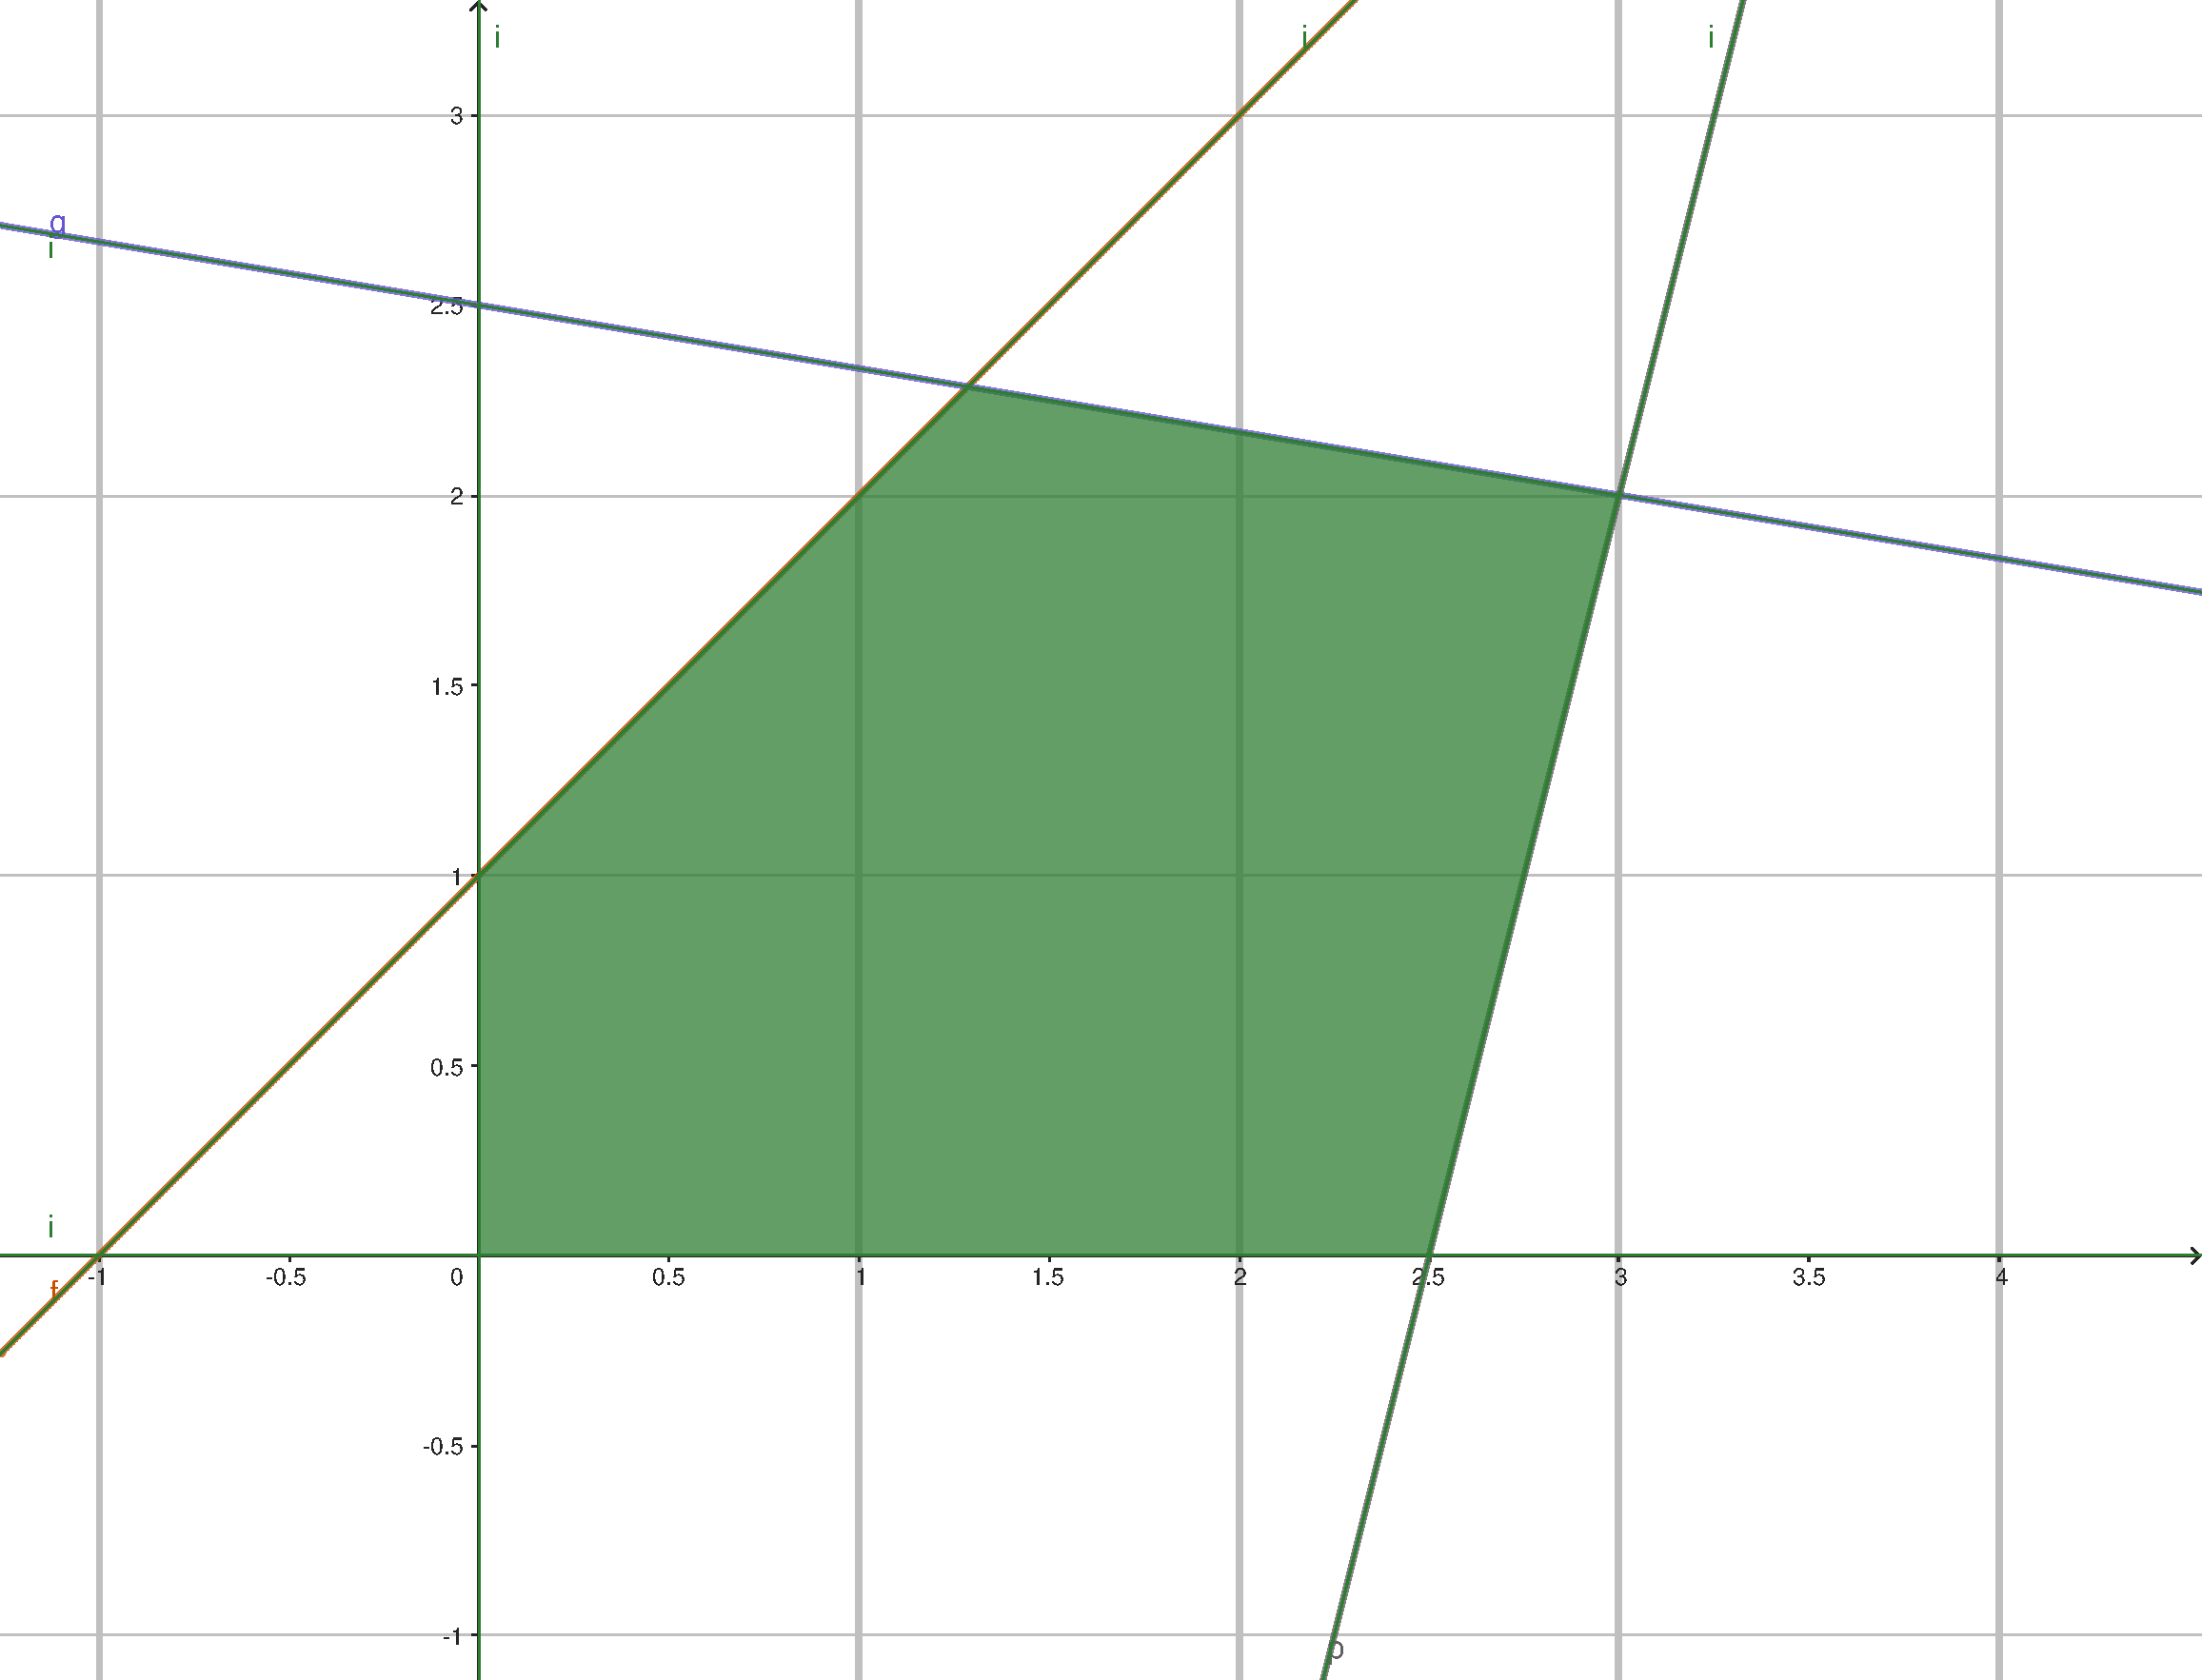
\includegraphics[width=0.4\textwidth ]{images/LP_esempio1.pdf}
        \caption{Insieme dei punti ammissibili}
        \label{LP_esempio1}
    }
\end{figure}
La funzione obiettivo essendo lineare si può rappresentare come prodotto scalare fra due vettori $\mathbf c$ e $\mathbf x$ 
$$\mathbf c^T\mathbf x=\begin{bmatrix}
    1&1
\end{bmatrix}\begin{bmatrix}
    x_1\\ x_2
\end{bmatrix} =x_1+x_2$$
Può risultare utile rappresentare sul piano anche il vettore $\mathbf c$ e la retta equivalente al sottospazio $$\text{span}(\mathbf c)=\{\alpha \mathbf c \ | \ \alpha \in \R\}$$
\begin{figure}[h]
    \centering{
        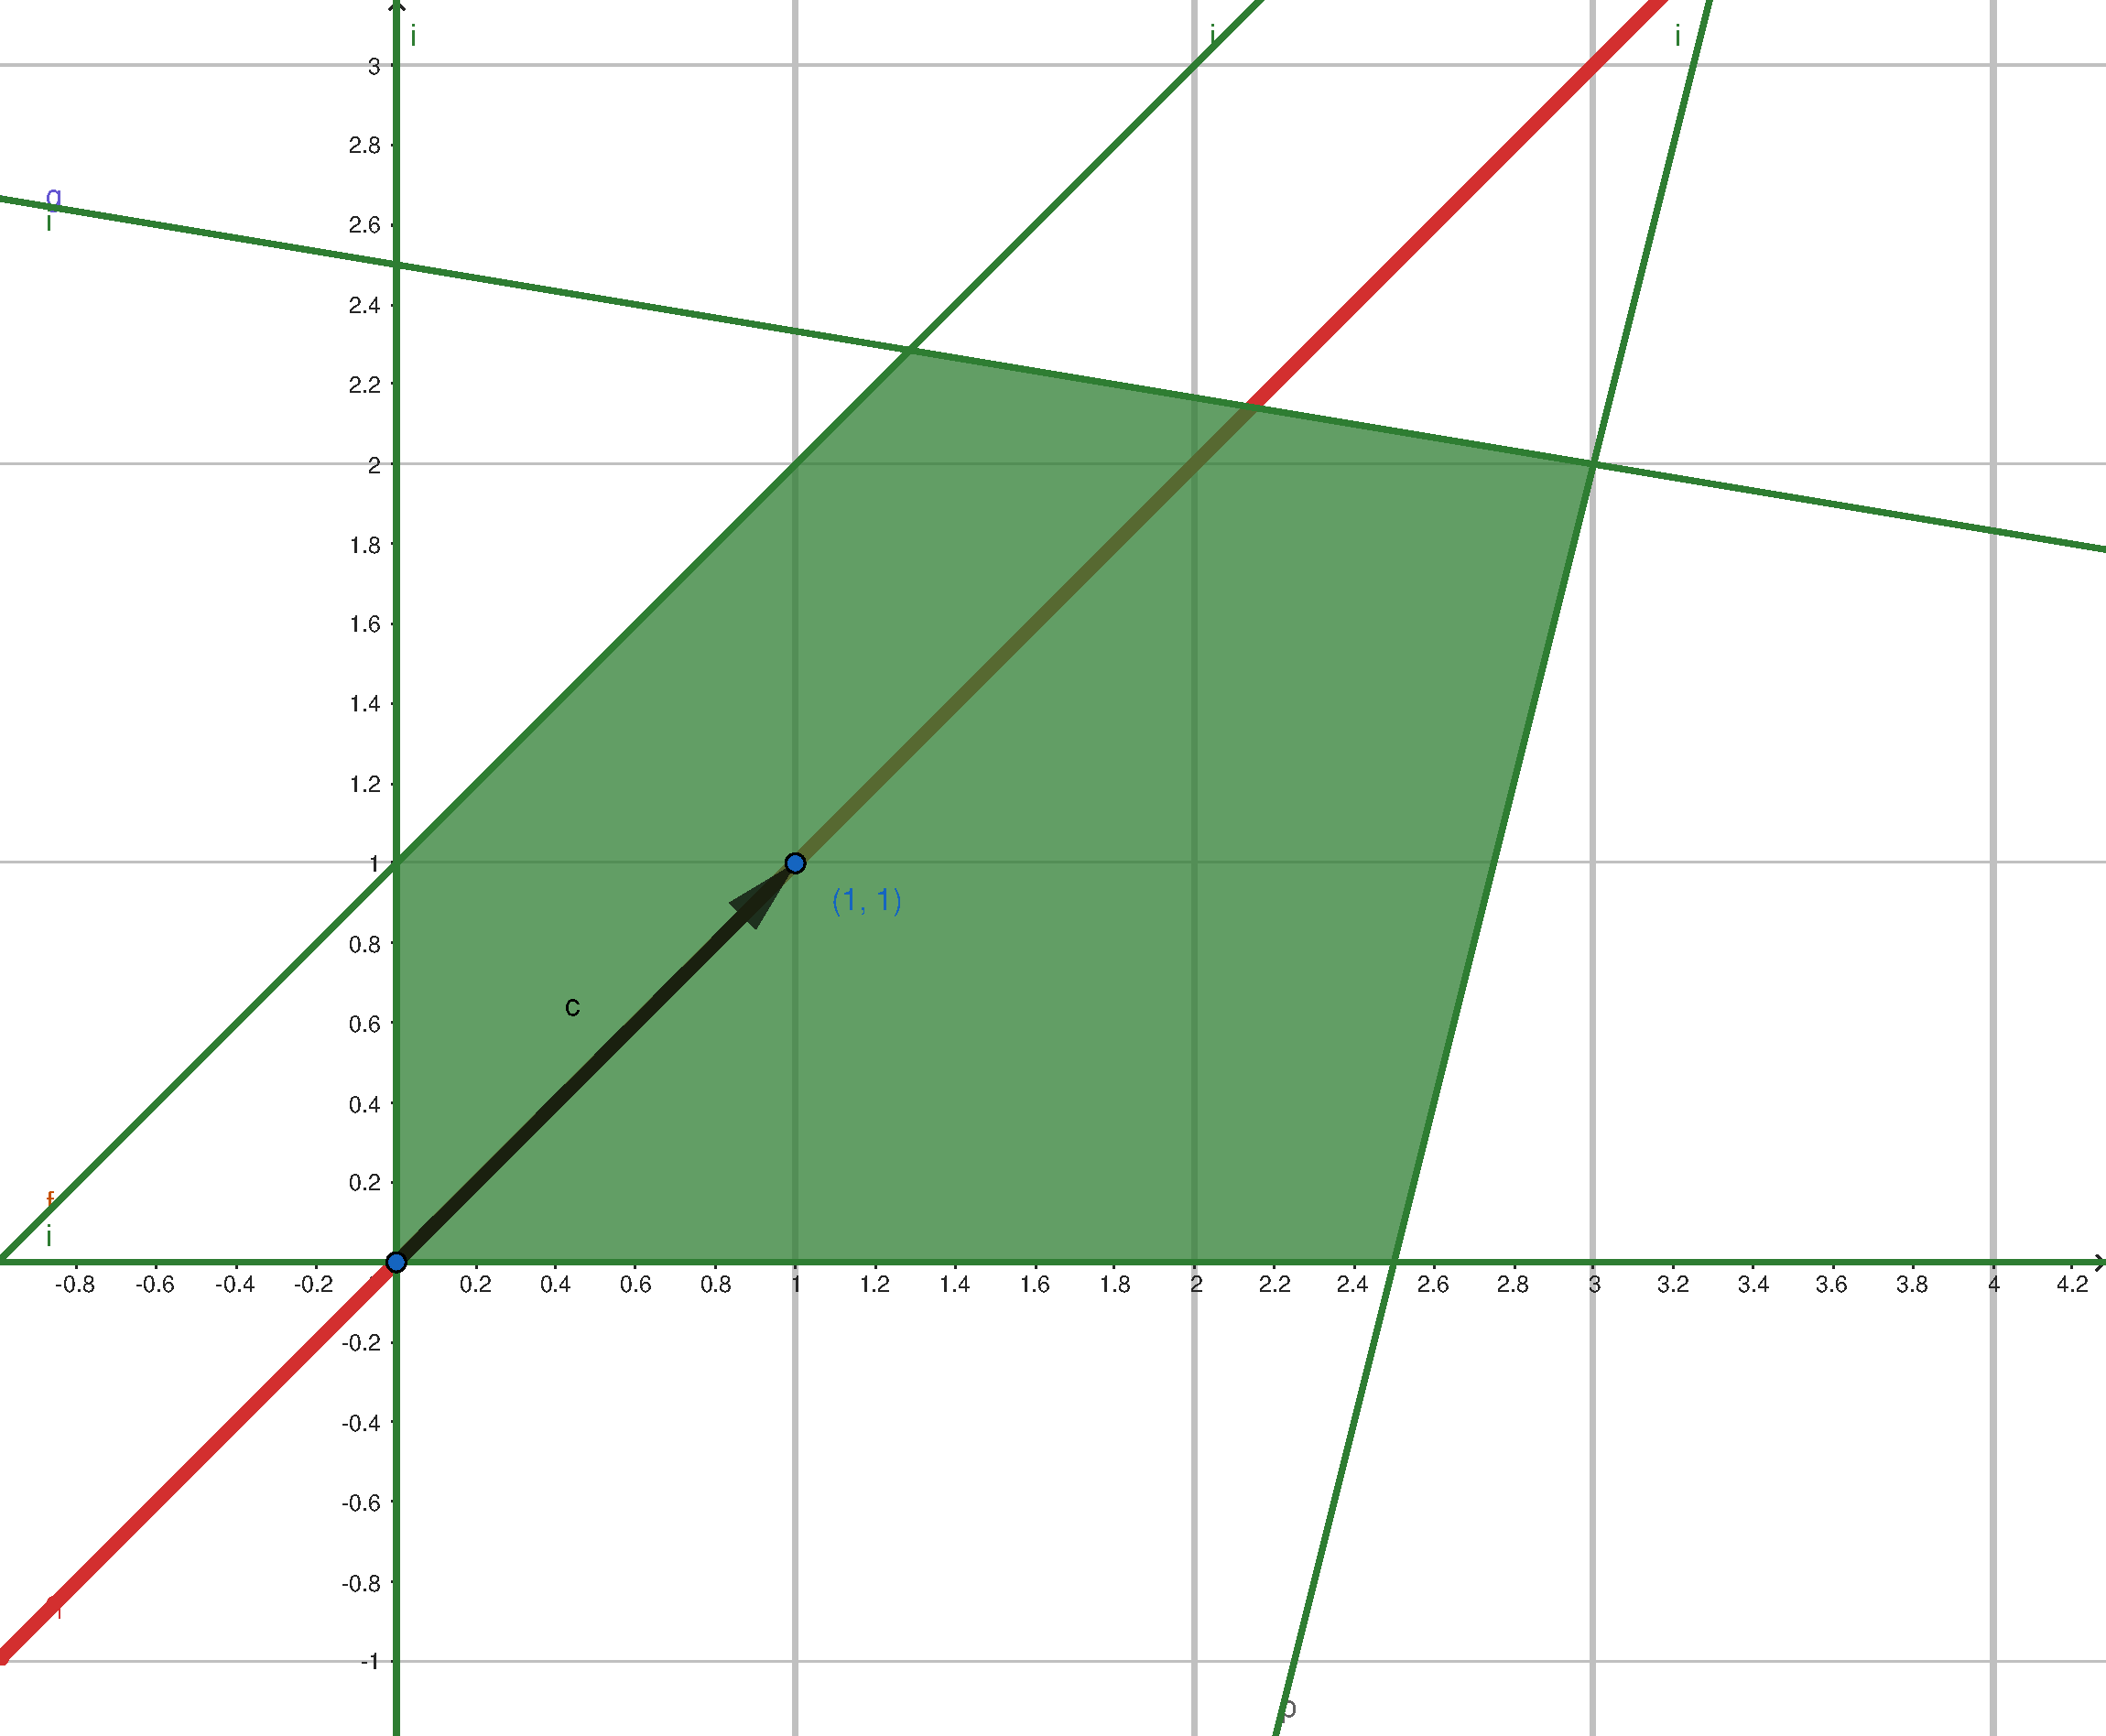
\includegraphics[width=0.4\textwidth ]{images/LP_esempio2.pdf}
    }
\end{figure}
Si consideri una retta $y'$ perpendicolare alla retta definita da $\text{span}(\mathbf c)$, i punti di $y'$ che intersecano l'insieme delle soluzioni ammissibili condividono la stessa immagine se valutati sulla funzione obiettivo. Un'interpretazione geometrica del problema può essere la seguente\begin{quotation}
    Massimizzare la funzione obiettivo equivale a trovare il massimo $\beta$ tale che l'iperpiano definito da $\mathbf c^T\mathbf x = \beta$ perpendicolare alla retta $\alpha \mathbf c$ interseca l'insieme dei punti ammissibili.
\end{quotation}
Si definisce \textbf{soluzione ottimale} ogni soluzione ammissibile che massimizza la funzione obiettivo.
\begin{figure}[h]
    \centering{
        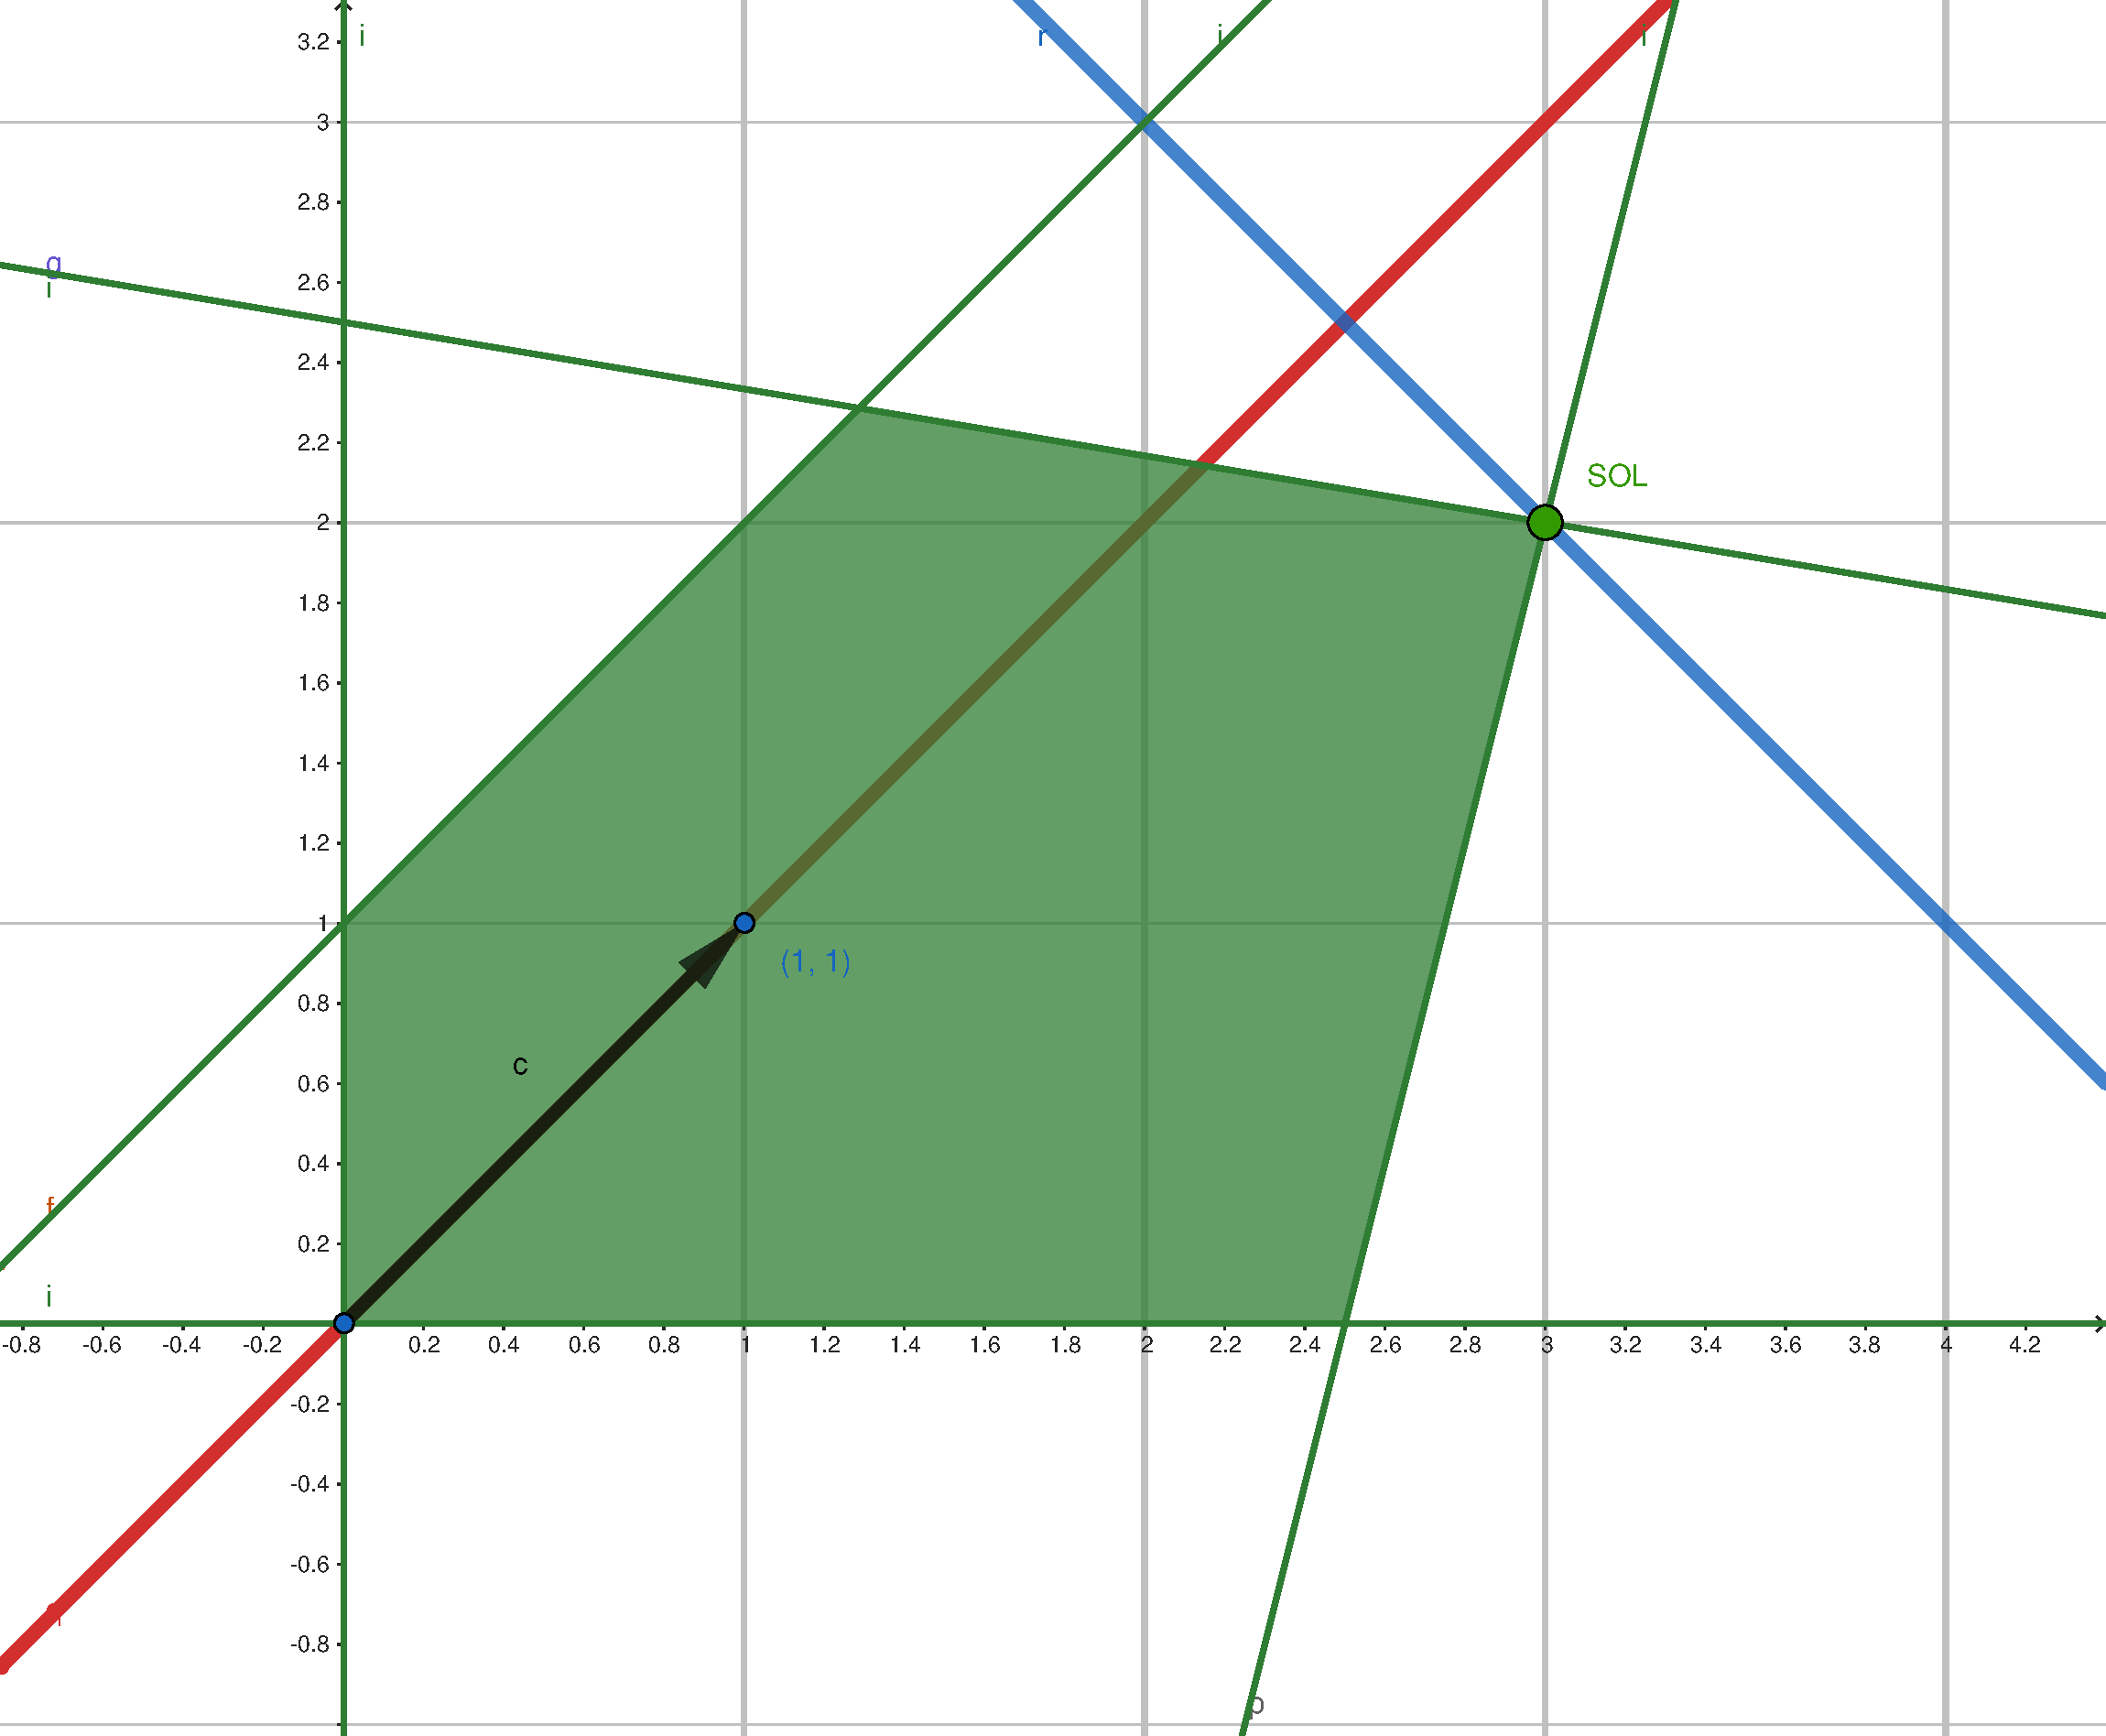
\includegraphics[width=0.4\textwidth ]{images/LP_esempio3.pdf}
    }
    \caption{Il punto $(3,2)$ è una soluzione ottimale per il programma lineare}
        \label{LP_esempio3}
\end{figure}

Il numero di soluzioni di un programma lineare può variare fra i seguenti casi\begin{enumerate}
    \item Vi è un'unica soluzione ottimale.
    \item Vi sono infinite soluzioni ottimali.
    \item Non ci sono soluzioni ammissibili, nessun punto soddisfa tutti i vincoli lineari.
    \item Non ci sono soluzioni ottimali perché il problema non è limitato, e la funzione obiettivo può essere massimizzata/minimizzata senza limiti.
\end{enumerate}
Generalmente la funzione obiettivo  $f:\R^n\rightarrow \R$ è del tipo 
$$c_1x_1+c_2x_2+\dots+c_nx_n $$
e gli $m$ vincoli sono della forma $$\begin{matrix}
    a_{11}x_1+a_{21}x_2+\dots + a_{n1}x_2\le b_1\\ 
    a_{12}x_1+a_{22}x_2+\dots + a_{n2}x_2\le b_2\\ \vdots \\ 
    a_{1m}x_1+a_{2m}x_2+\dots + a_{nm}x_2\le b_m
\end{matrix}$$
\begin{osservazione}
    Massimizzare  $\mathbf c^T \mathbf x$ equivale a minimizzare $\mathbf -\mathbf c^T\mathbf x $.
\end{osservazione}
Si può quindi assumere che un generico problema di programmazione lineare riguardi la massimizzazione di una funzione del tipo $\mathbf c^T \mathbf x$ per un fissato $\mathbf c \in \R^n$. Inoltre, ogni vincolo del tipo 
\begin{equation}\label{vincolo} a_{1i}x_1+a_{2i}x_2+\dots + a_{ni}x_n\le b_i\end{equation}
è soddisfatto dagli stessi punti che soddisfano 
$$ -a_{1i}x_1-a_{2i}x_2-\dots - a_{ni}x_2\ge b_i $$
Quindi si può assumere che ogni vincolo sia scritto nella forma \ref{vincolo}. Inoltre ogni vincolo di uguaglianza equivale a due disuguaglianze. Date le precedenti osservazioni, si può definire un'insieme di $m$ vincoli in maniera compatta tramite una matrice $m\times n $ ed un vettore $\mathbf b\in \R^m$. 
$$ A\mathbf x \le \mathbf b$$ 
Inoltre ogni vincolo di positività del tipo $x_i\ge 0$ equivale al vincolo $-x_i\le 0$. Se in un programma lineare una variabile $x_i$ può assumere qualsiasi valore in $\R$, si può sostituire con la differenza di due nuove variabili 
$$x_i=z_i-z_i' $$
ed imporre i vincoli $$ z_i,z_i'\ge 0$$ 
in tal modo è possibile, per ogni variabile del programma lineare, imporre la positività. Ciò è utile per definire una \textit{forma standard} per un programma lineare. 
\begin{definizione}\label{formaStandard}
    Un programma lineare in \textbf{forma standard} è un problema di ottimizzazione del tipo 
\end{definizione}
    $$
    \begin{matrix}
        \text{max } \ \mathbf c^T\mathbf x\\ 
        A\mathbf x \le \mathbf b\\ 
        \mathbf x \ge \mathbf  0
    \end{matrix}
    $$
Dove 
$$ 
\begin{matrix}
    \mathbf x,\mathbf c\in \R^n\\ 
    A \in \text{Mat}(m\times n)\\ 
    \mathbf b\in \R^m
\end{matrix}
$$
L'esistenza di soluzioni ammissibili dipende esclusivamente dalla matrice $A$. È impossibile che un programma lineare abbia un numero finito di soluzioni diverso da 0 e 1. In seguito verrà dimostrato che se un programma lineare ha due punti ammissibili che sono soluzione, allora ha infinite soluzioni.
\begin{definizione}
    Dati due punti $\mathbf x,\mathbf y \in \R^n$, si definisce \textbf{segmento di linea} fra i punti l'insieme \end{definizione} 
    $$ \{\alpha\mathbf x +(1-\alpha)\mathbf y \text{ t.c. }\alpha \in [0,1] \}$$
\begin{definizione}
    Un sotto-insieme $X\subseteq \R^n$ è \textbf{convesso} se la seguente è verificata 
\end{definizione}
$$\forall \mathbf x,\mathbf y \in X, \ \ \  
\{\alpha\mathbf x +(1-\alpha)\mathbf y \text{ t.c. }\alpha \in [0,1] \}\subseteq X
$$
\begin{figure}[h]
    \centering{
        \includegraphics[width=0.7\textwidth ]{images/insiemeConvesso.eps}
    }
\end{figure}
\begin{proposizione}
    L'insieme dei punti ammissibili di un programma lineare è convesso.
\end{proposizione}
\textit{Dimostrazione} : Siano $\mathbf x,\mathbf y\in \R^n$ due punti ammissibili, sia $\alpha\in[0,1]$ fissato, si considera il punto (appartenente al segmento) 
$$\alpha\mathbf x +(1-\alpha)\mathbf y $$ 
si ha che \begin{eqnarray}
    A(\alpha\mathbf x +(1-\alpha)\mathbf y)=\\ 
    \alpha A \mathbf x + (1-\alpha)A\mathbf y = \\ 
    \alpha \mathbf b + (1-\alpha )\mathbf b = \mathbf b 
\end{eqnarray}
quindi Il punto soddisfa gli $m$ vincoli
$$A(\alpha\mathbf x +(1-\alpha)\mathbf y)\le \mathbf b $$
Inoltre essendo che 
$$ \alpha \ge 0, \mathbf x \ge \mathbf  0, \mathbf y \ge 0$$
si ha che 
$$ \alpha\mathbf x +(1-\alpha)\mathbf y\ge 0$$
Quindi $\alpha\mathbf x +(1-\alpha)\mathbf y$ soddisfa tutti i vincoli del programma lineare, ed appartiene quindi ai punti ammissibili.
\hfill$\blacksquare$
\begin{proposizione}
    Se per un programma lineare esistono due soluzioni ottimali distinte $\mathbf x^*,\mathbf y^*\in \R^n$, allora tale programma lineare ha infinite soluzioni ottimali.
\end{proposizione}
\textit{Dimostrazione} : Sia $ \mathbf z$ un punto sul segmento delineato da $\mathbf x^*,\mathbf y^*$
$$\mathbf z = \alpha\mathbf x^* +(1-\alpha)\mathbf y^* \ \ \text{ per qualche }\alpha \in [0,1] $$
si ha che 
 \begin{eqnarray}
    \mathbf c^T \mathbf z = \\
    \mathbf c^T(\alpha\mathbf x^*  +(1-\alpha)\mathbf y^*)=\\
    \alpha\mathbf c^T\mathbf x^*  +(1-\alpha)\mathbf c^T\mathbf y^*
\end{eqnarray}
Essendo che $\mathbf x^*$ e $\mathbf y^*$ sono entrambe soluzioni ottimali, si ha che $c^T\mathbf x^*=c^T\mathbf y^*$
\begin{eqnarray}
    \alpha\mathbf c^T\mathbf x^*  +(1-\alpha)\mathbf c^T\mathbf y^*=\\ 
    \alpha\mathbf c^T\mathbf x^*  +(1-\alpha)\mathbf c^T\mathbf x^*=
    c^T\mathbf x^*
\end{eqnarray}
Quindi anche $\mathbf z$ è soluzione, essendo che quest'ultimo è un generico punto sul segmento, tutti i punti del segmento sono soluzioni.\hfill$\blacksquare$
\section{Applicazioni della Programmazione Lineare}
Un classico esempio di applicazione riguarda la scelta di una dieta che soddisfi dei vincoli nutrizionali minimizzando il costo degli alimenti. Vi è un'insieme di $n$ alimenti $x_1\dots,x_n$ ed ognuno di questi ha un costo $c_i$, si vuole minimizzare 
$$\sum_{i=1}^nc_ix_i $$
tenendo conto dei vincoli nutrizionali del tipo 
$$ a_{1i}x_1+a_{2i}x_2+\dots + a_{ni}x_n\ge b_i$$
Un'altro esempio riguarda la ricerca di un flusso ottimale per una network $G=(V,E,c,s,t)$, per ogni arco $(i,j)$ vi sarà una variabile $x_{ij}$ che rappresenta il flusso su tale arco, si vuole massimizzare la somma del flusso uscente dal vertice source  $s$
$$ \sum_{(s,j)\in E(G)}x_{sj}$$
I vincoli riguardano la skew simmetria, la conservazione del flusso e il vincolo delle capacità, ad esempio:
$$ \begin{matrix}
    x_{ij}\le c_{ij} \\ 
    x_{ij}=-x_{ji}
\end{matrix}$$
Un'esempio interessante di problema che si riconduce alla programmazione lineare riguarda la ricerca del cerchio di raggio massimo che può essere inscritto in un poligono.
\begin{figure}[h]
    \centering{
        \includegraphics[width=0.3\textwidth ]{images/cerchioPoligono.eps}
    }
    \caption{Cerchio inscritto nel poligono}
\end{figure}
Si assume che i lati del poligono possono essere descritti da un'insieme di rette del tipo $y=mx+b$ con $m\ne 0$.\bigskip 

Si consideri una delle rette $y=mx+b$, si vuole trovare una retta perpendicolare a questa passante per un fissato punto $(x_0,y_0)$. Questa ha equazione 
$$y=\frac{y_0-x}{m}+y_0 $$
Il punto di intersezione è $P=(x',y')$ dove 
\begin{eqnarray}
    x'=\frac{x_0+my_0}{m^2+1}-mb\\ 
    y'=m\frac{x_0+my_0-mb}{m^2+1}+b
\end{eqnarray}
\begin{figure}[h]
    \centering{
        \includegraphics[width=0.35\textwidth ]{images/rettaPassante.eps}
    }
    \caption{retta perpendicolare passante per $(x_0,y_0)$}
\end{figure}
La distanza fra $P$ e $(x_0,y_0)$, applicando la norma euclidea, risulta essere 
\begin{itemize}
    \item $\displaystyle\frac{b+mx_0-y_0}{\sqrt{1+m^2}}$ se $(x_0,y_0)$ si trova sotto la retta 
    \item $\displaystyle\frac{-b-mx_0+y_0}{\sqrt{1+m^2}}$ se $(x_0,y_0)$ si trova sopra la retta 
\end{itemize}
Il programma lineare riguarda la ricerca di un cerchio che massimizzi il raggio $r$ (distanza fra $(x_0,y_0)$ e $P$) variando fra il possibile centro $(x_0,y_0)$ all'interno del poligono, rispettando i vincoli del tipo 
\begin{itemize}
     \item$\frac{b_l+mx_0-y_0}{\sqrt{1+m^2}}\ge r, \ \ \forall  l \in {1,\dots k}$
     \item$\frac{-b_l-mx_0+y_0}{\sqrt{1+m^2}}\ge r\ \ \forall l \in {k+1,\dots n}$
\end{itemize} 
\section{Il Metodo del Simplesso}
Il metodo del simplesso è un'algoritmo per la risoluzione dei programmi lineari. Questi devono però assumere una forma differente da quella standard introdotta nella definizione \ref{formaStandard}. Un programma lineare è definito come segue 
$$
    \begin{matrix}
        \text{max } \ \mathbf c^T\mathbf x\\ 
        A\mathbf x \le \mathbf b\\ 
        \mathbf x \ge \mathbf  0
    \end{matrix}
    $$
Per ogni generica disuguaglianza del tipo 
$$ a_{1i}x_1+a_{2i}x_2+\dots + a_{ni}x_n\le b_i$$
Si considera una nuova variabile $y_i\ge 0$ detta \textbf{slack}, e la disuguaglianza diventa un'uguaglianza come segue 
$$ a_{1i}x_1+a_{2i}x_2+\dots + a_{ni}x_n+y_i = b_i$$
Vi sarà quindi un vettore $\mathbf y \in \R^m$ che viene introdotto nel problema, che assume la seguente forma 
$$
    \begin{matrix}
        \text{max } \ [\mathbf c^T \ | \ 0 \ \dots \  0]\begin{bmatrix}
            \mathbf x \\\mathbf y
        \end{bmatrix}\\ 
        [A \ | \ \text{Id}_m]\begin{bmatrix}
            \mathbf x \\ \mathbf y
        \end{bmatrix} = \mathbf b\\ 
        \begin{bmatrix}
            \mathbf x \\ \mathbf y
        \end{bmatrix} \ge 0
    \end{matrix}
    $$
Dove Id$_m$ è la matrice identità $m\times m$. Un problema LP di questo tipo è detto in \textbf{forma di equazione}, ed il metodo del simplesso opera su un programma lineare di tale forma. In generale, si scrive 
$$
    \begin{matrix}
        \text{max } \ \mathbf c^T\mathbf x\\ 
        A\mathbf x = \mathbf b\\ 
        \mathbf x \ge \mathbf  0
    \end{matrix}
    $$
\textbf{Assunzione} : Il programma lineare considerato ha almeno una soluzione ammissibile. Ossia $\exists \bar{\mathbf x}$ tale che $A\bar{\mathbf x}=\mathbf b$ e $\mathbf x \ge \mathbf  0$. Data la matrice $A$, si considerino due righe di essa, ossia $A_i$ e $A_j$, sia $A'$ un'altra matrice identica a $A$, in cui la riga $j$-esima è sostituita con la riga $A_i+A_j$
\begin{equation}
    A=\begin{bmatrix}
        a_{11}& \dots & a_{1n}\\ 
        \vdots & & \vdots \\ 
        a_{i1}& \dots & a_{in}\\ 
        \vdots & & \vdots \\ 
        a_{j1}& \dots & a_{jn}\\ 
        \vdots & & \vdots \\ 
        a_{m1}& \dots & a_{mn}
    \end{bmatrix} \ \ \ \ \ \ \  A'=\begin{bmatrix}
        a_{11}& \dots & a_{1n}\\ 
        \vdots & & \vdots \\ 
        a_{i1}& \dots & a_{in}\\ 
        \vdots & & \vdots \\ 
        a_{j1}+a_{i1}& \dots & a_{jn}+a_{in}\\ 
        \vdots & & \vdots \\ 
        a_{m1}& \dots & a_{mn}
    \end{bmatrix}
\end{equation}
Se $\mathbf x$ soddisfa $A\mathbf x = \mathbf b$ allora soddisfa anche $A'\mathbf x = \mathbf b'$ dove $\mathbf b'$ è identico a $\mathbf b$ ma il $j$-esimo elemento è sommato all'$i$-esimo $$ \mathbf b' = [b_1 \ \ \dots b_i \ \ \dots \ \ b_i+b_j \ \ \dots b_n]^T$$
Le operazioni sulle righe di $A$ non cambiano l'insieme delle soluzioni, si assume che le righe siano \textit{linearmente indipendenti}, che il rango di $A$ sia $m$, e che lo span delle righe di $A$ è un sottospazio di $\mathbb{R}^n$.\begin{proposizione}
    Il rango delle colonne di $A$ è $m$, la dimensione del sottospazio di $\mathbb R^m$ dato dallo span delle colonne è $m$.
\end{proposizione}
La dimostrazione è omessa.\bigskip

\noindent
Il problema descritto è \begin{eqnarray}
    A\mathbf x = \mathbf b \\ \mathbf x \ge \mathbf  0 \\ \text{esiste una soluzione}\\ 
    \text{rango righe di }A=\text{rango colonne di }A=m
\end{eqnarray}
Considerando $\ker(A)=\{\mathbf x \text{ t.c. }A\mathbf x = \mathbf 0\}$ si ha un sottospazio di dimensione $n-m$ di $\mathbb R^n$, lo spazio delle soluzioni di $A\mathbf x = \mathbf b$ è un \textbf{sottospazio affine} e si ottiene sommando $\mathbf b$ a tutti i vettori di $\ker(A)$.\bigskip 
\subsection{Soluzioni Ammissibili Basiche}
\textit{Esempio} : Si consideri il triangolo delineato dai punti $(0,0,3),(0,3,0),(3,0,0)$, tutti i punti di tale triangolo sono i vettori $\mathbf x\ge \mathbf 0$ che soddisfano $A\mathbf x = \mathbf b$.\begin{figure}[h]
    \centering{
        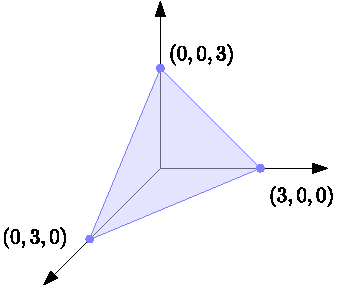
\includegraphics[width=0.35\textwidth ]{images/triangolo.pdf}
    }
    \caption{triangolo in $\mathbb R^3$}
\end{figure}
Si ha $A=[1 \ \ 1 \ \ 1]$ e $b=3$
$$ \begin{bmatrix}
    1 & 1 & 1
\end{bmatrix}\begin{bmatrix}
    x \\ y \\ z
\end{bmatrix}=3\implies x+y+z=3$$
I 3 vertici del triangolo rappresentano delle soluzioni "speciali", ottenute ponendo 2 delle 3 variabili uguali a zero e risolvendo per le altre, tali soluzioni sono dette \textit{basiche}.\bigskip 

In generale, $A\in Mat(m\times n)$ e $\mathbf b \in \mathbb R^n$, si vogliono porre un numero massimale di variabili pari a zero e risolvere per le altre, si pongono esattamente $n-m$ variabili nulle. 

Sia $\mathcal B \subseteq \{1,\dots n\}$ l'insieme degli indici $i$ per cui la variabile $x_i$ non è posta a zero, e sia $A_{\mathcal B}$ la sotto-matrice di $A$ composta dalle colonne il cui indice è relativo ad una variabile diversa da zero.
$$ \begin{bmatrix}
    a_{1i} & \dots & a_{mi}
\end{bmatrix}^T \text{ è una colonna di }A_{\mathcal B} \iff i\in\mathcal B$$
Sia $\mathbf b_{\mathcal B}$ definito in maniera intuitiva, come il vettore contenente la componente $j$-esima di $\mathbf b$ se $j\in \mathcal B$. Si considera il problema derivato \begin{equation}
    A_{\mathcal B}\mathbf x_{\mathcal B}=\mathbf b_{\mathcal B} \ \ \ \ A_{\mathcal{B}}\in Mat(m\times m)
\end{equation}
Se $A_{\mathcal{B}}$ non è \textbf{singolare} (il determinante è diverso da zero) allora esiste una soluzione $\bar{ \mathbf x}$ per il problema derivato, se $\bar{ \mathbf x}\ge 0$, allora è anche una soluzione per il problema originale, ponendo a zero tutte le componenti della soluzione i cui indici non sono in $\mathcal B$.\begin{itemize}
    \item se $\bar{ \mathbf x}=[x_{k1} \ \ x_{k2} \ \ \dots \ \ x_{km}]^T$ è soluzione di  $ A_{\mathcal B}\mathbf x_{\mathcal B}=\mathbf b_{\mathcal B}$
    \item si ha $\{k1,k2\dots, km\}=\mathcal B$
    \item allora il vettore $\bar{ \mathbf x}'$ con\begin{itemize}
        \item $x_i = x_{kj}$ se $i=kj$ per qualche $j\le m$, ossia $i\in\mathcal B$
        \item $x_i = 0 $ se $i \notin \mathcal B$
    \end{itemize}
    è soluzione di $A\mathbf x = \mathbf b$ se $\bar{ \mathbf x}'\ge 0$.
\end{itemize}
\begin{definizione}
    Dato un programma lineare $$
    \begin{matrix}
        \text{max } \ \mathbf c^T\mathbf x\\ 
        A\mathbf x \le \mathbf b\\ 
        \mathbf x \ge \mathbf  0
    \end{matrix}
    $$
    Una soluzione ammissibile $\bar{\mathbf x}$ è detta \textbf{basica} (BFS) se esiste un sotto-insieme di indici $\mathcal B\subseteq \{1,2,\dots n\}$ tale per cui\begin{itemize}
        \item $A_{\mathcal B}$ non è singolare 
        \item $\bar{x}_j=0$ $\forall j \notin \mathcal{B}$
    \end{itemize}
\end{definizione}
\textit{Esempio} : Data la matrice \begin{equation}
    A=\begin{bmatrix}
        1&6&3&-3&4\\ 
        0&1&3&2&4
    \end{bmatrix}
\end{equation}
Ed il sistema di equazioni 
$$ A\mathbf x = \begin{bmatrix}
    6\\6
\end{bmatrix}$$
Per la base  $\mathcal B = \{2,4\}$ si ha $$A_{\mathcal B}=\begin{bmatrix}
    6&-3\\1&2
\end{bmatrix} $$
La matrice non è singolare, per il sistema $$ \begin{bmatrix}
    6&-3\\1&2
\end{bmatrix}\begin{bmatrix}
    x_2\\x_4
\end{bmatrix}  = \begin{bmatrix}
    6\\6
\end{bmatrix}$$
una soluzione è $$ \begin{bmatrix}
    2\\2
\end{bmatrix}$$
Quindi una soluzione ammissibile basica per il problema originale è 
$$ \bar{\mathbf x}=\begin{bmatrix}
    0&2&0&2&0
\end{bmatrix}^T$$
Se considerassimo la base $\mathcal B' = \{3,5\}$, si avrebbe la sotto-matrice 
$$A_{\mathcal B'}= \begin{bmatrix}
    3&4\\3&4
\end{bmatrix}$$
Essendo singolare, per tale base non esiste alcuna soluzione basica.
\begin{proposizione}\label{insiemeK}
    Sia $A\mathbf x=b$, $\mathbf x \ge  \mathbf 0$ un programma lineare, e sia $\mathbf{\bar x}$ una BFS (soluzione ammissibile basica), si consideri l'insieme di indici 
    $$ K=\{i \text{ t.c. }\bar x_i>0\}$$
    Le colonne della matrice $A_K$ sono linearmente indipendenti. 
\end{proposizione}
\textit{Dimostrazione} : La dimostrazione è banale, esiste una base $\mathcal B$ a cui $\mathbf{\bar x}$ fa riferimento per cui $K\subseteq \mathcal B$, essendo le colonne di $A_{\mathcal B}$ linearmente indipendenti, anche un loro sotto-insieme, ossia quelle di $A_K$ lo sono.\hfill$\blacksquare$
\begin{proposizione}
    Si consideri un programma lineare, sia $\mathbf{\bar x}$ una soluzione ammissibile e $$ K=\{i \text{ t.c. }\bar x_i>0\}$$ $\mathbf{\bar x}$ è una BFS se e solo se le colonne di $A_K$ sono linearmente indipendenti.
\end{proposizione}
\textit{Dimostrazione} : Verrà dimostrata solo una delle due implicazioni, si assume che $\mathbf{\bar x}$ è una soluzione ammissibile e che le colonne di $A_K$ siano linearmente indipendenti. Per dimostrare che $\mathbf{\bar x}$ sia una BFS è necessario trovare una base che contenga $K$.

Sia $\mathcal B^*$ un'insieme definito come segue\begin{enumerate}
    \item $K\subseteq\mathcal B^*$
    \item Le colonne di $\mathcal B^*$ sono linearmente indipendenti 
    \item $\mathcal B^*$ è l'insieme massimale che rispetti le due condizioni precedenti
\end{enumerate}
Bisogna mostrare che $\mathcal B^*$ ha $m$ elementi in modo tale che $A_{\mathcal B^*}$ sia una matrice quadrata $m\times m$.

Si assuma che $|\mathcal B^*|<m$, ciò significherebbe che le restanti colonne di $A$ sono contenute nello span delle colonne di $A_{\mathcal B^*}$, quindi $A$ ha \textit{meno} di $m$ colonne linearmente indipendenti, ma è noto che il rango di $A$ sia $m$, quindi l'assunzione  $|\mathcal B^*|<m$ porta ad una contraddizione $\implies |\mathcal B^*|=m$.\hfill$\blacksquare$
\begin{osservazione}
    Ogni base ha almeno una BFS associata.
\end{osservazione}
\textbf{Conclusione} : Esiste un numero finito di BFS. Ogni base è un sotto-insieme di $m$ elementi preso da $\{1,2,\dots n\}$, quindi esistono al più $\binom{n}{m}$ basi distinte, quindi esistono al più $\binom{n}{m}$  BFS.\bigskip 

Il seguente risultato è fondamentale in quanto stabilisce che un programma lineare (che riguarda la ricerca di una soluzione fra un'insieme non numerabile) si può ridurre ad un problema di ottimizzazione combinatoria.
\begin{teorema}\label{teo:BFS}
    Si consideri un programma lineare in forma di equazione
$$ 
\begin{matrix}
    \text{max } \ \mathbf c^T\mathbf x\\ 
    A\mathbf x = \mathbf b\\ 
    \mathbf x \ge  \mathbf 0
\end{matrix}
$$\begin{enumerate}
    \item Se esiste almeno una soluzione ammissibile ed il problema è limitato (l'insieme delle soluzioni ammissibili è compatto), allora esiste una soluzione ottimale.
    \item Se esiste una soluzione ottimale, allora esiste anche una BFS che è a sua volta ottimale.
\end{enumerate}
\end{teorema}
La dimostrazione del teorema \ref{teo:BFS} richiede alcuni passi preliminari. \acc 
\textbf{Statement} $\star$ : Se la funzione obiettivo di un LP in forma di equazione è limitata superiormente, allora per ogni soluzione ammissibile $\mathbf y$ esiste una BFS $\mathbf z$ tale che $\mathbf c^T\mathbf z\ge \mathbf c^T\mathbf y$.\acc 
\textbf{Claim 1} : Se $\star$ è vera, allora il teorema è dimostrato.\acc 
\textit{Dimostrazione Claim 1} : Si consideri la BFS $\mathbf y$ che massimizza la funzione obiettivo rispetto tutte le altre BFS. Assumiamo che $\mathbf y$ non sia ottimale, allora esiste $\mathbf y^*$ (che non è una BFS) tale che 
$$\mathbf c^T\mathbf y^*\ge \mathbf c^T\mathbf y$$
Ma per il claim $\star$ esiste una BFS $\mathbf z$ tale per cui 
$$\mathbf c^T\mathbf z\ge\mathbf c^T\mathbf y^*\ge \mathbf c^T\mathbf y$$
Ciò va in contraddizione con l'assunzione che $\mathbf y$ sia massimale fra le BFS, quindi non può esistere tale $\mathbf y^*\implies \mathbf y$ è una BFS ottimale $\implies$ il claim è dimostrato : $\star \implies $ teorema \ref{teo:BFS}.\hfill$\blacksquare$\bigskip

Per dimostrare il teorema è quindi sufficiente dimostrare lo Statement $\star$.
Sia $\mathbf y$ un'arbitraria soluzione ammissibile, sia $\mathbf z$ un'altra soluzione ammissibile tale che \begin{enumerate}
    \item $\mathbf  c^T\mathbf z\ge \mathbf  c^T\mathbf y$
    \item $\mathbf z$ ha un numero massimale di componenti uguali a zero
\end{enumerate}
Tale $\mathbf z$ esiste dato che nel caso peggiore si può considerare $\mathbf z = \mathbf y$. Si consideri l'insieme $K$ degli indici delle componenti positive di $\mathbf z$ 
$$ K=\{j \text{ t.c. }z_j>0\}$$
La proposizione \ref{insiemeK} afferma che se le colonne di $A_K$ sono linearmente indipendenti $\mathbf z$ è una BFS, ciò dimostrerebbe lo Statement $\star$.

Si assuma  che le colonne di $A_K$ siano linearmente dipendenti. Sia $k=|K|$. Esistono dei coefficienti $\alpha_1\dots, \alpha_k$ tali per cui 
\begin{equation}\label{linDIP}
    \alpha_1\begin{bmatrix}
        \\A^1_K\\ \\
    \end{bmatrix}+\dots + \alpha_k\begin{bmatrix}
        \\A^k_K\\ \\
    \end{bmatrix}=\mathbf 0\implies 
\end{equation}\begin{equation}\label{linDIP2}
    A_K\begin{bmatrix}
        \alpha_1\\\vdots\\\alpha_k 
    \end{bmatrix}=\mathbf 0
\end{equation}
Si consideri un particolare vettore $\mathbf w$ definito come segue\begin{itemize}
    \item la componente $j$-esima di $\mathbf w$ contiene $\alpha_j$ se $j\in K $, $\alpha_j$ è il coefficiente moltiplicato alla colonna $j$-esima di $A_K$ nella combinazione lineare dell'equazione  \ref{linDIP}.
    \item Se $j\notin K$, allora la componente $j$-esima di $\mathbf w$ è 0.
\end{itemize}
Data l'equazione \ref{linDIP2}, risulta chiaro che il prodotto della matrice originale $A$ e $\mathbf w$ sia uguale al prodotto fra $A_K$ ed il vettore dei coefficienti $\alpha_1\dots,\alpha_k$. 
\begin{equation}\label{linDIP3}
   A\mathbf w= A_K\begin{bmatrix}
        \alpha_1\\\vdots\\\alpha_k 
    \end{bmatrix}=\mathbf 0
\end{equation}
Riconsiderando la soluzione $\mathbf z$, si può sommare a $\mathbf w$ e moltiplicare per la matrice $A$ 
$$ A(\mathbf z+\mathbf w)=A\mathbf z+A\mathbf w=A\mathbf z+\mathbf 0 = \mathbf b+\mathbf 0 = \mathbf b$$
Essendo che $\mathbf z$ è soluzione il prodotto fra quest'ultimo ed $A$ è uguale al vettore $\mathbf b$ relativo ai vincoli del programma lineare. Nonostante $\mathbf z+\mathbf w$ soddisfi i vincoli, non è certo che sia soluzione, in quanto non è certo se abbia o no componenti negative (si ricordi che una soluzione deve essere maggiore o uguale al vettore $\mathbf 0$).

Si noti come per definizione di $\mathbf w$, questo ha una componente uguale a zero in una data posizione, se in quella data posizione la soluzione $\mathbf z$ ha la componente uguale a zero, quindi $\mathbf w$ ha \textit{almeno tanti} zeri quanti quelli di $\mathbf z$.\acc 
\textbf{Claim 2} : Il vettore $\mathbf w$ soddisfa le seguenti\begin{enumerate}
    \item $\mathbf c^T\mathbf w \ge 0$
    \item $\exists j\in K \text{ t.c. }w_j<0$
\end{enumerate}
\textit{Dimostrazione} : Se per $\mathbf w$ il punto (2) non dovesse essere soddisfatto, si potrebbe considerare $-\mathbf w$, questo soddisfa tutte le condizioni per cui è stato definito $\mathbf w$ : $A(-\mathbf w)=A\mathbf w =\mathbf 0$. Tale sostituzione si può considerare anche per soddisfare il punto (1), nel caso in cui si dovesse verificare che $c^T\mathbf w<0$.

Se la condizione (2) non dovesse essere soddisfatta, allora si consideri il vettore (in funzione di $t\in\mathbb R^+$)  $$\mathbf z(t)=\mathbf{z}+t\mathbf w$$
Tale vettore soddisfa i vincoli del programma lineare 
$$A\mathbf z(t)=A(\mathbf z + t\mathbf w)=A\mathbf z+tA\mathbf w=\mathbf b + t\cdot \mathbf 0 = \mathbf b $$
Inoltre essendo la (2) non soddisfatta, si ha che, per ogni possibile $t\in\mathbb R^+$ $$ z(t)_j=z_j+tw_j\ge 0$$ questo perché \begin{enumerate}
    \item $z_j\ge 0$ essendo $\mathbf z$ una soluzione 
    \item $t$ è non negativo perché varia in $\mathbb  R^+$
    \item $w_j$ non è negativo dato che la (2) non è soddisfatta
\end{enumerate}
Essendo $\mathbf z(t)$ sempre maggiore o uguale a zero si ha: \begin{equation}
    \mathbf c^T \cdot \mathbf z(t)= \mathbf c^T (\mathbf z + t\mathbf w)=\mathbf c^T \mathbf z + t\mathbf c^T \mathbf w
\end{equation}
Attenzione, essendo il punto (1) soddisfatto, $c^T \mathbf w$ è positivo, quindi dato il termine $t\mathbf c^T \mathbf w$, la funzione $ \mathbf c^T \cdot \mathbf z(t)$ non è limitata, ciò è una contraddizione, quindi le due assunzioni del claim sono vere. \hfill$\blacksquare$\bigskip

Dato ciò, esiste un indice $j\in K$ per cui $w_j<0$, si consideri nuovamente il vettore $$\mathbf z(t)=\mathbf{z}+t\mathbf w$$
Avendo verificato che questo soddisfa i vincoli $\forall t$, ci si pone la domanda, che valore assume nella funzione obiettivo? 
$$ \mathbf c^T \mathbf z(t)=\mathbf c^T\mathbf z+t\mathbf c^T\mathbf w$$
Sappiamo che\begin{itemize}
    \item $\mathbf c^T\mathbf z\ge \mathbf c^T\mathbf y$ per la scelta di $\mathbf z$
    \item $t\mathbf c^T\mathbf w\ge 0$ per il claim
\end{itemize}
Ne consegue che $$ \mathbf c^T \mathbf z(t)\ge \mathbf c^T \mathbf y$$
Per la chiarezza della dimostrazione, si ricordi che $\mathbf z$ è stato scelto per soddisfare le seguenti \begin{enumerate}
    \item $\mathbf  c^T\mathbf z\ge \mathbf  c^T\mathbf y$
    \item $\mathbf z$ ha un numero massimale di componenti uguali a zero
\end{enumerate}
$$ 
\mathbf z(t)=\begin{bmatrix}
    0\\\vdots \\ z_i\\ \vdots \\0
\end{bmatrix}+t\begin{bmatrix}
    0\\\vdots \\ w_i\\ \vdots \\0
\end{bmatrix}
$$
sia $ w_i$ una componente negativa di $\mathbf w$, se $t=-\frac{z_i}{w_i}$ allora 
$$ 
\mathbf z(-\frac{z_i}{w_i})=\begin{bmatrix}
    0\\\vdots \\ z_i\\ \vdots \\0
\end{bmatrix}-\frac{z_i}{w_i}\begin{bmatrix}
    0\\\vdots \\ w_i\\ \vdots \\0
\end{bmatrix}\implies z(-\frac{z_i}{w_i})_i=z_i-z_i=0
$$
Il vettore $\mathbf z(-\frac{z_i}{w_i})$ ha una componente  nulla in più rispetto a $\mathbf z$, se si considera $$ t^*=\min_{i \text{ t.c. }w_i<0}(-\frac{z_i}{w_i})$$
il vettore $\mathbf z(t^*)$ risulterà non negativo, quindi: 
$$\begin{matrix}
    A\mathbf z(t^*=\mathbf b)\\ \mathbf z(t^*)\ge 0
\end{matrix}$$
Il vettore $\mathbf z(t^*)$ è una soluzione ammissibile ed ha uno 0 in più rispetto a $\mathbf z$, ma questa è una contraddizione (data la scelta di $\mathbf z$), quindi è impossibile che le colonne di $A_K$ siano linearmente dipendenti $\implies$ $\mathbf z$ è una BFS, lo Statement $\star$ è dimostrato.\hfill$\blacksquare$\acc 
\textbf{Corollario} : Se un programma lineare ha una funzione obiettivo limitata, allora esiste un'algoritmo che trova una soluzione ottimale in un numero finito di passi.
\subsection{Ricerca sul Poliedro}\label{RicercasulPoliedro} 
Si consideri il seguente programma lineare$$\begin{matrix}
    \max \ x_1+x_2\\ -x_1+x_2\le 1 \\ x_1\le 3 \\ x_2 \le 2 \\ x_1,x_2 \ge 0
\end{matrix}$$
L'insieme delle soluzioni ammissibili è mostrato in figura \ref{fig:solEsempio}.
\begin{figure}[h]\label{fig:solEsempio}
    \centering{
        \includegraphics[width=0.35\textwidth ]{images/insiemeSoluzioniLP1.eps}
    }
    \caption{Insieme definito dai vincoli}
\end{figure}
Per trasformare il problema in forma di equazione occorre aggiungere 3 variabili slack $x_3,x_4,x_5$.$$\begin{matrix}
    \max \mathbf{c}^T \mathbf x  \ \\ -x_1+x_2+x_3= 1 \\ x_1+x_4= 3 \\ x_2 +x_5= 2 \\ x_1,x_2,x_3,x_4,x_5 \ge 0
\end{matrix}$$
in forma matriciale:
$$A=\begin{bmatrix}
    -1&1&1&0&0\\ 
    1&0&0&1&0 \\ 
    0& 1 & 0 & 0 & 1
\end{bmatrix}  \ \ \ \ \mathbf c = \begin{bmatrix}
    1 & 1 & 0&0&0
\end{bmatrix}^T$$
Si consideri la base $\mathcal B = \{1,2,4\}$ : 
$$A_{\mathcal B}=\begin{bmatrix}
    -1&1&0\\ 1&0&1\\0&1&0
\end{bmatrix} 
$$
è non singolare, si può risolvere il sistema di equazioni 
\begin{eqnarray}\begin{bmatrix}
    -1&1&0\\ 1&0&1\\0&1&0
\end{bmatrix} \begin{bmatrix}
    x_1\\x_2\\x_4
\end{bmatrix}=\begin{bmatrix}
    1\\ 3\\ 2
\end{bmatrix}\implies  \begin{cases}
    x_1=1\\x_2=2\\x_4=2
\end{cases}
\end{eqnarray}
La BFS è $\mathbf x = \begin{bmatrix}
    1&2&0&2&0
\end{bmatrix}^T$
Le variabili slack $x_3,x_5$ della soluzione $\mathbf x$ sono poste a zero, ciò significa che tale punto soddisfa i vincoli del problema originale (in forma di uguaglianza), in particolare, soddisfa le eguaglianze del primo e del terzo vincolo $$ \begin{matrix}
    -x_1+x_2= 1 \\ x_2 = 2
\end{matrix}$$ 
Tale punto può essere geometricamente individuato nell'insieme delle soluzioni ammissibili del problema originale, ed equivale al punto su cui si intersecano le due rette che definiscono il primo ed il terzo vincolo, come mostrato in figura \ref{fig:solEsempio2}.
\begin{figure}[h]\label{fig:solEsempio2}
    \centering{
        \includegraphics[width=0.35\textwidth ]{images/insiemeSoluzioniLP2.eps}
    }
    \caption{punto di intersezione}
\end{figure}
\begin{definizione}
    Un'insieme $\mathcal X\subset \mathbb R^n$ è \textbf{aperto} se $\forall \mathbf x\in \mathcal X$, $\exists \epsilon >0$ tale che $\{\mathbf y\in \mathbb R^n \ | \ \|\mathbf y-\mathbf x\|\le \epsilon   \}\subset \mathcal X$.
\end{definizione}
\begin{definizione}
    Un'insieme $\mathcal X\subset \mathbb R^n$ è \textbf{chiuso} se il suo complemento $\mathbb R^n \backslash \mathcal X$ è un'insieme aperto.
\end{definizione}
\begin{osservazione}
    L'unione di due insiemi aperti è un'insieme aperto. L'intersezione di due insiemi chiusi è un'insieme chiuso.
\end{osservazione}
\begin{definizione}
    Dato un sotto-insieme di punti  $I\subset \mathbb R^n$, si definisce il suo \textbf{inviluppo convesso} l'intersezione di tutti i sotto-insiemi convessi di $\mathbb R^n$ contenenti $I$. Alternativamente, si può dire che l'inviluppo convesso di $I$ è il più piccolo insieme convesso contenente $I$.
\end{definizione}
\begin{figure}[h]
    \centering{
        \includegraphics[width=0.4\textwidth ]{images/inviluppoConvesso.eps}
    }
    \caption{inviluppo convesso dei punti $x_1,x_2\dots,x_5$}
\end{figure}
\begin{definizione}
    Dati $n$ punti $\mathbf{x}_1,\mathbf{x}_2\dots ,\mathbf{x}_n\subset \mathbb R^m$, una loro \textbf{combinazione convessa} è un punto $\mathbf{z}$ definito come segue \begin{itemize}
        \item $\displaystyle\mathbf z =  \sum_{i=1}^n\alpha_i\mathbf x_i$
        \item $\alpha_i\ge 0  \ \ \ \forall i$
        \item $\displaystyle  \sum_{i=1}^n\alpha_i=1$
    \end{itemize}
\end{definizione}
\begin{osservazione}
    Una combinazione convessa fra due punti è un segmento di linea.
\end{osservazione}
\begin{proposizione}
    Siano  $\mathbf{x}_1,\mathbf{x}_2\dots ,\mathbf{x}_n$ dei punti in $\mathbb R^m$, sia $C$ l'inviluppo convesso di tali punti, e sia $\tilde C$ l'insieme di tutte le combinazioni convesse $$\tilde{C} =
     \Big\{\sum_{i=1}^n \alpha_i\mathbf{x}_i \text{ t.c. }\alpha_i\ge 0 \ \forall i,\ \sum_{i=1}^n \alpha_i=1\Big\} $$
    si ha che $C=\tilde C$
\end{proposizione}
\textit{Dimostrazione} : La dimostrazione procederà classicamente con una doppia inclusione. Si vuole mostrare come prima cosa che $C\subseteq \tilde C$, essendo $C$ l'intersezione di tutti gli insiemi convessi contenenti i punti, ed essendo che $\tilde C$ contiene ogni punto $\mathbf x_i$, è sufficiente mostrare che $\tilde C$ sia convesso.

Siano $\mathbf z_1,\mathbf z_2\in\tilde C$, ossia della forma\begin{eqnarray*}
    \mathbf z_1 = \sum_i\alpha_i\mathbf x_i, \ \ \ \  \alpha_i\ge 0, \ \sum_1\alpha_i=1\\ 
    \mathbf z_2 = \sum_i\beta_i\mathbf x_i, \ \ \ \  \beta_i\ge 0, \ \sum_1\beta_i=1
\end{eqnarray*}
Un generico punto sul segmento di $\mathbf z_1,\mathbf z_2$ è 
$$ t\mathbf z_1+(1-t)\mathbf z_2, \ \ \ \ t\in[0,1]$$
esplicitando\begin{eqnarray}
    t\displaystyle  \sum_i\alpha_i\mathbf x_i+(1-t)\mathbf \displaystyle  \sum_i \beta_i\mathbf x_i=\\ \displaystyle  
    \displaystyle  \sum_i t\alpha_i\mathbf x_i+\mathbf \displaystyle  \sum_i (1-t)\beta_i\mathbf x_i=\\ \displaystyle  
    \sum_i(t\alpha_i+(1-t)\beta_i)\mathbf x_i
\end{eqnarray}
Bisogna mostrare che $\sum_i(t\alpha_i+(1-t)\beta_i)\mathbf x_i$ è una combinazione convessa, essendo che $$ t\ge 0, \ \alpha_i\ge 0, \ \beta_i\ge 0$$
è immediato che, per ogni $i$ si ha che $t\alpha_i+(1-t)\beta_i\ge 0$, inoltre \begin{eqnarray}
    \sum_i t\alpha_i+(1-t)\beta_i=\\ 
    \sum_it\alpha_i+\sum_i(1-t)\beta_i=\\ 
    t\sum_i\alpha_i+(1-t)\sum_i\beta_i
\end{eqnarray}
Essendo che per ipotesi $\sum_i\alpha_i=\sum_i\beta_i=1$, si ha che \begin{eqnarray}
    t\sum_i\alpha_i+(1-t)\sum_i\beta_i=t+(1-t)=1
\end{eqnarray}
Quindi ogni punto sul segmento $ t\mathbf z_1+(1-t)\mathbf z_2$, $t\in[0,1] $ è a sua volta una combinazione convessa di $\mathbf{x}_1,\mathbf{x}_2\dots ,\mathbf{x}_n\implies\tilde C$ è convesso $\implies \  C \subseteq \tilde C$.\bigskip 

Si vuole mostrare ora che $\tilde C\subseteq  C$, sia $\mathbf z$ una combinazione convessa, $\mathbf z=\sum_i\alpha_i\mathbf x_i$, si procede per induzione sul numero di coefficienti $\alpha_i$ il cui valore è diverso da zero.\begin{itemize}
    \item \textit{Caso base} : Solamente un coefficiente $\alpha_i$ è diverso da zero, sia questo $\alpha_j$ ($j$ fissato), allora $$ \sum_i\alpha_i\mathbf x_i=0\cdot \mathbf x_0+\dots 1\cdot \mathbf x_j+\dots 0\cdot \mathbf x_n = \mathbf x_j $$
    Essendo che i punti sono contenuti nell'inviluppo convesso, si ha che $\mathbf z\in C$
    \item \textit{Secondo caso base} : Se il numero di coefficienti di $\mathbf z$ diversi da zero fosse 2, allora la combinazione convessa sarebbe del tipo $$ \mathbf z =t\mathbf x_i+(1-t)\mathbf x_j, \ \ \ \text{per qualche }i,j$$
    anche in questo caso $\mathbf z$ si troverebbe in $C$, dato che $C$ è convesso e $\mathbf x_i,\mathbf x_j\in C$, come mostrato nel caso base.
    \item \textit{Ipotesi induttiva} : Le combinazioni convesse con $k-1$ coefficienti diversi da zero sono in $C$.
    \item \textit{Passo induttivo} : Sia $\mathbf z$ una combinazione convessa con $k$ coefficienti diversi da zero. È sufficiente mostrare che $\mathbf z$ si trova sul segmento di linea di due punti contenuti in $C$. Sia $j$ un fissato indice tale per cui il coefficiente $\alpha_j$ di $\mathbf z$ è diverso da zero, per definizione si ha che $$ \sum_{i=1, \ i\ne j}^n \alpha_i=1-\alpha_j$$
     Questo comporta che 
     $$ \frac{1}{1-\alpha_j}\sum_{i=1, \ i\ne j}^n \alpha_i=1$$
     Si considerino $n$ coefficienti $\alpha_1',\dots \alpha_n'$ definiti come segue $$ \alpha_i'=\begin{cases}
        0 \text{ se }i=j\\ 
        \frac{\alpha_i}{1-\alpha_j} \text{ altrimenti}
     \end{cases}$$
     Si consideri la combinazione convessa $\mathbf z'$ data da tali coefficienti 
     $$ \mathbf z'=\sum_{i=1}^n \alpha_i'\mathbf x_i$$
     Chiaramente, $\mathbf z'$ ha $k-1$ coefficienti diversi da zero, quindi per ipotesi induttiva $\mathbf z'\in C$. Si consideri il seguente punto sul segmento fra $\mathbf z'$ e $\mathbf x_j$ : $$
     (1-\alpha_j)\mathbf z'+\alpha_j\mathbf x_j 
     $$
     Essendo sul segmento, tale punto è contenuto in $C$, esplicitando:\begin{eqnarray}
        (1-\alpha_j)\mathbf z'+\alpha_j\mathbf x_j =\\ 
        (1-\alpha_j) \sum_{i=1}^n \alpha_i'\mathbf x_i+\alpha_j\mathbf x_j =\\ 
        \sum_{i=1}^n (1-\alpha_j) \alpha_i'\mathbf x_i+\alpha_j\mathbf x_j =\\ 
        \sum_{i=1, \ i\ne j}^n \alpha_i\mathbf x_i+\alpha_j\mathbf x_j=\mathbf z 
     \end{eqnarray}
     Ma allora $\mathbf z$ si trova sul segmento di linea fra $\mathbf z'$ e $\mathbf x_j$, quindi $\mathbf z\in C \implies \tilde C\subseteq  C$, questo completa la dimostrazione, $C=\tilde C$. \hfill$\blacksquare$
\end{itemize} 
\begin{figure}[h]\label{fig:segmento}
    \centering{
        \includegraphics[width=0.3\textwidth ]{images/segmento.eps}
    }
    \caption{locazione geometrica di $\mathbf z$}
\end{figure}
\begin{definizione}
    Un \textbf{iperpiano} in $\mathbb R^n$ è un sottospazio affine di dimensione $n-1$ definito dall'insieme dei punti che soddisfano un'equazione del tipo 
    $$ a_1 x_1+a_2 x_2+\dots +a_n x_n= b$$
\end{definizione}
Ogni iperpiano definisce due \textit{mezzi spazi}, ossia due insieme convessi e chiusi, la cui unione comprende tutto $\mathbb R^n$, definiti dai punti che soddisfano le equazioni 
$$ a_1 x_1+a_2 x_2+\dots +a_n x_n\le b$$
$$ a_1 x_1+a_2 x_2+\dots +a_n x_n\ge b$$
\begin{figure}[h!]
    \centering
    \begin{tikzpicture}[scale=0.5, transform shape]
        \begin{axis}
            \addplot3 [
                surf,
                faceted color=blue,
                samples=15,
                domain=0:1,y domain=-1:1
            ] {y-0.3*x};
        \end{axis}
        \end{tikzpicture}\caption{iperpiano in $\mathbb R^3$ (piano)}
\end{figure}
\begin{definizione}
    Un \textbf{poliedro} è l'intersezione di un numero finito di mezzi-spazi definiti da iperpiani. La dimensione del poliedro $P$ è uguale alla dimensione del più piccolo sotto-spazio affine di $\mathbb R^n$ contenente $P$. Un poliedro è definito da una matrice $A$ ed un vettore $\bb$ come l'insieme dei punti $\x\in\R^n$ che soddisfano $A\x\le\bb$. 
\end{definizione}
\begin{definizione}
    Un \textbf{politopo} $P$ è un poliedro limitato, ossia, $\exists c\in \mathbb R$ tale che  $\forall \mathbf x \in P$,  $\|\mathbf x\|\le c$.
\end{definizione}
\begin{definizione}
    Dato un poliedro $P$, un punto $\mathbf v$ è un \textbf{vertice} di $P$ se esiste un iperpiano $$\mathcal X = \{\mathbf x \in \mathbb R^n\text{ t.c. }a_1 x_1+a_2 x_2+\dots +a_n x_n= b\}$$ tale per cui\begin{itemize}\item $\mathbf v\in\mathcal X$\item $\forall \bar{\mathbf x} \in P\backslash\{\mathbf v\}$ si ha 
    $$ a_1 \bar x_1+a_2\bar x_2+\dots +a_n\bar x_n<  b$$\end{itemize}
\end{definizione}
\begin{definizione}
    Dato un poliedro $P$, una \textbf{faccia} è un'insieme $\mathcal U\subseteq P$ tale per cui esiste un iperpiano $\mathcal X$ tale che $\mathcal X\cap P = \mathcal U$, e per cui, ogni punto di $P$ si trova in uno dei due mezzi spazi definiti da $\mathcal X$
\end{definizione}
La dimensione di una faccia è uguale alla dimensione del più piccolo sottospazio affine che la contiene.
\begin{definizione}
    Un \textbf{angolo} è una faccia di dimensione 1.
\end{definizione}
\begin{teorema}
    Sia $P$  il poliedro rappresentante l'insieme delle soluzioni ammissibili di un programma lineare in forma di equazione, $\mathbf v\in\R^n$ è un vertice di $P$ se e solo se $\mathbf v$ è una soluzione ammissibile basica per il programma lineare.
\end{teorema}
\textit{Dimostrazione} : Verranno dimostrati entrambe le implicazione del \textit{se e solo se}.

\boxedMath{$\implies$} Si vuole dimostrare che il vertice di un poliedro è soluzione di un programma lineare. Sia $\mathbf v$ un vertice di $P$, per definizione, esiste un iperpiano $a_1x_1+\dots+a_nx_n=b$ tale per cui $P$ è contenuto in una delle due metà definite da esso, sia questa $a_1x_1+\dots+a_nx_n\le b$, inoltre 
$$a_1v_1+\dots +a_nv_n=b  
$$
e 
$$ a_1x_1+\dots +a_nx_n<b, \ \ \ \forall \mathbf x\in P, \ \ \ \mathbf x\ne\mathbf v  $$
Quindi, considerando il programma lineare 
\begin{eqnarray}
     \max \begin{bmatrix}
        a_1&a_2&\dots&a_n
    \end{bmatrix}\mathbf x\\\begin{bmatrix}
        a_1&a_2&\dots&a_n
    \end{bmatrix}\mathbf x \le b \\ \mathbf x \in P
\end{eqnarray}
$\mathbf v$ è l'unica soluzione ottima, per il teorema \ref{teo:BFS}, allora $\mathbf v$ è una BFS.

\boxedMath{$\impliedby$} Sia $\mathbf v$ una BFS per un dato programma lineare, il cui insieme delle soluzioni ammissibili è il poliedro $P$, a $\mathbf v$ è associata una base $\mathcal B \subset \{1,2\dots, n\}$, si consideri vettore $\tilde{\mathbf c}$ definito come segue\begin{equation}
    \tilde{\mathbf c}=\begin{bmatrix}
        \tilde c_1\\ \vdots \\ \tilde c_n
    \end{bmatrix} \ \ \ \ \ \tilde c_i=\begin{cases}
        0\text{ se }i\in \mathcal B\\ 
        -1\text{ se }i \notin \mathcal B
    \end{cases}
\end{equation}  
Essendo che ogni componente $i$-esima di $\mathbf v$ è nulla se $i\notin \mathcal B$, è immediato che $$ \tilde{\mathbf c}^T\mathbf v = 0$$
Inoltre, preso un qualsiasi altro punto $\mathbf x \in P$, se $\exists j$ tale che $x_j>0$, allora $\tilde{\mathbf c}^T\mathbf x < 0$. \begin{osservazione}\label{oss:iperpiano}
    $\forall \mathbf x \in P$, $\ \ \tilde{\mathbf c}^T\mathbf x \le 0$
\end{osservazione}
Quindi, considerando l'iperpiano 
$$\mathcal X = \{\mathbf x \in \mathbb R^n \text{ t.c. } \tilde{\mathbf c}^T\mathbf x =0\} $$
si noti come\begin{itemize}
    \item Per l'osservazione \ref{oss:iperpiano} tutti i punti del poliedro $P$ sono contenuti in una delle metà definite dall'iperpiano $\mathcal X $
    \item $\tilde{\mathbf c}^T\mathbf v = 0$
\end{itemize}
Se $\mathbf v$ fosse l'unico punto per cui $\tilde{\mathbf c}^T\mathbf v = 0$ allora sarebbe per definizione un vertice di $P$. Si assuma che esiste un $\mathbf y \in P$ tale per cui $\tilde{\mathbf c}^T\mathbf y = 0$, ciò significa che $\forall j\notin \mathcal B$, $y_j=0$, questo significa che, considerando la matrice $A_{\mathcal B}$, ed il sistema di equazioni 
$$A_{\mathcal B}\mathbf x_{\mathcal B}=\mathbf b_{\mathcal B} $$
il vettore $\mathbf y_{\mathcal B}$ (sotto-vettore di $\mathbf y$ le cui componenti sono quelle di indice contenuto in $\mathcal B$) è soluzione, ma anche $\mathbf v_{\mathcal B}$ è soluzione, essendo $A_{\mathcal B}$ una matrice quadrata non singolare, il sistema ammette un'unica soluzione, quindi $\mathbf v_{\mathcal B}=\mathbf y_{\mathcal B}\implies \mathbf v =\mathbf y$, ma allora $\mathbf v$ è l'unica soluzione per cui $\tilde{\mathbf c}^T\mathbf v = 0$, ne consegue che è un vertice.\hfill$\blacksquare$
\subsection{La Procedura di Risoluzione}
Le proposizioni ed i teoremi presentati nei paragrafi precedenti dovrebbero aver fornito un'idea di come un programma lineare si riduce alla ricerca delle soluzioni ottimali fra i vertici del poliedro definito dall'insieme delle soluzioni ammissibili.

Si consideri il programma lineare definito all'inizio della sezione \ref{RicercasulPoliedro} 
$$\begin{matrix}
    \max \ x_1+x_2\\ -x_1+x_2\le 1 \\ x_1\le 3 \\ x_2 \le 2 \\ x_1,x_2 \ge 0
\end{matrix}$$
Il poliedro in questione è mostrato in figura \ref{fig:solEsempio}. La soluzione ottimale si trova sul vertice in alto a destra, ossia $\mathbf x = [3,2]^T$, presenteremo la procedura del metodo del simplesso su tale programma lineare.

Prima di procedere è necessario aggiungere delle variabili slack e trasformare il problema in forma di equazione:
$$\begin{matrix}
    \max \mathbf{c}^T \mathbf x  \ \\ -x_1+x_2+x_3= 1 \\ x_1+x_4= 3 \\ x_2 +x_5= 2 \\ x_1,x_2,x_3,x_4,x_5 \ge 0
\end{matrix}$$
in forma matriciale:
$$A=\begin{bmatrix}
    -1&1&1&0&0\\ 
    1&0&0&1&0 \\ 
    0& 1 & 0 & 0 & 1
\end{bmatrix}  \ \ \ \ \mathbf c = \begin{bmatrix}
    1 & 1 & 0&0&0
\end{bmatrix}^T$$


\textbf{Passo 1} : Si parte sempre da una possibile base, sia questa $\mathcal B_1 = \{3,4,5\}$, si riscrive il problema risolvendo il sistema di equazioni definito da $A$ per le variabili di base 
\begin{eqnarray*}
    x_3=1+x_1-x_2\\ 
    x_4=3-x_1\\ 
    x_5=2-x_2
\end{eqnarray*}
Il valore della funzione obiettivo è $\mathbf c ^T \mathbf x=z=x_1+x_2$, si scrive tale equazione insieme alle equazioni del sistema, costruendo una tabella (la cui definizione formale verrà fornita in seguito):
\begin{center}
    \begin{tabular}{|l|l|}\hline 
        $x_3=1+x_1-x_2$\\ 
        $x_4=3-x_1$\\ 
        $x_5=2-x_2$ \\
        \hline 
        $z=x_1+x_2$ \\\hline 
    \end{tabular}
\end{center}
Essendo $x_1,x_2$ due variabili non di base, queste sono poste uguali a zero, il valore della funzione obiettivo è quindi 0, e la BFS associata a tale base si ottiene risolvendo il sistema di equazioni
$$\begin{cases}
    x_3=1+0-0\\ 
    x_4=3-0\\ 
    x_5=2-0
\end{cases}\implies\begin{cases}
    x_3=1\\ x_4=3\\ x_5=2
\end{cases}$$
$$ \mathcal{B}_1 = \{3,4,5\}\implies \text{BFS}=\begin{bmatrix}
    0 & 0 & 1 & 3 & 2 
\end{bmatrix}^T \implies z = 0$$
\begin{figure}[h]
    \centering{
        \includegraphics[width=0.4\textwidth ]{images/CamminoSimplesso1.eps}
    }
    \caption{BFS con $\mathcal B_1$}
\end{figure}

\textbf{Passo 2} : Si considera adesso una nuova base, partendo da quella iniziale, si tira fuori una variabile per inserirne un'altra, in questo caso lo scambio avviene fra $x_2$ e $x_3$, considerando $\mathcal B_2 = \{2,4,5\}$, la tabella diviene 
\begin{center}
    \begin{tabular}{|l|l|}\hline 
        $x_2=1+x_1-x_3$\\ 
        $x_4=3-x_1$\\ 
        $x_5=2-x_2$ \\
        \hline 
        $z=x_1+1+x_1-x_3$ \\\hline 
    \end{tabular}
\end{center}
Essendo $x_1=x_3=0$, la funzione obiettivo assume valore $z=1$, la BFS associata si ottiene risolvendo il sistema di equazioni
$$\begin{cases}
    x_2=1+0-0\\ 
    x_4=3-0\\ 
    x_5=2-x_2
\end{cases}\implies\begin{cases}
    x_2=1\\ 
    x_4=3\\ 
    x_5=2-1
\end{cases}\implies\begin{cases}
    x_2=1\\ x_4=3\\ x_5=1
\end{cases}$$
$$ \mathcal{B}_2 = \{2,4,5\}\implies \text{BFS}=\begin{bmatrix}
    0 & 1 & 0 & 3 & 1 
\end{bmatrix}^T \implies z = 1$$
\begin{figure}[h]
    \centering{
        \includegraphics[width=0.4\textwidth ]{images/CamminoSimplesso2.eps}
    }
    \caption{BFS con $\mathcal B_2$}
\end{figure}

\textbf{Passo 3} : Si vuole incrementare il valore della funzione obiettivo, si scambia la variabile $x_1$ con la variabile $x_5$, ottenendo la base $\mathcal B_3 = \{1,2,4\}$, la tabella considerata è 
\begin{center}
    \begin{tabular}{|l|l|}\hline 
        $x_1=1+x_3-x_5$\\ 
        $x_2=2-x_5$\\ 
        $x_4=2-x_3+x_5$ \\
        \hline 
        $z=3+x_3-2 x_5$ \\\hline 
    \end{tabular}
\end{center}
Risolvendo il sistema di equazioni e sostituendo $x_3,x_5$ con 0, si ha 
$$ \mathcal{B}_3 = \{1,2,4\}\implies \text{BFS}=\begin{bmatrix}
    1 & 2 & 0 & 2 & 0 
\end{bmatrix}^T \implies z= 3$$
\begin{figure}[h]
    \centering{
        \includegraphics[width=0.32\textwidth ]{images/CamminoSimplesso3.eps}
    }
    \caption{BFS con $\mathcal B_3$}
\end{figure}

\textbf{Passo 4} : Il seguente passo è l'ultimo, si sostutisce $x_4$ con $x_3$, considerando la base $\mathcal B_4 = \{1,2,3\}$, la tabella risulta essere 
\begin{center}
    \begin{tabular}{|l|l|}\hline 
        $x_1=3-x_4$\\ 
        $x_2=2-x_5$\\ 
        $x_3=x_5-x_4+2$ \\
        \hline 
        $z=5-x_4-x_5$ \\\hline 
    \end{tabular}
\end{center}
Questa risulta essere la soluzione ottimale, $z$ non può essere incrementato in nessun modo dato che è uguale a $5-x_4-x_5$, e $x_4,x_5$ variano in $\mathbb R^+$, quindi $z\le 5 $, la funzione obiettivo è massimizzata e la soluzione ottimale si ottiene risolvendo il sistema di equazioni
$$ \mathcal{B}_4 = \{1,2,3\}\implies \text{BFS}=\begin{bmatrix}
    3 & 2 & 2 & 0 & 0 
\end{bmatrix}^T \implies z= 5$$
\begin{figure}[h]
    \centering{
        \includegraphics[width=0.35\textwidth ]{images/CamminoSimplesso4.eps}
    }
    \caption{BFS con $\mathcal B_4$ (soluzione ottimale)}
\end{figure}
Si osservi come geometricamente, il "cammino" fra le diverse BFS date dalle basi considerate equivale ad un cammino sui vertici del poliedro. Durante l'esecuzione dell'algoritmo, ad ogni "passo", si deve rimuovere una variabile dalla base ed inserirne un'altra, si definisce \textit{regola del pivot} la regola con la quale si selezionano le variabili da scambiare (verranno formalizzate in seguito).
\section{Il Tableau del Simplesso}
\begin{definizione}
    Dato un LP in forma d'equazione
    $$\begin{matrix}
    \max \mathbf{c}^T \mathbf x  \\ 
    A\mathbf x = \mathbf b \\
    \mathbf x \ge \mathbf 0 \\ 
\end{matrix}$$
Dove $A\in Mat(m\times n)$, ed una base ammissibile $\mathcal B$, si definisce \textbf{tableau del simplesso} un sistema di $m+1$ equazioni nelle variabili $\mathbf x$ che ha lo stesso insieme di soluzioni di 
$$\begin{matrix}
    A\mathbf x = \mathbf b \\
    z=\mathbf c^T\mathbf x
\end{matrix}$$
In forma matriciale si rappresenta come segue 
\begin{center}
    \begin{tabular}{|l|l|}\hline 
       $\mathbf{x}_\mathcal{B} = \mathbf p + Q\mathbf x_N$\\ \hline 
       $z=z_0+\mathbf r^T\mathbf x_N$ \\\hline 
    \end{tabular}
\end{center}
\end{definizione}
In questo contesto $N=\{1,2,\dots, n\}\backslash \mathcal B$, ed $\mathbf x_N$ è il vettore $\mathbf x$ comprendente solamente le componenti di indice $i\in N$. $\mathbf p$ è un vettore in $\mathbb R^m$, $\mathbf r$ è un vettore in $\mathbb R^{n-m}$, $z_0$ è un numero reale e $Q$ è una matrice $m\times(n-m)$. Data la base $\mathcal B$, si denota $\mathcal T(\mathcal B)$ il tableau ad essa relativo. Si può trovare la BFS associata a $\mathcal B$ ponendo 
\begin{eqnarray*}
    x_i=0  \ \ \forall i\in  N\\ 
    x_i=p_i  \ \ \forall i\in \mathcal B
\end{eqnarray*}
Ed il valore della funzione obiettivo con tale BFS è $z_0$.
\begin{osservazione}
    Se $\mathbf r \le \mathbf 0$ la soluzione è ottimale ed il valore massimizzato della funzione obiettivo è $z_0$.
\end{osservazione}
\begin{lemma2}\label{lemma_tableau}
    Per ogni base ammissibile $\mathcal B$, le componenti del tableau sono univocamente definite ed assumono i seguenti valori \begin{eqnarray}
        Q=-A_\mathcal{B}^{-1}\cdot A_N\\ 
        \mathbf p =A_\mathcal{B}^{-1}\mathbf b \\ 
        z_0=\mathbf c^T_{\mathcal B}A_\mathcal{B}^{-1}\mathbf b\\ 
        \mathbf r = \mathbf c_N - (\mathbf c_\mathcal{B}^TA_\mathcal{B}^{-1}A_N)^T
    \end{eqnarray}
\end{lemma2}
\textit{Dimostrazione} : Essendo che 
\begin{eqnarray*}
    \mathbf x_\mathcal{B}=[x_i \ : \ i\in \mathcal B]^T\\ 
    \mathbf x_N=[x_i \ : \ i\notin \mathcal B]^T
\end{eqnarray*}
La seguente identità è verificata 
$$ A\mathbf x = A_{\mathcal B}\mathbf x_{\mathcal B}+A_N\mathbf x_N=\mathbf b$$
quindi 
$$  A_{\mathcal B}\mathbf x_{\mathcal B}=\mathbf b-A_N\mathbf x_N$$
Essendo che $A_{\mathcal B}$ è per definizione non singolare (essendo $\mathcal B$ una base ammissibile), esiste l'inverso 
\begin{equation}\label{valDixb}
    \mathbf x_{\mathcal B}=A_{\mathcal B}^{-1}\mathbf b-A_{\mathcal B}^{-1}\cdot  A_N\mathbf x_N
\end{equation}
Da qui \begin{itemize}
    \item $A_{\mathcal B}^{-1}\mathbf b=\mathbf p$
    \item $-A_{\mathcal B}^{-1}\cdot A_N=Q$
\end{itemize}
inoltre $$ z=\mathbf c^T\mathbf x = \mathbf c_{\mathcal B}^T\mathbf x_{\mathcal B}+\mathbf c_{N}^T\mathbf x_{N}$$
sostituendo $\mathbf x_{\mathcal B}$ come nell'equazione \ref{valDixb} si ha 
$$ z=\mathbf c_{\mathcal B}^T\mathbf(A_{\mathcal B}^{-1}\mathbf b-A_{\mathcal B}^{-1}\cdot  A_N\mathbf x_N)+\mathbf c_{N}^T\mathbf x_{N}$$
con alcune semplici manipolazioni algebriche:
$$ z=c_{\mathcal B}^TA^{-1}_{\mathcal B}\mathbf b+(\mathbf c_N - \mathbf c_\mathcal{B}^TA_\mathcal{B}^{-1}A_N)\mathbf x_N$$
Da qui \begin{itemize}
    \item $z_0=c_{\mathcal B}^TA^{-1}_{\mathcal B}\mathbf b$
    \item $\mathbf r^T=\mathbf c_N - \mathbf c_\mathcal{B}^TA_\mathcal{B}^{-1}A_N$
\end{itemize}
\hfill$\blacksquare$\bigskip 

Si osservi come il  metodo del simplesso richiede una base ammissibile dalla quale partire, dato un LP in forma standard, si può trasformare in forma d'equazione aggiungendo le variabili slack, la matrice originale verrà affiancata da una matrice identità di $m$ colonne ($m$ numero originale di vincoli), queste sono banalmente linearmente indipendenti, quindi quella composta dalle variabili slack è sempre una valida base dalla quale partire.

Come procedere nel caso generale di un problema che si trova già in forma di equazione? 
\begin{eqnarray*}
    A\mathbf x = \mathbf b \\ \mathbf x \ge \mathbf 0
\end{eqnarray*}
\textit{Nota} : Si può assumere che $\mathbf b$ abbia ogni componente positiva, se così non dovesse essere, il vincolo 
$$ a_{1,j}x_1+\dots + a_{n,j}x_n=b_j$$
si potrebbe trasformare in 
$$ -a_{1,j}x_1-\dots - a_{n,j}x_n=-b_j$$
Al problema originale si possono aggiungere delle variabili slack per ogni vincolo 
$$ A'\begin{bmatrix}\mathbf x \\ \mathbf y \end{bmatrix}=\begin{bmatrix}
    A | \text{Id}_m
\end{bmatrix}\begin{bmatrix}
    x_1\\ \vdots \\ x_n\\ y_1 \\ \vdots \\ y_m
\end{bmatrix}=\mathbf b \ \ \ \ \ \ \ \  \begin{matrix}
    \mathbf x\ge 0 \\ \mathbf y \ge 0
\end{matrix}$$
In tal modo si ha una BFS semplice associata ad una base contenente le variabili slack. 
\begin{osservazione}
    Se esiste una soluzione per $A'\begin{bmatrix}\mathbf x \\ \mathbf y \end{bmatrix}=\mathbf b$ con le variabili slack uguali a zero, allora esiste una soluzione per il problema originale.
\end{osservazione}
Si può fare risolvendo il seguente LP con una nuova funzione obiettivo \begin{equation}\label{nuovoProblema}
    \begin{matrix}
    \max -y_1-y_2\dots - y_m\\ 
    A'\begin{bmatrix}\mathbf x \\ \mathbf y \end{bmatrix}=\mathbf b\\ 
    \mathbf x,\mathbf y \ge 0 
\end{matrix}\end{equation}
chiaramente dato $\mathbf y \ge 0$ il valore minimo che può assumere $\mathbf y $ è zero. Quindi se il nuovo problema \ref{nuovoProblema} ha soluzione ottimale diversa da zero, allora non esiste una soluzione per il problema originale.

Il ragionamento appena espresso porta al seguente risultato.
\begin{proposizione}
    Il sistema di equazioni \begin{eqnarray*}
        A\mathbf x = \mathbf b \\ \mathbf x \ge \mathbf 0
    \end{eqnarray*}
    ha soluzione \textbf{se e solo se } il seguente programma lineare
    $$ \begin{matrix}
        \max -y_1-y_2\dots - y_m\\ 
        A'\begin{bmatrix}\mathbf x \\ \mathbf y \end{bmatrix}=\mathbf b\\ 
        \mathbf x,\mathbf y \ge 0 
    \end{matrix}$$
    ha come valore ottimale 0.
\end{proposizione}

Nelle sezioni precedenti abbiamo visto come la ricerca di soluzioni ammissibili riguarda i punti contenuti in un poliedro (definito dai vincoli lineari), un problema correlato ma sostanzialmente diverso, riguarda lo stabilire se un dato poliedro sia vuoto o no. Si potrebbe ipotizzare, che tale problema sia simile alla risoluzione di un programma lineare, ma più semplice, in quanto un LP riguarda sia la ricerca di una soluzione ammissibile (punti nel poliedro), sia la ricerca del punto specifico che massimizza la funzione obiettivo. La seguente proposizione enuncia che tale ipotesi è falsa.
\begin{proposizione}
  Sia $\phi$ una funzione \textit{oracolo}, che dato un poliedro definito da un sistema di disequazioni lineari, assume valore 1 se e solo se il poliedro non è vuoto (il sistema ha soluzione), altrimenti, assume valore 0. Se $\phi$ esiste, è possibile risolvere un qualsiasi programma lineare tramite un numero finito di valutazioni di $\phi$.
\end{proposizione}
Piuttosto che una dimostrazione rigorosa sarà data una prova informale, sia 
\begin{eqnarray*} \max \mathbf c^T\mathbf x\\
    A\mathbf x \le \mathbf b \\ \mathbf x \ge \mathbf 0
\end{eqnarray*}
il programma lineare in questione, si assume che gli elementi di $A$ e di $\mathbf c$ siano numeri razionali e non reali. Si costruisce, dato un arbitrario $\alpha\in\mathbb Q$ il seguente poliedro 
$$ 
P_\alpha = \begin{cases}
     \mathbf c^T\mathbf x\le \alpha\\
    A\mathbf x \le \mathbf b \\ \mathbf x \ge \mathbf 0
\end{cases}
$$
Si utilizza l'oracolo $\phi$, se $P_\alpha$ è non vuoto, ossia se $\phi(P_\alpha)=1$, allora il valore massimizzato del programma lineare è maggiore o uguale ad $\alpha$, altrimenti, se $\phi(P_\alpha)=0$, il valore è minore. Si può fare ricerca binaria sui valori di $\alpha$, data l'assunzione iniziale sul fatto che i numeri coinvolti siano razionali, la ricerca termina in un numero finito di passi.
\subsection{Trovare una Base Ammissibile}
Si consideri il seguente programma lineare 
\begin{eqnarray*}
    \max \ -12x_1-3x_2-4x_3\\ 
    -4x_1-2x_2-3x_3\le -2 \\ 
    -8x_1-x_2-2x_3\le -3\\ 
    x_1,x_2,x_3\ge 0 
\end{eqnarray*}
Si vuole risolvere con il metodo del simplesso, si trasforma quindi in forma di equazione:\begin{equation}\label{trivial_basis_inf}\begin{matrix}
    \max \ -12x_1-3x_2-4x_3\\ 
    -4x_1-2x_2-3x_3+x_4= -2 \\ 
    -8x_1-x_2-2x_3+x_5= -3\\ 
    x_1,x_2,x_3,x_4,x_5\ge 0 \end{matrix}
\end{equation}
Si procede tentando con la base iniziale (banale) $\mathcal B = \{4,5\}$, si noti però che tale base è inammissibile
\begin{eqnarray*}
    x_4= -2 \\ 
    x_5= -3\\ 
    x_4,x_5\ge 0 \\ 
\end{eqnarray*}
È necessario trovare una base ammissibile, questo è un compito computazionalmente complesso tanto quanto risolvere un programma lineare, de facto, nei casi in cui\begin{itemize}
    \item La base banale iniziale di un LP trasformato con le slack variable non è ammissibile
    \item Il problema da risolvere è dato direttamente in forma di equazione 
\end{itemize}
è necessario trovare una base ammissibile dalla quale iniziare il metodo del simplesso. Il seguente teorema fornisce un metodo a tale scopo.
\begin{teorema}\label{feasibile_basis}
    Dato un LP in forma di equazione \begin{eqnarray*}
        \max c_1x_1+\dots + c_nx_n\\ 
        a_{1,1}x_1+\dots + a_{1,n}x_n = b_1\\
        \vdots \\ 
        a_{m,1}x_1+\dots + a_{m,n}x_n = b_m\\
        \x \ge \mathbf 0
    \end{eqnarray*}
    Si può considerare il seguente \textbf{problema ausiliario}\begin{eqnarray*}
        \max -x_{n+1}-\dots - x_{n+m}\\ 
        a_{1,1}x_1+\dots + a_{1,n}x_n \bullet x_{n+1}= b_1\\
        \vdots \\ 
        a_{m,1}x_1+\dots + a_{m,n}x_n \bullet x_{n+m}= b_m\\
        \x \ge \mathbf 0
    \end{eqnarray*}
    Dove il simbolo $\bullet$ nell'$i$-esimo vincolo è uguale a $+$ se $b_i\ge 0$, ed è uguale a $-$ se $b_i<0$. Si ha la base $\mathcal B=\{n+1,n+2,\dots,n+n\}$ è ammissibile per il problema ausiliario, e qualsiasi BFS ottimale per tale problema, è associata ad una base la cui restrizione sulle variabili $1\dots, n$ è ammissibile per il problema originale.
\end{teorema}
Si consideri nuovamente il problema \ref{trivial_basis_inf}, applicando il teorema \ref{feasibile_basis} si ottiene il programma ausiliario 
\begin{equation}\label{ausiliairio}\begin{matrix}
    \max \ -x_6-x_7\\ 
    -4x_1-2x_2-3x_3+x_4-x_6= -2 \\ 
    -8x_1-x_2-2x_3+x_5-x_7= -3\\ 
    x_1,x_2,x_3,x_4,x_5,x_6,x_7\ge 0 \end{matrix}
\end{equation}
la base $\mathcal B = \{6,7\}$ è ammissibile, e la soluzione ottimale è la BFS associata alla base $\mathcal B = \{1,2\}$, quest'ultima è ammissibile per il problema originale, e si può cominciare il metodo del simplesso partendo da questa.
\section{Soluzioni Degenere}
Alcune BFS sono problematiche quando valutate durante il metodo del simplesso e possono portare ad una situazione di stallo in cui si considerano in maniera ciclica le stesse basi a ripetizione. 
\begin{definizione}
    Dato un LP, sia $\mathbf x=[x_1,x_2\dots,x_n]^T$ una BFS, se l'insieme 
    $$\{x_i \text{ t.c. }x_i>0\}$$
    ha cardinalità minore di $n-m$ (alcune variabili di base sono uguali a zero), allora $\mathbf x$ è una soluzione \textbf{degenere}.
\end{definizione}
Si consideri il seguente esempio 
\begin{equation}
    \begin{matrix}
        \max x_2 \\ x_1\le 1\\
        -x_1+x_2\le 0 \\ 
        x_1,x_2 \ge 0 
    \end{matrix} \text{}
\end{equation}
\begin{figure}[h]
    \centering{
        \includegraphics[width=0.5\textwidth ]{images/degenere.eps}
    }
    \caption{Poliedro delle soluzioni ammissibili}
\end{figure}

La soluzione ottimale è (banalmente) $\bar{\mathbf x}=[1,1]^T$, il problema in forma di equazione assume la seguente forma 
\begin{equation}
    \begin{bmatrix}
        1&0&1&0\\ 
        -1&1&0&1
    \end{bmatrix}\begin{bmatrix}
        x_1\\x_2\\x_3\\x_4
    \end{bmatrix}=\begin{bmatrix}
        1\\0
    \end{bmatrix}
\end{equation}
La base di partenza è quella composta dalle variabili slack, ossia $\mathcal B = \{3,4\}$, ponendo $x_1,x_2=0$ si risolve per $x_3,x_4$ trovando la BFS
$$ \begin{bmatrix}
    0 & 0 & 1 & 0
\end{bmatrix}^T$$
Questa è per definizione degenere, il tableau per $\mathcal B$ è il seguente 
\begin{center}
    \begin{tabular}{|l|l|}\hline 
        $x_3=1-x_1$\\ 
        $x_4=0+x_1-x_2$\\
        \hline 
        $z=0+x_2$ \\\hline 
    \end{tabular}
\end{center}
si osservi come c'è un'unica possibilità di sostituzione per il pivot, si sostituisce $x_2$ con $x_4$, la nuova base è $\mathcal B = \{2,3\}$ 
\begin{center}
    \begin{tabular}{|l|l|}\hline 
        $x_2=0+x_1-x_4$\\
        $x_3=1-x_1$\\ 
        \hline 
        $z=0+x_1-x_4$ \\\hline 
    \end{tabular}
\end{center}
La BFS in questo caso è identica, si noti come lo scambio delle variabili non ha fatto incrementare il valore di $z$, questa è la conseguenza di una soluzione degenere. In questo caso, scambiando $x_1$ con $x_3$ si ottiene la soluzione ottimale. Si noti che una BFS degenere può essere associata a più di una base (ciò non si verifica in ogni caso).
\begin{osservazione}
    Una soluzione è degenere se non è univocamente definita, ossia, esistono diversi insiemi di vincoli che identificano la stessa soluzione.
\end{osservazione}
Le variabili degenere possono essere causa di una descrizione \textit{ridondante} di un poliedro, che coinvolge iperpiani non necessari (se non considerati, il sistema di equazioni descrive lo stesso poliedro).

\begin{figure}[h]
    \centering{
        \includegraphics[width=0.6\textwidth ]{images/solDegenere.eps}
    }
    \caption{Il vincolo $y\le 1$ è ridondante per il poliedro}
\end{figure}

\section{Problemi del Metodo del Simplesso}
\subsection{Regola del Pivot}
Nella forma generale un tableau del simplesso è definito come segue 
\begin{center}
    \begin{tabular}{|l|l|}\hline 
       $\mathbf{x}_\mathcal{B} = \mathbf p + Q\mathbf x_N$\\ \hline 
       $z=z_0+\mathbf r^T\mathbf x_N$ \\\hline 
    \end{tabular}
\end{center}
Si è visto come se $\mathbf r \le \mathbf 0$ allora $z_0$ è la soluzione ottimale. Quando si deve scegliere quale variabile far entrare nella base durante un passo di computazione nel metodo del simplesso, è possibile scegliere una qualsiasi variabile $x_i$ tale per cui $r_i>0$. Per comodità, si assumano le seguenti notazioni per gli indici della base e del complemento della base:\begin{eqnarray*}
    \mathcal B = \{k_1,k_2\dots,k_m\}\\ 
    N=\{l_1,l_2\dots, l_{n-m}\}
\end{eqnarray*}
Essendo $\mathbf{x}_\mathcal{B} = \mathbf p + Q\mathbf x_N$, si ha che 
$$ x_{k_i}=p_i+\sum_{j=1}^{n-m}Q_{i,j}x_{l_j}$$
Sia $l_{\beta}$ l'indice che entra nella base in uno step del simplesso 
$$ l_\beta\in\{l_1,l_2\dots, l_{n-m}\} \text{ tale che }r_{\beta}>0$$
Bisogna selezionare secondo un dato criterio, la variabile nella base che deve essere rimossa per fare posto a $x_{l_\beta}$. Il criterio è il seguente, la variabile che esce è $x_{k_\alpha}$, $\alpha$ è scelto in modo da minimizzare 
$$-\frac{p_\alpha}{Q_{\alpha,\beta}} $$
Ricapitolando, lo scambio 
\begin{eqnarray*}
    x_{l_\beta} \ \  \text{entrante}\\
    x_{k_\alpha} \ \  \text{uscente}
\end{eqnarray*}
è valido se\begin{itemize}
    \item $r_\beta>0$\\ 
    \item $\alpha$ minimizza $-\dfrac{p_\alpha}{Q_{\alpha,\beta}}$ fra tutti gli $i$ tali che $Q_{i,\beta}<0$
\end{itemize}
Una \textbf{regola del pivot} descrive il criterio di scelta delle variabili da scambiare fra tutti i possibili scambi validi, alcune regole note sono le seguenti\begin{itemize}
    \item \textbf{Coefficiente più grande} : Si sceglie $x_{l_\beta}$ entrante che massimizza $r_\beta$, la scelta di $x_{k_\alpha}$ uscente è arbitraria fra quelle valide. 
    \item \textbf{Incremento maggiore} : Per tutti i possibili $l_j$ per cui $r_j>0$ si calcola 
    $$ \min_{i\text{ t.c. }Q_{i,j}<0}-\frac{p_i}{Q_{i,j}}$$
    e si sceglie $\beta$ che massimizza $$-\frac{p_i}{Q_{i,j}} r_j $$
\end{itemize}
Entrambe queste regole sono computazionalmente valide, seppure esistono dei casi limite in cui il simplesso va in loop a causa di variabili degenere. La seguente regola è computazionalmente inefficiente, ma garantisce la terminazione del metodo del simplesso.\begin{itemize}
    \item \textbf{Regola di Bland} : Si sceglie $x_{l_\beta}$ tale che $r_\beta>0$ e $l_\beta$ è l'indice minimale.
\end{itemize}
\subsection{Cicli e Variabili Fickle}
Si consideri un LP in forma di equazione, con tableau 
\begin{center}
    \begin{tabular}{|l|l|}\hline 
       $\mathbf{x}_\mathcal{B} = \mathbf p + Q\mathbf x_N$\\ \hline 
       $z=z_0+\mathbf r^T\mathbf x_N$ \\\hline 
    \end{tabular}
\end{center}
e $\mathbf p,\mathbf r, Q$ univocamente definiti da una base ammissibile $\mathcal B$, denotando gli indici
\begin{eqnarray*}
    \mathcal B = \{k_1,k_2\dots,k_m\}\\ 
    N=\{l_1,l_2\dots, l_{n-m}\}
\end{eqnarray*}
In un passo di computazione, secondo la regola di Bland, se $x_{l_\beta}$ è la variabile che entra nella base, la nuova base sarà 
$$ (\mathcal B \backslash \{k_j\}) \cup \{l_\beta\}$$
per cui $j$ è minimale. Un \textbf{ciclo} nel simplesso si manifesta sotto-forma di una sequenza di basi $\mathcal B_1,\dots,\mathcal B_t$ che si ripetono nei passi di computazione, il tableau della base $\mathcal B_i$ porta alla base $\mathcal B_{i+1}$, fino alla base $\mathcal B_t$ il cui tableau porta alla base $\mathcal B_1$.\begin{center}
    \includegraphics[width=0.5\textwidth ]{images/cicloSimplex.eps}
\end{center}
\begin{definizione}
    Nel contesto dell'esecuzione del metodo del simplesso, una variabile $x_u$ è detta \textbf{fickle} se, per qualche $i,k,j$ con $j>k>i$, si ha che 
    $$\begin{matrix}
             u\in{\mathcal B}_i\\ 
             u\notin{\mathcal B}_k\\ 
             u\in{\mathcal B}_j
    \end{matrix}$$
    Quindi viene prima rimossa dalla base, per poi venire re-inserita in un passo di computazione successivo.
\end{definizione}

Il seguente lemma è fondamentale per la dimostrazione (cruciale) della correttezza del metodo del simplesso quando la regola del pivot applicata è la regola di Bland.
\begin{lemma2}\label{lemma_fickle}
    Siano $\mathcal  T(B_1)\rightarrow\mathcal  T(B_2)\rightarrow\dots \mathcal  T(B_t)\rightarrow \mathcal  T(B_1)$ le basi che susseguendosi formano un ciclo durante l'esecuzione del metodo del simplesso con una determinata regola del pivot. Sia $F$ l'insieme degli indici delle variabili fickle per tale esecuzione. Esiste un'unica soluzione ammissibile $\bar{\mathbf x}$ comune per tutte le basi $\mathcal B_1,\dots \mathcal B_t$, per cui $$ x_i=0, \ \ \forall i\in F$$
\end{lemma2}
\textit{Dimostrazione} : Essendo che la funzione obiettivo non aumenta, rimane costante per ogni soluzione del ciclo. Sia $\mathcal B$ una determinata base durante il ciclo, e $\mathcal B'$ la base successiva, con $u$ indice uscente e $v$ indice entrante $$\mathcal B'=(\mathcal B\backslash\{u\})\cup\{v\} $$
La variabile $x_v$ che entra nella base potrebbe cambiare, diventando positive, tutte le altre restano zero essendo non basiche. Essendo che $x_v$ entra nella base, il coefficiente $r_v$ del vettore $\mathbf r$ per il tableau di $\mathcal B$ deve essere positivo
\begin{eqnarray*}
    z = z_0+\mathbf r^T\x_N\\ 
    z=z_0+\sum_{j\in N}r_jx_j\\ 
    z=z_0+\sum_{j\ne v}r_jx_j + r_vx_v\\
    r_v>0 
\end{eqnarray*}
essendo la funzione obiettivo data da $z_0+\mathbf r^T\x_N$, se $x_v$ diventasse in $\mathcal B'$ strettamente positivo, allora la funzione obiettivo aumenterebbe, ciò è impossibile, dato che ci si trova in un ciclo, quindi $x_v=0$ in $\mathcal B'$, facendo anche si che le BFS associate alle basi $\mathcal B, \mathcal B'$ rimangano uguali, in quanto potrebbero differire esclusivamente su $x_v$ che è nulla per entrambe. \hfill$\blacksquare$
\begin{teorema}
    Il metodo del simplesso con la regola di Bland termina sempre, e non entra mai in un ciclo.
\end{teorema}
\textit{Dimostrazione} : Si procede per assurdo, si assuma che durante l'esecuzione del metodo del simplesso per un generico LP con regola di Bland ci sia un ciclo: 
$$\mathcal  T(B_1)\rightarrow\mathcal  T(B_2)\rightarrow\dots \mathcal  T(B_t)\rightarrow \mathcal  T(B_1)$$
Sia $F$ l'insieme degli indici delle variabili \textit{fickle}, sia $v=\max(F)$. Si considerino due particolari basi : \begin{itemize}
    \item Denotiamo $\mathcal B$ una base $\mathcal B_i$ per cui $v\notin \mathcal B_i$ e $v\in \mathcal B_{i+1}$
    \item  Denotiamo $\mathcal B'$ una base $\mathcal B_j$ per cui $v\in \mathcal B_j$ e $v\notin \mathcal B_{j+1}$
\end{itemize} 
$\mathcal B$ è la base precedente a quella in cui entra $v$, e $\mathcal B'$ è l'ultima base in cui si trova $v$ prima di essere rimosso. Denotiamo i due relativi tableau
\begin{center}
    \begin{tabular}{|l|l|}\hline 
       $\mathbf{x}_\mathcal{B} = \mathbf p + Q\mathbf x_N$\\ \hline 
       $z=z_0+\mathbf r^T\mathbf x_N$ \\\hline 
    \end{tabular}
    \begin{tabular}{|l|l|}\hline 
        $\mathbf{x}_\mathcal{B'} = \mathbf p' + Q'\mathbf x_{N'}$\\ \hline 
        $z=z_0+{\mathbf {r}'}^T\mathbf x_{N'}$ \\\hline 
     \end{tabular}
\end{center}
Esplicitando gli elementi delle basi si ha$$ \begin{matrix}
    \mathcal{B}=\{k_1,\dots k_m\} & & N=\{l_1,\dots l_{n-m}\}\\ \\
    \mathcal{B'}=\{k'_1,\dots k'_m\} & & N'=\{l'_1,\dots l'_{n-m}\}
\end{matrix}$$
$v\in N \implies v = l_\beta$ per qualche $\beta$. Sia $k_\alpha$ l'indice che viene rimosso da $\mathcal B$ per far entrare $v$, similmente, $v=k'_{\alpha'}$ per qualche $\alpha'$ che esce da $\mathcal B'$ per far entrare $l'_{\beta '}$ per qualche $\beta '$.
Dato che si sta usando la regola di Bland, $l_\beta$ è il più piccolo indice (per una valida scelta) di pivot che viene rimosso da $N$.
$$ 
r_\beta>0, \ \  r_i\le 0 \ \ \forall i \text{ t.c. }l_i\in F\cap N 
$$
$\implies $ $v$ lascia $\mathcal{B}
'\implies v = k'_{\alpha '}$ 
ed è l'unico indice di $F\cap 
\mathcal{B}'$ che soddisfa le condizioni per essere rimosso da $\mathcal B'$. 
$$
Q'[i,\beta']<0 \ \text{ e } \ -\frac{p_i'}{Q[i,\beta']}\text{ è minimale}
$$
ma $p_i'$ è zero, $p_i'$ è il valore di $\bar{x}_v$ per la BFS $\bar x$ associata alla base $\mathcal B'$, $x_v$ è una variabile fickle, è quindi uguale a zero per il lemma \ref{lemma_fickle}. Le altre variabili fickle in $\mathcal B'$ corrispondono a valori di $\mathbf p'$ uguali a zero, quindi $v$ è l'unica variabile fickle in $\mathcal B'$ tale per cui $Q[\alpha',\beta' ]<0$. Si costruisce un'ulteriore programma lineare basato su quello originale, come segue:
\begin{equation}\label{problemaIncoerente}
    \begin{matrix}
        \max \mathbf c^T\mathbf x \textg{ stessa funzione obiettivo}\\ 
        A\mathbf x  =\mathbf b\\ 
        \mathbf x_{F\backslash \{v\}}\ge 0 \\ 
        x_v\le 0 \\
        \mathbf x_{N\backslash F}\le 0\\ 
        \mathbf x_{\mathcal B\backslash F}\textg{ non è vincolato}
    \end{matrix}
\end{equation}
Se i due seguenti claim sono veri, le assunzioni della dimostrazione portano ad una contraddizione.\bigskip 

\textbf{Claim 1} : $\bar{\mathbf x}$
 è una solzuione ottimale per il problema 
 \ref{problemaIncoerente}.\bigskip 

\textit{Dimostrazione Claim 1} : Sappiamo che $\bar{\mathbf x}$ è ammissibile per il problema originale, quindi $A\bar{\mathbf x}=\mathbf b$ è soddisfatta, inoltre $\bar x_v\le 0$ dato che tutte le variabili fickle sono uguali a zero. Chiaramente $\bar{\mathbf x}_N$ e $\bar{\mathbf x}_F$ sono nulli, quindi $\bar{\mathbf x}$ è ammissibile per il problema  \ref{problemaIncoerente}. Sia $\mathbf y$ una soluzione ammissibile per  \ref{problemaIncoerente}, il valore della funzione obiettivo con $\mathbf y$ è 
$$\mathbf c^T\mathbf y = z_0+\mathbf r^T\mathbf y_N $$
essendo $\mathbf y $ ammissibile si ha ${\mathbf y}_{N\backslash F}=\mathbf 0$.\begin{itemize}
    \item $x_{l_j}\ge 0$ se $l_j\in F\backslash\{v\}$
    \item $r_i\le 0, \ \forall i \text{ t.c. } l_i\in F\backslash\{v\}$
    \item $r_\beta > 0$
\end{itemize}
Quindi ogni termine di $\mathbf r^T\mathbf y_N$ ha ogni componente minore o uguale di zero, quindi $\mathbf c^T\mathbf y \le z_0\implies \mathbf c^T\bar{\mathbf x}\ge 
\mathbf c^T\mathbf y\implies$ $\bar{\mathbf x}$ è ottimale per il problema \ref{problemaIncoerente}. \hfill $\square$

\bigskip\textbf{Claim 2} : Il programma lineare  \ref{problemaIncoerente} non è limitato.\bigskip 
 
\textit{Dimostrazione Claim 2} : Sia $\bar \x(t)$ definita come segue: tutte le sue componenti sono nulle eccetto la variabile $u$-esima, dove $u$ è l'indice entrante in $\mathcal B'$, in particolare $\bar x(t)_u=t$. 

Si ricordi che per ogni soluzione $\x$ per $A\x=\bb$ si ha 
$$ \x_{\mathcal B'}=\mathbf p'+Q'\x_{N'}$$
Tale $\bar\x(t)$ è ammissibile per il problema \ref{problemaIncoerente} per ogni $t\in\R$
$$ 
\bar x(t)_{k_i'}=\bar x_{k_i'}+t\cdot Q'[i,\beta']\begin{cases}
    \ge 0 \text{ if }k'_i\in F\backslash\{v\}\\ 
    <0\text{ if }k'_i=v
\end{cases}
$$
si noti però come la funzione obiettivo
$$ 
\bc^T\x(t)=z_0+\mathbf r'^T\bar\x_{N'}(t)=z_0+tr'_{\beta '}
$$
cresce indefinitamente al crescere di $t$, dato che $r'_{\beta '}>0$
$$ \lim_{t\rightarrow\infty}z_0+tr'_{\beta '}=\infty$$
Il problema è quindi illimitato.\hfill$\square$\bigskip

\noindent Il programma lineare \ref{problemaIncoerente} ha una soluzione ottimale ed è illimitato, è una contraddizione, è impossibile che vi sia un ciclo durante l'esecuzione del simplesso con la regola di Bland.\hfill$\blacksquare$

\chapter{Dualità}
\section{Dualità Forte e Debole}
\begin{definizione}
    Sia \begin{eqnarray*}
        \max \mathbf c^T\mathbf x\\ 
        A\mathbf x \le \mathbf b \\ 
        \mathbf x \ge 0 
    \end{eqnarray*}
    Un programma lineare che in tal contesto è detto problema \textbf{primario}. Il suo problema \textbf{duale} è il seguente programma lineare 
    \begin{eqnarray*}
        \min \mathbf b^T\mathbf y\\ 
        A^T\mathbf y \ge \mathbf c \\ 
        \mathbf y \ge 0 
    \end{eqnarray*}
\end{definizione}
 \begin{teorema}
    \textbf{(dualità debole)} L'ottimo del problema duale è un \textit{limite superiore} per la funzione obiettivo del problema primario. $$ \bc^T\x\le \text{ ottimo duale}$$Se esiste una soluzione per il duale, il primario è limitato, se il problema duale è illimitato, si avrebbe 
    $$ \bc^T\x\le -\infty$$
    ciò è impossibile, il problema primario in tal caso non può essere ammissibile e limitato.
\end{teorema}
\begin{teorema}\label{dualità forte}
\textbf{(dualità forte)} data una coppia di programmi lineari primario-duale, esattamente una delle seguenti condizioni si verifica\begin{itemize}
    \item entrambi i problemi sono inammissibili 
    \item il problema primario è ammissibile ma illimitato, il problema duale è inammissibile 
    \item il problema duale è ammissibile ma illimitato, il problema primario è inammissibile
    \item entrambi i problemi sono ammissibili e limitati, e condividono lo stesso ottimo
\end{itemize}
\end{teorema}
La dimostrazione verrà riportata in seguito. La seguente tabella riassume le possibilità dei casi riguardanti le soluzione fra problema primario e duale.

\begin{figure}[h]
    \centering{
        \includegraphics[width=0.8\textwidth ]{images/duality.eps}
    }
    \caption{In verde sono riportati i casi possibili}
\end{figure}

In generale, l'$i$-esimo vincolo del programma primario non deve essere necessariamente nella forma "$\le$", in base a questo, l'$i$-esima variabile del programma duale deve essere confinata in un certo intervallo della retta come segue$$
\begin{cases}
    A_i^T\mathbf x\le b_i \implies y_i \ge 0\\
    A_i^T\mathbf x\ge b_i \implies y_i \le 0\\
    A_i^T\mathbf x= b_i \implies y_i \in \R
\end{cases}$$
equivalentemente, la forma dell'$i$-esimo vincolo del programma duale dipende dalla regione alla quale appartiene l'$i$-esima variabile del programma primario 
$$\begin{cases}
    x_i \ge 0 \implies A_i\mathbf y \ge c_i\\ 
    x_i \le 0 \implies A_i\mathbf y \le c_i\\ 
    x_i \in \R\implies A_i\mathbf y = c_i
\end{cases}$$
\begin{proposizione}
    Se $P$ è un programma lineare e $D$ è il suo duale, allora il duale di $D$ è $P$.
\end{proposizione}
\textbf{Claim}: il teorema \ref{Teo_dimostra_dualitàForte} è sufficiente a dimostrare il teorema \ref{dualità forte}.  
\begin{teorema}\label{Teo_dimostra_dualitàForte}
    Sia $P$ un programma lineare e $D$ il suo duale, se $P$ è ammissibile e limitato, anche $D$ lo è, e hanno lo stesso ottimo.
\end{teorema}
\textit{Dimostrazione}: Sia 
$$ P=\begin{cases}
    \max \mathbf c^T\mathbf x\\ 
        A\mathbf x \le \mathbf b \\ 
        \mathbf x \ge 0 
\end{cases}$$
il problema primario, con $\mathbf x \in \R^n$, si assuma che sia ammissibile e limitato, quindi che esiste un ottimo per $P$ ed il metodo del simplesso eseguito su $P$ fornirà una BFS che massimizza la funzione obiettivo. Si consideri il seguente problema $P^*$, equivalente a $P$ ma in forma di equazione
$$ P^*=\begin{cases}
    \max \bar {\mathbf c}^T\bar {\mathbf x}\\ 
        \bar A\bar {\mathbf x} = \mathbf b \\ 
        \bar {\mathbf x} \ge 0 
\end{cases}$$
con \begin{eqnarray*}
    \bar {\mathbf c} = \begin{bmatrix}
        \mathbf c \ | \ 0 \ \dots 0 
    \end{bmatrix}^T \in \R^{n+m}\\ 
    \bar A = \begin{bmatrix}
        A \ | \ Id_m 
    \end{bmatrix}\\ \bar {\mathbf x}\in \R^{n+m}
\end{eqnarray*}
Sia $\mathcal B$ la base associata alla soluzione ottimale per $P^*$, il tableau associato è il seguente \begin{eqnarray*}
    \bar {\mathbf x}_{\mathcal B}= \bar {\mathbf p}+\bar Q  \bar {\mathbf x}_{N}\\ 
    z=z_0+\bar {\mathbf r}^T \bar {\mathbf x}_{N}
\end{eqnarray*}
la soluzione ottimale è $ \bar {\mathbf x}^*$ tale che \begin{eqnarray*}
    \bar {\mathbf x}^*_N=\mathbf 0 \\ 
    \bar {\mathbf x}^*_{\mathcal B} = \bar {\mathbf p}
\end{eqnarray*}
Dato il lemma \ref{lemma_tableau}: 
$$\bar {\mathbf p}=\bar A^{-1}_{\mathcal B}\mathbf b $$
La soluzione ottimale per il problema originale $P$ è uguale alle prime $n$ componenti di $ \bar {\mathbf x}^*$. Si definisce un termine $\mathbf y^*$ come segue \begin{equation}
    \mathbf y^*=( \bar {\mathbf c}^T_{\mathcal{B}}\bar A^{-1}_{\mathcal B})^T
\end{equation}
Lo scopo sta nel dimostrare che $\mathbf y^*$ è ammissibile per il duale di $P$, e che $\mathbf b^T\mathbf y^*=\mathbf c^T\mathbf x^*$.\bigskip 

Si ha che $\mathbf c^T\mathbf x^*=\bar{\mathbf c}^T\bar{\mathbf x}^*$ perché gli ultimi $m$ elementi di $\mathbf c$ sono nulli. Inoltre $\bar{\mathbf c}^T\bar{\mathbf x}^*=\bar{\mathbf c}_{\mathcal B}^T\bar {\mathbf p}$ dato che $\bar {\mathbf p}$ equivale alle componenti non nulle di $\bar{\mathbf x}^*$. Da qui si ha \begin{equation}
    \bar{\mathbf c}_{\mathcal B}^T\bar {\mathbf p}=\bar{\mathbf c}_{\mathcal B}^T\bar A^{-1}_{\mathcal B}\mathbf b
\end{equation}
per definizione $ \mathbf y^*=( \bar {\mathbf c}^T_{\mathcal{B}}\bar A^{-1}_{\mathcal B})^T$\begin{eqnarray}
    \bar{\mathbf c}_{\mathcal B}^T\bar A^{-1}_{\mathcal B}\mathbf b=\mathbf {y^*}^T\mathbf b=\mathbf b ^T\mathbf y^*\implies \\ 
    \mathbf c^T\mathbf x^*=\mathbf b ^T\mathbf y^*
\end{eqnarray}
Bisogna mostrare che $\mathbf y^*$ è ammissibile per il duale di $P$, ossia che \begin{eqnarray*}
    A^T\mathbf y^*\ge \mathbf c\\ 
    \mathbf y^*\ge \mathbf 0
\end{eqnarray*}
Si può considerare la versione con le variabili slack e dimostrare direttamente che \begin{equation*}
    \begin{bmatrix}
        A^T\\ \_ \\ \\Id_m
    \end{bmatrix}\mathbf y^* \ge \begin{bmatrix}
        \mathbf c \\ \_ \\ \\ 0 \\ \vdots \\ 0
    \end{bmatrix}
\end{equation*}
Si può riscrivere $$ \bar A^T\mathbf y^* \ge \bar{\mathbf c} $$
Si ha che \begin{eqnarray*}
    \bar A^T\mathbf y^*=\bar A^T( \bar {\mathbf c}^T_{\mathcal{B}}\bar A^{-1}_{\mathcal B})^T=( \bar {\mathbf c}^T_{\mathcal{B}}\bar A^{-1}_{\mathcal B}\bar A)^T
\end{eqnarray*}
si pone per definizione 
$$ \mathbf w = ( \bar {\mathbf c}^T_{\mathcal{B}}\bar A^{-1}_{\mathcal B}\bar A)^T$$
è necessario mostrare che $\mathbf w \ge \bar{\mathbf c}$. Verrà dimostrato separando l'affermazione in due affermazioni, ossia \begin{itemize}
    \item  $\mathbf w_N \ge \bar{\mathbf c}_N$ 
    \item  $\mathbf w_{\mathcal B} \ge \bar{\mathbf c}_{\mathcal B}$
\end{itemize}
Si ha che $$ 
\mathbf w_N=( \bar {\mathbf c}^T_{\mathcal{B}}\bar A^{-1}_{\mathcal B}\bar A_N)^T
$$
si osservi la definizione di $\mathbf r$ nel lemma \ref{lemma_tableau}, ne consegue 
$$ \mathbf r = \bar{\mathbf c}_N-( \bar {\mathbf c}^T_{\mathcal{B}}\bar A^{-1}_{\mathcal B}\bar A_N)^T \implies  $$
quindi 
$$ \mathbf x_N=\bar{\mathbf c}_N-\mathbf r \ge  \bar{\mathbf c}_N $$
perché $\mathbf r$ è un vettore di componenti minori di zero, è quindi dimostrato che  $\mathbf w_N \ge \bar{\mathbf c}_N$.\bigskip

\noindent
Si consideri ora  $\mathbf w_{\mathcal B}$, questo è uguale a 
$$ \mathbf w_{\mathcal B} = ( \bar {\mathbf c}^T_{\mathcal{B}}\bar A^{-1}_{\mathcal B}\bar A_{\mathcal B})^T$$
ma $\bar A^{-1}_{\mathcal B}\bar A_{\mathcal B}^T$ è uguale alla matrice identità, quindi 
$$ \mathbf w_{\mathcal B} =\bar {\mathbf c}_{\mathcal{B}}$$
Entrambi i punti sono dimostrati, quindi $\mathbf y^*$ è ammissibile per il problema duale, e tale soluzione trova un'ottimo identico all'ottimo del problema primario $P$, quindi per il teorema della dualità debole,  $\mathbf y^*$ è una soluzione ottimale per il duale.\hfill$\blacksquare$
\section{Lemma di Farkas}
Abbiamo visto come il teorema della dualità forte stabilisce importanti risultati riguardo le soluzione di una coppia di problemi duale-primario. La seguente sezione riguarda un'interpretazione geometrica del teorema \ref{Teo_dimostra_dualitàForte}.
\begin{lemma2}
    \textbf{(Farkas)} Sia $A$ una matrice $m\times n$ e $\mathbf b \in \R^m$, esattamente una fra le seguenti è vera \begin{enumerate}
        \item $\exists \mathbf x \in \R^n$ tale che $A\mathbf x = \mathbf b, \ \mathbf x \ge 0$
        \item $\exists \mathbf y \in \R^m$ tale che $A\mathbf y^T\ge \mathbf0, \ \mathbf y^T\mathbf b<\mathbf 0$
    \end{enumerate}
\end{lemma2}
\textit{Dimostrazione}: Si consideri il seguente programma lineare 
$$P=\begin{cases}
    \max \mathbf 0 \\ 
    A\mathbf{x}=\mathbf b \\ 
    \mathbf x\ge 0
\end{cases}$$
Il problema duale è 
$$D=\begin{cases}
    \min \mathbf b^T\mathbf y \\ 
    A^T\mathbf{y}\ge \mathbf 0 \\ 
    \mathbf y\in \R^m
\end{cases}$$
$D$ è ammissibile perché $\mathbf y = \mathbf 0$ è una soluzione, per il teorema della dualità forte, una delle seguenti è verificata\begin{itemize}
    \item $P$ è inammissibile se $D$ è illimitato 
    \item $P$ è ammissibile e ha lo stesso ottimo di $D$
\end{itemize}
Se $P$ fosse inammissibile,  ossia il punto \textit{(1)} del lemma non fosse verificato,  allora $\mathbf b^T\mathbf y$ tenderebbe $-\infty$, decrescendo indefinitamente, quindi esisterebbe un $\mathbf y$ che rende negativa la funzione obiettivo, ma allora il punto \textit{(2)} del lemma di Farkas è verificato.\bigskip 

Se $P$ fosse ammissibile, ossia il punto \textit{(1)} del lemma fosse verificato, si avrebbe come ottimo 0, quindi non esisterebbe un $\mathbf y$ che rende negativa $\mathbf b^T\mathbf y$, quindi il punto \textit{(2)} del lemma di Farkas non sarebbe verificato.
\hfill$\blacksquare$\bigskip

Tale lemma fornisce un certificato per verificare l'ammissibilità di un programma lineare, se il punto 2 del lemma di Farkas è verificato per un programma lineare in forma di equazione, allora la regione ammissibile è vuota. Tale lemma può essere dimostrato sia utilizzando la dualità forte, sia non utilizzandola. Verrà data in seguito una dimostrazione che non si avvale del teorema \ref{dualità forte}.
\bigskip 

La seguente proposizione è una variante del lemma di Farkas.
\begin{proposizione}\label{Variante_Farkas}
    se $A\in Mat(m\times n)$ e $\bb \in \R^m$, le seguenti sono equivalenti\begin{itemize}
        \item $A\x=\bb$ ha una soluzione non negativa se e solo se $\forall \y\in\R^m$ tale che $A^T\y\ge \mathbf 0$ si ha $\bb^T\y\ge \mathbf 0$
        \item $A\x\le \bb$ ha una soluzione non negativa se e solo se per ogni  $\y \in \R^m_+$ tale che $A^T\y\ge \mathbf 0$ si ha $\bb^T\y\ge \mathbf 0$
        \item $A\x\le \bb$ ha una soluzione se e solo se esiste una soluzione $\y \in \R^m_+$ tale che $A^T\y=\mathbf 0$ e $\bb^T\y\ge \mathbf 0$
    \end{itemize}
\end{proposizione}
Si può utilizzare il secondo punto di tale proposizione per dimostrare il teorema \ref{Teo_dimostra_dualitàForte}.\acc 
\textit{Dimostrazione (Teorema \ref{Teo_dimostra_dualitàForte})}: Siano $P,D$ una coppia di problemi primario-duale$$
P=\begin{cases}
    \max \mathbf c^T\mathbf x\\ 
    A\mathbf x \le \mathbf b \\ 
    \mathbf x \ge 0 
\end{cases} \ \ \ \ D=
\begin{cases}
    \min \mathbf b^T\mathbf y\\ 
    A^T\mathbf y \ge \mathbf c \\ 
    \mathbf y \ge 0 
\end{cases}$$
si vuole mostrare che se $P$ ha un ottimo, allora $D$ ha lo stesso ottimo. 

Sia $\x^*$ la soluzione ottimale di $P$, e sia $\gamma = \bc^T\x^*$ il valore massimizzato, il sistema di disequazioni\begin{eqnarray*}
    A\x\le\bb\\ \bc^T\x\ge \gamma  
\end{eqnarray*}
ha come unica soluzione $\x^*$, invece il sistema\begin{eqnarray*}
    A\x\le\bb\\ \bc^T\x\ge \gamma  + \varepsilon 
\end{eqnarray*}
non ha soluzione per ogni $\varepsilon > 0$. Si definiscono \begin{equation}
    \hat A = \begin{bmatrix}
        A \\ -\bc^T 
    \end{bmatrix} \ \ \ \  
    \hat \bb_\varepsilon = \begin{bmatrix}
        \bb \\ -\gamma-\varepsilon
    \end{bmatrix}
\end{equation}\begin{itemize}
    \item $\hat A\x\le \hat\bb_0$ ha una soluzione, ed è $\x^*$
    \item $\hat A\x\le \hat\bb_\varepsilon$ con $\varepsilon>0$ non ha soluzione
\end{itemize}
Si consideri il secondo punto della proposizione \ref{Variante_Farkas}, ossia 
\begin{quote}
    $A\x\le \bb$ ha una soluzione non negativa se e solo se per ogni  $\y \in \R^m_+$ tale che $A^T\y\ge \mathbf 0$ si ha $\bb^T\y\ge \mathbf 0$
\end{quote}
Dato che non esiste una soluzione per il sistema $\hat A\x\le \hat\bb_\varepsilon$, allora esiste un $\hat\y\in\R^m$ tale che $\hat \y\ge\mathbf 0$ e \begin{eqnarray}
    \hat A^T\hat\y\ge\mathbf 0 \\ 
    \hat\y^T\hat\bb_\varepsilon<\mathbf 0
\end{eqnarray}
Sia $$ \hat\y = \begin{bmatrix}
    \hat{\mathbf u} \\ z 
\end{bmatrix}$$
con $ \hat{\mathbf u}$ un vettore e $z$ uno scalare. allora \begin{eqnarray}
    \hat A^T\hat\y\ge\mathbf 0 \implies \\ 
    A^T\hat{\mathbf u}-\bc^Tz\ge \mathbf 0\implies\\ 
    A^T\hat{\mathbf u}\ge \bc^Tz
\end{eqnarray}
inoltre \begin{eqnarray}
    \hat\y^T\hat\bb_\varepsilon<\mathbf 0\implies \\
    \hat{\mathbf u}^T\bb+z(-\gamma-\varepsilon)<0 \implies \\ 
    \hat{\mathbf u}^T\bb<z(\gamma+\varepsilon)
\end{eqnarray}
Attenzione, si ricordi che $\hat\y\ge\mathbf 0$, quindi $z\ge 0$. Si consideri adesso il sistema 
$$\hat A\x\le \hat\bb_0$$
dato che ha una soluzione, il secondo punto della proposizione \ref{Variante_Farkas} implica che per ogni $\y$ tale che $A^T\y\ge \mathbf 0$ si ha $\y^T\bb_0\ge\mathbf 0$, ciò è valido anche per $\hat\y$ 
$$ 
\hat A^T\hat\y\ge\mathbf 0 \implies \hat\y^T\bb_0\ge \mathbf 0
$$
ma $ \hat\y = \begin{bmatrix}
    \hat{\mathbf u} & z 
\end{bmatrix}^T$, quindi 
\begin{eqnarray}
    \hat\y^T\bb_0\ge \mathbf 0\implies \\ 
    \begin{bmatrix}
        \hat{\mathbf u} & z 
    \end{bmatrix}\begin{bmatrix}
        \mathbf b \\ -\gamma 
    \end{bmatrix}\ge\mathbf 0\implies \\ 
    \hat{\mathbf u}^T\mathbf b \ge z\gamma
\end{eqnarray}
Dato tale risultato ed il risultato precedente, sappiamo che $z>0$ dato che 
\begin{equation}
    z\gamma\le \hat{\mathbf u}^T\bb<z(\gamma+\varepsilon)
\end{equation} 
essendo che $z\ne 0$, è possibile considerare il vettore $$\mathbf w = \frac{1}{z}\mathbf u$$
Si ha che $\mathbf w$ è ammissibile per il problema duale $D$:
$$ 
A^T\mathbf w = A^T(\frac{1}{z}\mathbf u)\ge \bc\frac{1}{z}z=\bc
$$
inoltre 
$$ \gamma\le\mathbf w^T\bb <\gamma+\varepsilon \implies\mathbf w^T\bb=\gamma$$
$\mathbf w$ è quindi la soluzione ottimale del problema duale. \hfill$\blacksquare$
\subsection{interpretazione Geometrica del Lemma di Farkas}
\begin{definizione}
    Dati $n$ punti $\mathbf a_1,\mathbf a_2,\dots, \mathbf a_n \in \R^m$, si definisce \textbf{cono convesso} generato da tali punti il seguente insieme 
    $$ 
    \Big\{\sum_{i=1}^n t_i\mathbf a_i \ : \ \{t_1\dots,t_n\}\in\R^n_+\Big\}
    $$
\end{definizione}

\begin{figure}[h]
    \centering{
        \includegraphics[width=0.5\textwidth ]{images/cono_convesso.eps}
    }
    \caption{cono convesso in $\R^2$}
\end{figure}

\begin{lemma2}\label{Farkas_geometrico}
    \textbf{(Farkas Geometrico)} Dati $n$ punti $\mathbf a_1,\mathbf a_2,\dots, \mathbf a_n \in \R^m$, ed un punto $\bb\in\R^m$, esattamente una fra le seguenti è vera\begin{enumerate}
        \item $\bb$ è nel cono convesso generato da $\mathbf a_1,\mathbf a_2,\dots, \mathbf a_n$, ossia $\bb\in \Big\{\sum_{i=1}^n t_i\mathbf a_i \ : \ \{t_1\dots,t_n\}\in\R^n_+\Big\}$
        \item Esiste un iperpiano $H$ passante per l'origine descritto da un vettore $\y$ $$ H=\{\x\in\R^n \ : \ \y^T\x=0\}$$
        tale per cui, per ogni $i$, $\y^T\mathbf a_i \ge 0$ e $\y^T\bb<0$, ossia, il cono convesso si trova in una delle due metà definite da $H$, e $\bb$ si trova nell'altra metà.
    \end{enumerate}
\end{lemma2}

\begin{figure}[h]
    \centering{
        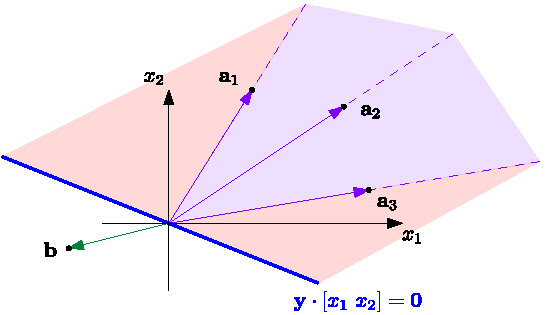
\includegraphics[width=0.6\textwidth ]{images/Farkas.pdf}
    }
    \caption{Secondo il lemma di Farkas, si può descrivere un iperpiano $\y^T\x=\mathbf 0$ che divide il vettore $\bb$ dal cono convesso.}
\end{figure}

Presenteremo adesso alcuni richiami di analisi sugli insiemi reali necessari per la dimostrazione della versione geometrica del lemma di Farkas.\bigskip 

$Z\subseteq \R^n$ è un insieme \textit{aperto} se per ogni $\x\in Z$, esiste una palla $B_\epsilon(\x)$ centrata in $\x$ di raggio $\epsilon$ (arbitrario) che è contenuta in $Z$. Si ricordi che \begin{itemize}
    \item l'unione di due insiemi aperti è un'insieme aperto  
    \item l'intersezione di due insiemi aperti è un'insieme aperto  
\end{itemize}

\begin{lemma2}\label{fatto}
    se $f$ è una funzione continua e biettiva su $\R^n$ e $U\subseteq \R^n$ è aperto, l'insieme $f(U)$ è aperto. Se $Z\subset \R^n$ è un'insieme chiuso e limitato, allora $f(Z)$ è un'insieme chiuso.  
\end{lemma2}
\begin{definizione}
    Dati $n$ punti $\mathbf a_1,\mathbf a_2,\dots, \mathbf a_n \in \R^m$, il cono convesso generato da questi è \textbf{primitivo} se $\mathbf a_1,\mathbf a_2,\dots, \mathbf a_n$ sono linearmente indipendenti.
\end{definizione}

La dimostrazione del lemma \ref{Farkas_geometrico} consiste nella dimostrazione di 5 proposizioni.
\begin{proposizione}\label{farkas_punto1}
    Se $C$ è un cono convesso, allora $C$ è l'unione di un'insieme finito di coni primitivi.
\end{proposizione}
\textit{Dimostrazione:} Siano  $\mathbf a_1,\mathbf a_2,\dots, \mathbf a_n \in \R^m$ i punti che generano $C$, sia 
$$ \mathcal I = \{ I\subseteq \{1,\dots,n\} \text{ t.c. } \{\mathbf a_i \ i\in I\} \text{ sono linearmente indipendenti}\}$$
$\mathcal I$ è un sotto-insieme dell'insieme potenza di $\{1,\dots n\}$, ha quindi cardinalità $|\mathcal I|\le 2^n$. Si denota $C_I$ il cono primitivo generato dall'insieme $\{\mathbf a_i \ i\in I\}$ con $I\in\mathcal I$. Si vuole mostrare che 
$$ 
\bigcup_{I\in\mathcal I}C_I=C
$$
Sia $\x$ un elemento fissato di $C$
$$ \x=\sum \alpha_i\mathbf a_i, \ \ \ \ \alpha_i\ge 0$$
Sia $\x$ definito come segue: $\x$ è l'elemento cha massimizza il numero di coefficienti $\alpha_i$ uguali a zero, quindi ogni altro elemento di $C$ è una combinazione lineare di $\mathbf a_i$ che ha un numero di  coefficienti nulli minore del numero di coefficienti nulli di $\x$.

Sia $I=\{i : \mathbf a_i>\mathbf 0\}$, si pone per assurdo che i vettori $\mathbf a_i$ con $i\in I$ non sono linearmente indipendenti, ossia 
\begin{equation}
    \exists\beta_i\in\R \ \ \ \text{ t.c. } \ \ \ \sum_{i\in I}\beta_i\mathbf a_i = \mathbf 0
\end{equation}
Si consideri il particolare coefficiente 
$$ \alpha_i-t\beta_i$$
per qualche $t\in \R$, per definizione, $\alpha_i>0$, scegliendo un valore di $t$ molto piccolo, $\alpha_i-t\beta_i>0$, se $t$ cresce indefinitamente, ad un certo punto $\alpha_i-t\beta_i$ diverrà negativo.
Si sceglie $t=\frac{\alpha_j}{\beta_j}$ con $j$ l'indice che minimizza fra tutti il valore assoluto $$ |\frac{\alpha_j}{\beta_j}|$$
il vettore 
$$ \x^*=\sum_{i\in I}(\alpha_i-t\beta_i)\mathbf a_i=\sum_{i\in I}(\alpha_i-\frac{\alpha_j}{\beta_j}\beta_i)\mathbf a_i$$
è per definizione un elemento del cono convesso $C$ dato che, per la specifica scelta di $t$, si ha che $(\alpha_i-t\beta_i)\ge 0$ per ogni $i\in I$, inoltre il vettore si può riscrivere 
\begin{eqnarray*}\x^*=
\sum_{i\in I}\alpha_i\mathbf a_i + t\sum_{i\in I}\beta\mathbf a_i =\\ \x+ t\sum_{i\in I}\beta\mathbf a_i
\end{eqnarray*}
La scelta di $t$ rende uno dei coefficienti $(\alpha_i-t\beta_i)$ uguali a zero, quindi $\x^*$ ha un coefficiente nullo in più rispetto ad $\x$, ma questo per definizione massimizzava il numero di coefficienti nulli, è quindi impossibile che l'assunzione che i vettori $\mathbf a_i$ con $i\in I$ non siano linearmente indipendenti sia vera, quindi 
$\mathbf a_i$ con $i\in I$ sono linearmente indipendenti, allora $\x$ è nel cono primitivo $C_I$, quindi $ 
\bigcup_{I\in\mathcal I}C_I=C
$.\hfill$\blacksquare$

\begin{proposizione}\label{farkas_punto2}
    Ogni cono primitivo è un'insieme chiuso.
\end{proposizione}
\textit{Dimostrazione}: Sia $C_I$ un cono primitivo generato da $\mathbf{a}_i$ (linearmente indipendenti) con $i\in I$. si consideri la base canonica di $\R^n$
$$ \mathbf e_1,\mathbf e_2\dots,\mathbf e_n=
\begin{bmatrix}
    1\\0\\\vdots\\0
\end{bmatrix},\begin{bmatrix}
    0\\1\\\vdots\\0
\end{bmatrix}\dots,\begin{bmatrix}
    0\\0\\\vdots\\1
\end{bmatrix}$$
dove $\mathbf e_i$ è il vettore composto da tutti zeri fatta eccezione per l'$i$-esima componente che è uguale ad $1$. Sia $\bar C$ il cono convesso generato da $ \mathbf e_1\dots,\mathbf e_n$, questo è chiuso perché è l'intersezione di un'insieme finito di mezzi spazi. Si consideri la funzione $f:\R^n\rightarrow\R^n$ definita come segue 
$$f([x_i \ : \ i\in I]^T)=\sum_{i\in I}x_i\mathbf a_i$$
essendo che $\mathbf{a}_i, \ i\in I$  sono linearmente indipendenti, $f$ è continua ed iniettiva, ma allora, essendo che $f(\bar C)=C_I$, per il lemma \ref{fatto}, $C_I$ è chiuso.
\begin{proposizione}\label{farkas_punto3}
    Ogni cono convesso è un'insieme chiuso. La dimostrazione è banale e segue dalle proposizioni \ref{farkas_punto1} e \ref{farkas_punto2}.
\end{proposizione}
\begin{proposizione}\label{farkas_punto4}
    Se $X\subset \R^n$ è un'insieme chiuso e $\bb\notin X$, allora esiste un punto $\mathbf z\in X$ che minimizza la distanza euclidea con $\bb$, ossia è il \textg{più vicino } a $\bb$.
\end{proposizione}
\textit{Dimostrazione}: Sia $\x$ un punto in $X$, si consideri la sfera $B_\varepsilon(\bb)$ centrata in $\bb$ di raggio 
$$ \varepsilon = \|\bb-\x\|$$
$B_\varepsilon(\bb)$ è un'insieme chiuso, l'insieme $B_\varepsilon(\bb)\cap X$ è chiuso e limitato, si consideri la funzione $f:\R^n\rightarrow\R$ definita come segue
$$ f(\y)=\|\bb-\y\|$$
$f$ è continua in $B_\varepsilon(\bb)\cap X$ ed ha un minimo, tale punto è proprio il punto più vicino a $\bb$.
\begin{proposizione}\label{farkas_punto5}
    Se $C$ è un cono convesso di $\R^n$ e $\bb\notin C$, allora esiste $\mathbf z\in C$ tale che $\mathbf z$ è l'elemento di $C$ più vicino a $\bb$. La dimostrazione segue dalle proposizioni \ref{farkas_punto3} e \ref{farkas_punto4}.
\end{proposizione}
\textg{Dimostrazione (Lemma \ref{Farkas_geometrico})}: Sia $C$ il cono convesso, si assume che $\bb\notin C$, per la proposizione \label{farkas_punto5} esiste un punto $\mathbf z$ nel cono che è il più vicino a $\bb$.

\begin{figure}[h]
    \centering{
        \includegraphics[width=0.45\textwidth ]{images/dim_Farkas.eps}
    }
    \caption{$\mathbf z$ è il punto in $C$ più vicino a $\bb$}
\end{figure}

Si considera l'iperpiano 
$$H=\{\y\in\R^m \ : \ (\mathbf z-\bb)^T\y=0\} $$
Si noti che $(\mathbf z-\bb)$ è ortogonale a $\mathbf z$, se così non fosse, esisterebbe un punto in $C$ più vicino a $\bb$. Si vuole mostrare che $(\mathbf z-\bb)^T\bb<0$\begin{eqnarray}
    \mathbf z - \bb \ne 0 \implies (\mathbf z - \bb)^T(\mathbf z - \bb)>0\implies \\ 
    (\mathbf z - \bb)^T\mathbf z - (\mathbf z - \bb)^T\bb >0
\end{eqnarray}
ma $(\mathbf z - \bb)^T\mathbf z =0$ data l'ortogonalità, quindi \begin{eqnarray}
    (\mathbf z - \bb)^T\mathbf z - (\mathbf z - \bb)^T\bb >0\implies\\ 
    - (\mathbf z - \bb)^T\bb >0\implies  (\mathbf z - \bb)^T\bb<0
\end{eqnarray}

Questo dimostra che $\bb$ non si trova sull'iperpiano ma su uno dei due mezzi-spazi definiti da esso. Inoltre, per ogni $\mathbf a_i$ si ha che 
$$ (\mathbf z -\bb)^T\mathbf a_i=\|\mathbf z -\bb\|\cdot \|\mathbf a_i\|\cos\theta$$
ed ogni termine di tale prodotto è positivo, quindi $ (\mathbf z -\bb)^T\mathbf a_i>0$, allora i vettori $\mathbf a_i$, e conseguentemente tutto il cono convesso da loro generato, si trovano sull'altra metà di spazio definita da $H$.\hfill$\blacksquare$
\section{Il Teorema degli Slack Complementari}
Si consideri una coppia $P,D$ di problemi primario-duale\begin{equation}\label{PD}
P=\begin{cases}
    \max \mathbf c^T\mathbf x\\ 
    A\mathbf x \le \mathbf b \\ 
    \mathbf x \ge 0 
\end{cases} \ \ \ \ D=
\begin{cases}
    \min \mathbf b^T\mathbf y\\ 
    A^T\mathbf y \ge \mathbf c \\ 
    \mathbf y \ge 0 
\end{cases}\end{equation}
I vincoli in $P$ corrispondono a variabili in $D$, e vincoli in $D$ corrispondono a variabili in $P$. Data una soluzione $\x^*$, un vincolo 
$$ x_1a_{j1}+\dots x_na_{jn}\le b_j$$
si dice \textbf{slack} o \textbf{residuo} se 
$$ x^*_1a_{j1}+\dots x^*_na_{jn}< b_j$$
Ossia il vincolo soddisfa la disuguaglianza in maniera \textit{stretta}, $A_j^T\x^*$ è strettamente minore di $b_j$. Se invece 
$$ x^*_1a_{j1}+\dots x^*_na_{jn} = b_j$$
il vincolo per $\x^*$ si dice \textbf{binding} o \textbf{saturo}. Tale denotazione si adotta anche ai vincoli del tipo $\x\ge \mathbf 0$, infatti se 
$$ x^*_i>0$$
la variabile $x_i^*$ è slack, altrimenti se 
$$ x^*_i=0$$
è binding. In tale contesto, il termine slack non è da confondere con le variabili slack che si aggiungono ad un programma lineare per farlo passare dalla forma canonica alla forma d'equazione. Si noti che la \textit{slackness} di ogni variabile è riferita ad una specifica soluzione.\bigskip 

Il seguente teorema è fondamentale, descrive la relazione fra vincoli di un problema e variabili del suo duale nei termini della \textit{slackness}.
\begin{teorema}\label{complementary_slackness}
    \textbf{(Complementary Slackness)} Siano $P,D$ una coppia di problemi primario-duale definiti come in \ref{PD}, entrambi ammissibili e limitati, sia $\x^*$ la soluzione ottimale per $P$, e $\y^*$ la soluzione ottimale per $D$, si ha che \begin{enumerate}
        \item Se $x^*_i>0$, ossia la variabile $x_i$ è slack per $\x^*$, allora il vincolo $i$-esimo di $D$ per $\y^*$ è binding.
        \item Se il $j$-esimo vincolo di $P$ è slack per $\x^*$, allora $y^*_j=0$, ossia
        la variabile $y_j$ è binding per $\y^*$.
        \item Se $y^*_j>0$, ossia la variabile $y_i$ è slack per $\y^*$, allora il vincolo $j$-esimo di $P$ per $\x^*$ è binding.
        \item Se l'$i$-esimo vincolo di $D$ è slack per $\y^*$, allora $x^*_i=0$, ossia
        la variabile $x_i$ è binding per $\x^*$.
    \end{enumerate}
\end{teorema}
\textit{Dimostrazione}: per ogni soluzione ammissibile $\bar\x$ per $P$, e $\bar\y$ per $D$ si ha 
$$ A\bar\x\le \bb$$
moltiplicando tutto per $\bar\y^T$
$$ \bar\y^TA\bar\x\le \bar\y^T\bb$$
Analogamente, essendo 
$$ A^T\bar\y\ge \bc$$
si ha 
$$ A^T\bar\y\bar\x\ge \bc^T\bar\x$$
Quindi è valida la seguente\begin{equation}
    \bc^T\bar\x\le\bar\y^TA\bar\x\le\bb^T\bar\y
\end{equation}
essendo che duale e primario hanno lo stesso ottimo 
$$ \bc^T\x^*=\bb^T\y^*$$
si ha che 
\begin{equation}
     \bc^T\x^*={\y^*}^TA\x^*=\bb^T\y^*
\end{equation}
Considerando la prima disuguaglianza \begin{eqnarray}
     \bc^T\x^*={\y^*}^TA\x^*\implies \\
      \bc^T\x^*-{\y^*}^TA\x^*=0\implies \\
      (\bc^T-{\y^*}^TA)\x^*=0 \implies \\ \label{slackness_teo}
      \sum_{i=1}^n(c_i-{\y^*}^TA_i)x^*_i=0
\end{eqnarray}
ma $(c_i-{\y^*}^TA_i)$ è minore o uguale di zero per ogni $i$, dato il vincolo $A^T\y\ge\bc$, e $x_i^*$ è maggiore o uguale a zero per ogni $i$, dato il vincolo $\x\ge 0$.\begin{itemize}
    \item ogni termine della sommatoria \ref{slackness_teo} è il prodotto fra un numero maggiore o uguale a zero per uno minore o uguale a zero.
    \item la somma totale è zero 
    \item ogni prodotto $(c_i-{\y^*}^TA_i)x^*_i$ della sommatoria è quindi uguale a zero
\end{itemize}
Quindi $x_i^*>0$ (l'$i$-esima variabile di $P$ è slack), necessariamente $c_i-{\y^*}^TA_i=0\implies {\y^*}^TA_i=c_i$ (l'$i$-esimo vincolo di $D$ è binding). 

Analogamente, se $c_i-{\y^*}^TA_i<0\implies {\y^*}^TA_i<c_i$ (l'$i$-esimo vincolo di $D$ è slack), necessariamente $x_i^*=0$ (l'$i$-esima variabile di $P$ è binding). Quindi i punti \textit{(1)} e \textit{(4)} del teorema sono dimostrati, i restanti punti possono essere dimostrati in maniera analoga.\hfill$\blacksquare$
\subsection{Alcune Applicazioni}
Il teorema \ref{complementary_slackness} può essere utilizzato per trovare la soluzione di un programma lineare, data una soluzione per il suo duale.
Siano $P$ e $D$ una coppia di problemi primario-duale, sia $\x^*$ la soluzione ottimale per $P$, se $x_i^*>0$ allora l'$i$-esimo vincolo di $D$ è binding, quindi in forma di equazione, inoltre, in base a quali vincoli di $P$ sono binding, si possono porre le variabili della soluzione $\y^*$ di $D$ uguali a zero, costruendo un sistema di $k$ equazioni in $k$ variabili.\bigskip 

\textit{Esempio}: Si consideri la seguente coppia di problemi primario duale: 
\begin{equation}
    P=\begin{cases}
        \max \  2x_1+4x_2+3x_3+x_4\\
        3x_1+x_2+x_3+4x_4\le 12\\ 
        x_1-3x_2+2x_3+3x_4\le 7\\ 
        2x_1+x_2+3x_3-x_4\le 10\\ 
        x_1,x_2,x_3,x_4\ge 0
    \end{cases}
    D=\begin{cases}
        \min \ 12y_1+7y_2+10y_3\\ 
        3y_1+y_2+2y_3\ge2\\
        y_1-3y_2+y_3\ge 4\\ 
        y_1+2y_2+3y_3\ge 3 \\ 
        4y_1+3y_2-y_3\ge 1\\ 
        y_1,y_2,y_3 \ge 0 
    \end{cases}
\end{equation}
Si consideri la soluzione ottimale $\x^*=\begin{bmatrix}
    0&10.4&0&0.4
\end{bmatrix}^T$ per $P$, dato che $x_2^*,x_4^*>0$, per il teorema \ref{complementary_slackness} è vero che, se $\y^*$ è la soluzione ottimale per $D$ si ha 
\begin{eqnarray*}
y^*_1-3y^*_2+y^*_3 = 4\\ 
4y^*_1+3y^*_2-y^*_3 = 1
\end{eqnarray*}
Inoltre si noti come il secondo vincolo di $P$ per $\x^*$ è slack
\begin{eqnarray*}
     x_1^*-3x_2^*+2x_3^*+3x_4^*=\\
    -3\cdot 10.4+3\cdot 0.4 = -28.6 < 7
\end{eqnarray*}
Quindi $y_2^*=0$, si ha il seguente sistema di equazioni 
$$ 
\begin{cases}
y^*_1-3y^*_2+y^*_3 = 4\\ 
4y^*_1+3y^*_2-y^*_3 = 1\\ 
y_2^*=0
\end{cases}\implies 
\begin{cases}
y^*_1+y^*_3 = 4\\ 
4y^*_1-y^*_3 = 1\\ 
y_2^*=0
\end{cases}\implies \y^*=\begin{bmatrix}
    1&0&3
\end{bmatrix}^T
$$
Un'altra possibilità è quella di usare il teorema \ref{complementary_slackness} per verificare che una data soluzione ammissibile sia ottimale. Proseguendo in tale maniera\begin{enumerate}
    \item Data una soluzione $\x^*$ da verificare, si assume che sia ottimale 
    \item Si calcola tramite il teorema \ref{complementary_slackness} la soluzione $\y^*$ ottimale per il suo duale 
    \item Si verifica che le due soluzioni assumano lo stesso valore sulle funzioni obiettivo dei due problemi
\end{enumerate}

si consideri la seguente coppia di problemi primario duale\begin{equation}
    P=\begin{cases}
        \max \ 2x_1+16x_2+12x_3 \\ 
        2x_1+x_2-x_3\le 3\\ 
        -3x_1+8x_2+2x_3\le 12 \\ 
        x_1,x_2,x_3\ge 0
    \end{cases}
    D=\begin{cases}
        \min \ 3y_1+12y_2\\ 
        2y_1-3y_2\ge 2 \\ 
        y_1+8y_2\ge 16\\ 
        -y_1+2y_2\ge 12 \\ 
        y_1,y_2\ge 0
    \end{cases}
\end{equation}
Si vuole verificare che $\x^*=\begin{bmatrix}
    6&0&12
\end{bmatrix}^T$ sia ottimale, si assume che lo sia e si calcola la soluzione ottimale per $D$.\begin{itemize}
    \item Si noti come entrambi i vincoli di $P$ per $\x^*$ sono slack, quindi $y^*_1,y_2^*=0$
\end{itemize}
la soluzione ottimale per $D$ dovrebbe essere $\y^*=\begin{bmatrix}
    0&0
\end{bmatrix}^T$, ma questa non soddisfa i vincoli di $D$, quindi è impossibile che $\x^*$ sia ottimale.

\chapter{Metodi Polinomiali per la Risoluzione di un LP}
Esiste uno specifico poliedro definito su $\R^n$ che soddisfa le seguenti \begin{itemize}
    \item il poliedro è definito da $3n$ equazioni 
    \item esiste un cammino sui vertici di lunghezza $2^n-1$ che collega due punti
\end{itemize}
\begin{figure}[h]
    \centering{
        \includegraphics[width=0.7\textwidth ]{images/Klee-Minty-polyhedron.eps}
    }
\end{figure}

Tale risultato è stato dimostrato da  \textit{Klee} e \textit{Minty}, l'implicazione è chiara, nel caso peggiore il metodo del simplesso esegue un numero di passi esponenziali nella dimensione dell'input. È stato poi dimostrato che se venissero ordinate in maniera casuale le $n$ variabili del problema, per poi applicare la regola di Bland, il valore atteso del numero di pivot controllati nell'esecuzione sarebbe $\exp(C\sqrt{n\ln{(n)}})$, dove $C$ è una data costante.
\begin{definizione}
    Il \textbf{diametro} di un poliedro è la massima distanza (in termini di cammino sui vertici) fra due vertici qualsiasi del poliedro.
\end{definizione}
\textbf{Congettura di Hirsh} ogni poliedro in $\R^n$ definito da $cn$ vincoli ($c$ costante) ha un diametro minore o uguale a $n^c$.\bigskip 

Esistono degli algoritmi polinomiali per la risoluzione di un programma lineare, è necessario descrivere prima quale sia la dimensione dell'input di un LP. Un programma lineare è descritto da una matrice e due vettori 
$$ A\in Mat(m\times n),\bb\in \R^m,\bc\in\R^n$$
Quanti bit servono per descrivere tali elementi? Per descrivere un singolo numero intero $\alpha$, sono necessari 
$ \lceil \log_2(\alpha)+1 \rceil $ bit, si denota tale grandezza $\bra{\alpha}$.\begin{quote}
    \textbf{assunzione}: Tutte le componenti di $A,\bb$ e $\bc$ sono numeri razionali
\end{quote}
Tale assunzione è fondamentale per far si che i numeri di  $A,\bb$ e $\bc$ si possano rappresentare con un numero finito di bit. Un qualsiasi numero razionale $\frac{p}{q}$ si può rappresentare come frazione di due numeri interi, quindi
$$ \bra{\frac{p}{q}}=\bra p+\bra q$$
le dimensioni di un vettore $\x\in\R^d$ si esprimono come somma delle dimensioni dei suoi componenti 
$$ \bra\x=\sum_{i=1}^d\bra{x_i}$$
analogamente, si descrivono le dimensioni della matrice $A$ come segue 
$$\bra A=\sum_{i=1}^n\sum_{j=1}^m\bra{A_{ij}}$$
dato un programma lineare $P$ in forma canonica, la dimensione del problema è
$$ \bra P = \bra A +\bra\bb+\bra\bc$$
L'algoritmo seguente farà un numero polinomiale in $\bra P$ di operazioni bit a bit. Non descriveremo un algoritmo che fa un numero di operazioni polinomiale in $n,m$, in quel caso, sarebbe \textbf{fortemente polinomiale}.
\section{Metodo degli Ellissoidi}
Sia $B^n$ la palla unitaria di $\R^n$
$$ B^n=\{\x\in\R^n \ : \ \|\x\|\le 1\}$$
\begin{definizione}
    Data una matrice $M$ non singolare ed un vettore $\bs$ (detto centro), un'\textbf{ellissoide}  è il seguente insieme 
    $$ E=\{M\x+\bs \ : \ \x\in B^n\}$$
\end{definizione}
geometricamente, un'ellissoide è una sfera che è stata stirata dall'applicazione lineare $M$ e centrata in $\bs$.

\begin{figure}[h]
    \centering{
        \includegraphics[width=1\textwidth ]{images/ellissoide.eps}
    }
\end{figure}

Un ellissoide $E$ si può definire anche in maniera differente 
$$ E=\{\y\in\R^n \ : \ M^{-1}(\y-\bs)\in B^n\} = $$
$$ E=\{\y\in\R^n \ : \ (\y-\bs)^T {M^{-1}}^TM^{-1}(\y-\bs) \le 1\} = $$
$$ E=\{\y\in\R^n \ : \ (\y-\bs)^TQ(\y-\bs) \le 1\}  $$
dove $Q={M^{-1}}^TM^{-1}$ è una matrice quadrata \textbf{positiva semi-definita}, ossia $$ \x^TQ\x>0, \forall \x$$

\pgfplotsset{compat=1.15}

\begin{figure}[h!]
    \centering
\begin{tikzpicture}
\begin{axis}
[view={135}{20},colormap={blue}{
            color=(blue) color=(blue)
        },
axis lines=center,axis on top,
ticks=none,set layers=default,axis equal,
xlabel={$x$}, ylabel={$y$}, zlabel={$z$},
xlabel style={anchor=south east},
ylabel style={anchor=south west},
zlabel style={anchor=south west},
enlargelimits,
tick align=inside,
domain=0:2.00,
samples=15, 
z buffer=sort,
]
\addplot3 [surf,draw=blue!30,fill=white,domain=-1:1,samples=15,
domain y=00:180] ({x},{-2*cos(y)*sqrt(1-x^2)},{-sin(y)*sqrt(1-x^2)});
\addplot3 [surf,draw=blue!30,fill=white,domain=-1:1,
domain y=0:180,on layer=axis foreground] ({x},{2*cos(y)*sqrt(1-x^2)},{sin(y)*sqrt(1-x^2)});
\end{axis}
\end{tikzpicture}
\caption{ellissoide in $\R^3$}
\end{figure}

\begin{teorema}
    $Q$ è una matrice positiva semi-definita se e solo se esiste una matrice $M$ non singolare tale che $$ Q=MM^T$$ 
\end{teorema}
\textbf{Corollario}: $E\subset \R^n$ è un ellissoide se e solo se esiste una matrice positiva semi-definita $Q$ ed un vettore $\bs\in\R^n$ tale che 
$$ E=\{\y\in\R^n \ : \ (\y-\bs)^TQ(\y-\bs) \le 1\}  $$
Il metodo degli ellissoidi non risolverà direttamente un programma lineare, ma si occuperà di verificare se un dato poliedro è o non è vuoto, è stato già dimostrato in precedenza che i due problemi sono equivalenti. Una descrizione iniziale del funzionamento dell'algoritmo è la seguente\begin{itemize}
    \item L'algoritmo prende come input un poliedro $P$ descritto da una matrice $A$ ed un vettore $\bb$ 
    $$P=\{\x \ : \ A\x\le \bb, \ \ \x\ge \mathbf 0\} $$
    e due numeri razionali $R,\varepsilon$, l'assunzione è che $P$ sia contenuto interamente nella palla $B^n(\mathbf 0,R)$ di raggio $R$ centrata nell'origine.
    $$ B^n(\mathbf 0,R)=\{\x\in\R^n \ : \ \|\x\|\le R\}$$
    \item l'algoritmo genera una serie di $t$ ellissoidi $E_1,E_2\dots, E_t$ tali che 
    $P\subset E_i$ per ogni $i$
    \item l'algoritmo termina restituendo una delle seguenti risposte \begin{itemize}
        \item è stato trovato un punto in $P$, ed è il centro di $E_t$
        \item il volume di $E_t$ è minore di $\varepsilon$
    \end{itemize}
\end{itemize}

\begin{figure}[h]
    \centering{
        \includegraphics[width=0.35\textwidth ]{images/assunzione_ellissoidi.eps}
    }
    \caption{l'assunzione che il poliedro sia contenuto nella palla di raggio $R$}
\end{figure}

In particolare, se l'algoritmo non trova in punto in $P$, restituisce un \textit{certificato} che il poliedro non contiene una palla di raggio $\varepsilon$.\bigskip 

Nell'algoritmo, l'ellissoide iniziale $E_0$ è proprio $B^n(\mathbf 0,R)$, denotiamo $\bs_i$ il centro dell'$i$-esimo ellissoide, in tal caso, $\bs_0=\mathbf 0$. Si assuma di essere nel $k$-esimo passo, e si a disposizione l'ellissoide $E_k$ centrato in $\bs_k$. Si verifica che $\bs_k$ sia un'elemento di $P$ 
$$ A\bs_k\le \bb$$
se ciò dovesse essere vero, si restituirebbe $\bs_k$, altrimenti, si avrebbe un vincolo che tale punto non soddisfa 
$$ A_i^T\bs_k>b_i \ \ \ \text{ per qualche } i$$
Il vincolo $i$-esimo definisce un iperpiano, e a sua volta un mezzo spazio 
$$ \{\x \ : \ A_i^T\x\le b_i\}$$
$\bs_k$ violando il vincolo, non si trova nel mezzo-spazio appena definito.\begin{center}
    \includegraphics[width=0.5\textwidth ]{images/taglio_ellissoide.eps}
\end{center}
Si considera l'iperpiano parallelo a $ \{\x \ : \ A_i^T\x= b_i\}$ ma passante per $\bs_k$, ossia quello che genera il mezzo spazio 
$$\{\y \ : \ A_i^T\y\le A_i^T\bs_k\}$$
e si considera l'insieme $H_k$ che è intersezione di tale mezzo spazio e $E_k$
$$ H_k=E_k\cap \{\y \ : \ A_i^T\y\le A_i^T\bs_k\}$$
\begin{center}
    \includegraphics[width=0.55\textwidth ]{images/taglio_ellissoide2.eps}
\end{center}
Si sceglie il prossimo ellissoide $E_{k+1}$ come il più piccolo ellissoide contenente $H_k$, e si avrà che $P\subset E_{k+1}$. La seguente proposizione non verrà dimostrata, ma è fondamentale per la descrizione dell'algoritmo.
\begin{proposizione}
    Dato l'ellissoide $E_k\subset \R^n$ descritto da un centro  $\bs_k$ che viola l'$i$-esimo vincolo di $A$ $$ A_i^T\bs_k>b_i$$
    e $Q_k$ matrice positiva semi-definita, Il più piccolo ellissoide contenete 
    $$ H_k=E_k\cap \{\y \ : \ A_i^T\y\le A_i^T\bs_k\}$$ 
    è univocamente definito dal centro $\bs_{k+1}$ e dalla matrice $Q_{k+1}$ come segue
    \begin{eqnarray}
        \bs_{k+1}=\bs_k-\frac{1}{n-1}\frac{1}{\sqrt{A_iQ_kA_i^T}}Q_kA_i^T\\ 
        Q_{k+1}=\frac{n^2}{n^2+1}\Big(
        Q_k-\frac{2}{n+1}\frac{Q_kA_i^TA_iQ_k}{A_iQ_kA_i^T}    
        \Big)
    \end{eqnarray}
\end{proposizione}
\noindent Il volume dell'ellissoide $E_k$ è l'integrale della funzione identità su di esso 
$$ \text{vol}(E_k)=\int_{E_k}d\x$$
e passando da un'ellissoide al successivo nell'algoritmo tale volume decresce di un valore costante 
$$ 
\frac{\text{vol}(E_{k+1})}{\text{vol}(E_{k})}\le e^{-\frac{1}{2n+2}}<1
$$
Durante la successione di ellissoidi, se il volume dell'ellissoide corrente è minore del volume della palla di raggio $\varepsilon$ dato in ingresso, l'algoritmo termina senza restituire una soluzione, garantendo però che $P$ non è contenuto nella palla di raggio $\varepsilon$.
\begin{proposizione}
    L'algoritmo termina in un numero di passi polinomiale in funzione di $\bra A+\bra \bb+\bra R+\bra \varepsilon$.
\end{proposizione}
\textit{Dimostrazione}:  Il volume di $E_0=B^n(\mathbf 0,R)$ è $c\cdot R^n$ per qualche costante $c$ che dipende da $n$, inoltre per ogni $k$ si ha 
$$ \text{vol}(E_k)\le \text{vol}(E_{k+1})e^{-\frac{k}{2n+2}}$$
se $k\ge n(2n+2)\ln(\frac{R}{\varepsilon})$ si ha che 
\begin{eqnarray}
    \text{vol}(E_k)\le cR^n\cdot e^{\lceil n\cdot\ln(\frac{R}{\varepsilon}) \rceil}\\ 
    cR^n\cdot e^{\lceil n\cdot\ln(\frac{R}{\varepsilon}) \rceil}=\frac{cR^n}e^{-\frac{R^n}{\varepsilon^n}}\le \varepsilon
\end{eqnarray}
Quindi $\lceil n(2n+2)\ln(\frac{R}{\varepsilon})\rceil$ è il massimo numero di passi del metodo degli ellissoidi, ed è polinomiale in $\bra A+\bra \bb+\bra R+\bra \varepsilon$.\hfill$\blacksquare$
\subsection{Tecnicalità Implementative}
Ci sono alcune criticità nel metodo degli ellissoidi, il calcolo del centro dell'ellissoide successivo avviene considerando il termine 
$$ \bs_{k+1}=\bs_k-\frac{1}{n-1}\frac{1}{\sqrt{A_iQ_kA_i^T}}Q_kA_i^T$$
questo presenta una radice quadrata quindi viola l'assunzione che tutti i numeri rappresentati siano razionali, è necessario includere un'ulteriore argomento in input, $\varepsilon_2$ necessario per arrotondare $\bs_{k+1}$ in modo da far si che ogni sua componente sia un numero razionale. Vi è un'altro problema, come viene scelto il valore di $R$ iniziale per far si che la palla $B^n(\mathbf 0,R)$ contenga completamente il poliedro $P$?\bigskip 
Siano $\varphi$ e $l$ due valori definiti come segue\begin{equation}
    \varphi = \bra A +\bra\bb \ \ \ \ \ \ \ l=2^\varphi
\end{equation}
\begin{proposizione}
    Assumendo che ogni numero considerato sia razionale, il problema $A\x\le \bb, \ \x\ge \mathbf 0$ ha una soluzione se e solo se il problema$$ \begin{cases}
        A\x\le \bb\\ \x\ge \mathbf 0\\ 
        x_i\le l, \ \ \forall i 
    \end{cases}$$
    ha soluzione.
\end{proposizione}
\textit{Dimostrazione}: sia $\x^*$ una soluzione per il problema $A\x\le \bb, \ \x\ge \mathbf 0$, essendo $\x^*$ una soluzione ad un sistema di equazioni nei termini di $A$ e $\bb$, il numero di bit per rappresentare ogni $x_i^*$ è al più $\bra A +\bra \bb=\varphi $, quindi $x_i^*\le 2^\varphi = l$. \hfill$\blacksquare$

Quindi, scegliendo $R=l$, si ha la certezza che ogni possibile punto del poliedro sia contenuto nella palla $B^n(\mathbf 0,l)$.\bigskip

Vi è un'ultima tecnicalità da considerare, l'algoritmo potrebbe terminare senza restituire un punto in $P$ anche se quest'ultimo è non vuoto, dato che termina appena l'ellissoide $k$-esimo considerato ha un volume minore del volume della palla di raggio $\varepsilon$, e l'unica certezza che si ha da tale risultato è che il poliedro $P$ non contiene una palla di raggio $\varepsilon$.

Si definiscono \begin{eqnarray*}
    \eta  = 2^{-5\varphi}\\ 
    \mathbf z = \begin{bmatrix}
        \eta&\eta&\dots &\eta
    \end{bmatrix}^T\in\R^n
\end{eqnarray*}
e si sceglie $\varepsilon=2^{-6\varphi}$. Ciò è funzionale dato che il sistema $$A\x\le\bb$$ ha soluzione se e solo se il sistema $$A\x\le\bb+\mathbf z$$
ha soluzione, in tal caso l'insieme delle soluzioni ammissibili contiene necessariamente una palla di raggio $\varepsilon$.

In conclusione, per verificare che un poliedro 
$$ P=\{\x \ : \ A\x\le\bb, \ \ \x\ge\mathbf 0\}$$
sia o non sia vuoto, è sufficiente eseguire il metodo degli ellissoidi sul poliedro derivato 
$$ P'=\{\x \ : \ A\x\le\bb+\mathbf z, \ \ -l\le\x\le l\}$$
Se l'algoritmo restituisce un punto, allora $P$ non è vuoto, altrimenti si ha la certezza che $P$ sia vuoto. Tale metodo è polinomiale nelle dimensioni di $\bra A+\bra\bb$.
\section{Accenno al Metodo dei Punti Interni}
Il metodo degli ellissoidi non si presta ad essere efficiente se implementato su un calcolatore, nell'effettivo vengono utilizzate delle rivisitazioni del simplesso oppure il metodo dei punti interni, quest'ultimo consiste nello svilupparsi di un cammino di punti contenuti nel poliedro $P$, muovendosi verso un punto ottimale per la funzione obiettivo. Il problema dato in input è quindi un programma lineare del tipo \begin{eqnarray*}
    P=\{\x \ : \ A\x\le\bb, \ \ \x\ge\mathbf 0\}\\ 
    \max \ \bc^T\x \  \text{su } P
\end{eqnarray*}

\begin{figure}[h]
    \centering{
        \includegraphics[width=0.25\textwidth ]{images/interior_point.eps}
    }
\end{figure}

Si considera una funzione $f(\eta,\x)$ con $\x\in\R^n$ e $\eta\in[0,\infty)$ definita come segue\begin{equation}
    f(\eta,\x)=\bc^T\x+\eta\sum_{i=1}^n\ln(b_i-A_i\x)
\end{equation}
se $\eta=0$ allora $f(\eta,\x)=f(0,\x)=\bc^T\x$ è la funzione obiettivo, dal momento che il logaritmo non è definito in 0, $f(\eta,\x)$ non è definita sulla frontiera di $P$, ossia nei punti che annullano l'argomento del logaritmo $$ b_i=A_i\x\implies b_i-A_i\x=0$$
per ogni $\eta$ fissato, $f(\eta,\x)$ tende a $-\infty$ se $\x$ si avvicina alla frontiera di $P$, se $\eta$ tende a zero, $f(\eta,\x)$ tende a $\bc^T\x$.
\begin{proposizione}
    per ogni $\eta$ fissato, $f(\eta,\x)$ ha un'unico massimo in $P$.
\end{proposizione}
Senza entrare nel dettaglio, esistono dei metodi di ottimizzazione non lineare basati sui \textit{moltiplicatori di Lagrange} per la ricerca di un massimo di $f(\eta,\x)$, che porterà poi alla ricerca di un massimo per $\bc^T\x$ su $P$.

\chapter{Programmazione Intera}
La programmazione intera riguarda la soluzione di un programma lineare, con il vincolo ulteriore che la soluzione deve essere un vettore di numeri interi, il generico programma intero è il seguente\begin{equation}
    \begin{matrix}
        \max \bc^T\x\\ 
        A\x\le\bb\\ 
        \x\ge\mathbf 0\\ 
        \x\in\Z^n
    \end{matrix}
\end{equation}
Il noto \textbf{Knapsack Problem} è un classico esempio di problema che si può risolvere tramite la programmazione intera, vi è un'insieme di $n$ oggetti, $x_1,x_2\dots,x_n$, ad ogni oggetto $x_i$ è associato un valore $v_i$ ed un perso $w_i$, e si vuole trovare il sotto-insieme di oggetti $I$ che massimizza il valore complessivo$$ \sum_{i\in I}v_i$$ con il vincolo che il peso complessivo sia minore o uguale ad una certa costante $C$.
$$ \sum_{i\in I}w_i\le C$$
Il problema si modellizza considerando un vettore $\x$ che rappresenta gli oggetti, se $x_i=1$ allora l'$i$-esimo oggetto è considerato, altrimenti no$$ x_i=\begin{cases}
    1\text{ se }i\in I\\
    0\text{ altrimenti}
\end{cases}$$
sia $\mathbf v$ il vettore la cui $i$-esima componente $v_i$ è il valore dell'$i$-esimo oggetto, e $\mathbf w$ il vettore la cui $i$-esima componente $w_i$ è il peso dell'$i$-esimo oggetto. Il problema si modellizza come segue\begin{eqnarray*}
    \max \ \mathbf v^T\x\\ 
    \mathbf w^T\x\le C\\ 
    \x \in \{0,1\}^n
\end{eqnarray*}
\section{Inviluppo Convesso dei Punti Interi}
In questa sezione verrà presentato un metodo per la risoluzione di un programma intero. La programmazione intera è tipicamente NP-completa, non esiste quindi un algoritmo efficiente per risolvere un programma intero.\bigskip 

L'insieme dei vincoli di un programma intero definisce un poliedro proprio come quello definito da un programma lineare 
$$ P=\{\x\in\R^n \ : \ A\x\le\bb, \ \x\ge \mathbf 0\}$$
Si consideri $A$ come l'insieme dei punti interi contenuti in $P$
$$ A=\{\x\in\Z^n \ : \ \x\in P\}=\{\mathbf a_1,\mathbf a_2\dots,\mathbf a_k\}$$
è di \textit{fondamentale importanza} l'inviluppo convesso di $A$, che in tale contesto verrà indicato $P_I$, ossia l'insieme di tutte le combinazioni convesse di $A$
$$P_I =
     \Big\{\sum_{i=1}^k \alpha_i\mathbf{a}_i  \ \ : \ \ \alpha_i\ge 0 \ \forall i,\ \sum_{i=1}^n \alpha_i=1\Big\} $$

\begin{figure}[h]
    \centering{
        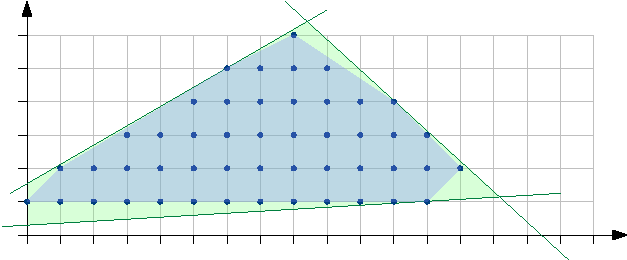
\includegraphics[width=0.7\textwidth ]{images/P_I.pdf}
    }
    \caption{In verde è rappresentato il poliedro definito dai vincoli, in blu l'inviluppo convesso dei suoi punti interi}
\end{figure}
\begin{proposizione}
    Sia $\mathbf u_1,\mathbf u_2\dots,\mathbf u_n$ un'insieme di punti in $\R^n$, e sia $H$ l'inviluppo convesso di tali punti. Se $\mathbf v$ è un vertice di $H$, allora $\mathbf v = \mathbf u_i$ per qualche $i$.
\end{proposizione}
\textit{Dimostrazione}: sia $H$ l'inviluppo convesso di $\mathbf u_1,\mathbf u_2\dots,\mathbf u_n$, e sia $\mathbf v$ un vertice di $H$, esiste quindi un iper-piano 
$$L=\{\x\in\R^n \ : \ \bc^T\x=\alpha\} $$contenente $\mathbf v$ tale per cui l'intero poliedro $H$ è contenuto in una delle due metà definite da $L$\begin{eqnarray*}
    \bc^T\mathbf v = \alpha\\ 
    \bc^T\x<\alpha, \forall \x\in H\backslash\{\mathbf v\}
\end{eqnarray*}

\begin{figure}[h]
    \centering{
        \includegraphics[width=0.3\textwidth ]{images/L_separa_H.eps}
    }
\end{figure}
Si pone per assurdo che $\mathbf u_i\ne\mathbf v$, ossia che 
$$ \mathbf v = \sum_{i=0}^n \beta_i\mathbf u_i, \ \ \ \sum_{i=1}^n\beta_i=1$$
$$ \exists j \text{ t.c. }0<\beta_j<1$$
Sia $j$ un fissato indice tale per cui $0<\beta_j<1$, si ha che 
$$ \mathbf v = \beta_j\mathbf u_j+\sum_{i\ne j}\beta_i\mathbf u_i$$
si consideri il seguente vettore 
$$ \sum_{i\ne j}\frac{\beta_i}{1-\beta_j}\mathbf u_i$$
tale vettore è contenuto in $H$ perché 
$$ \sum_{i\ne j}\beta_i=1-\beta_j\implies \sum_{i\ne j}\frac{\beta_i}{1-\beta_j}=\frac{1}{1-\beta_j}\sum_{i\ne j}\beta_i=1$$
si riscrive 
$$ \mathbf v = \beta_j\mathbf u_j+(1-\beta_j)\sum_{i\ne j}\frac{\beta_i}{1-\beta_j}\mathbf u_i$$
quindi 
$$ \bc^T\mathbf v=\bc^T\Big(
\beta_j\mathbf u_j+(1-\beta_j)\sum_{i\ne j}\frac{\beta_i}{1-\beta_j}\mathbf u_i    
\Big)$$
ricordando che $\bc^T\mathbf v = \alpha$
$$ \alpha=\bc^T\Big(
\beta_j\mathbf u_j+(1-\beta_j)\sum_{i\ne j}\frac{\beta_i}{1-\beta_j}\mathbf u_i    
\Big)$$
$$ \alpha=
\beta_j\bc^T\mathbf u_j+(1-\beta_j)\sum_{i\ne j}\frac{\beta_i}{1-\beta_j}\bc^T\mathbf u_i    
$$
essendo $$ \begin{matrix}
    \bc^T\mathbf u_j\le \alpha \\ 
    \bc^T\mathbf u_i \le \alpha, \ \forall i
\end{matrix}$$
si ha 
\begin{eqnarray*}
    \alpha \le \beta_j\alpha+(1-\beta_j)\sum_{i\ne j}\frac{\beta_i}{1-\beta_j}\alpha\\ 
    \alpha \le \beta_j\alpha+(1-\beta_j)\alpha=\alpha\implies\\ 
    \alpha = \bc^T\mathbf v = \beta_j\bc^T\mathbf u_j+\bc^T((1-\beta_j)\sum_{i\ne j}\frac{\beta_i}{1-\beta_j}\mathbf u_i)\le \alpha 
\end{eqnarray*}
serve specificatamente che $\bc^T\mathbf u_j=\alpha$, ma ciò è impossibile dato che solo il vertice $\mathbf v$ soddisfa tale condizione, vi è quindi una contraddizione.\hfill$\blacksquare$\bigskip 

\noindent Tale proposizione ha delle implicazioni favorevoli, sia $P$ un politopo, e $P_I$ l'inviluppo convesso dei punti interi di $P$, piuttosto che risolvere il programma intero 
\begin{eqnarray*}
    \max \bc^T\x\\ \x\in P \\ \x\in\Z^n
\end{eqnarray*}
è possibile risolvere il programma lineare
\begin{eqnarray*}
    \max \bc^T\x\\ \x\in P_I \\ \x\in\R^n
\end{eqnarray*}
Dato che la soluzione sarà un vertice di $P_I$, che sappiamo essere un vettore di numeri interi. Tale strategia permette di risolvere un programma intero, l'inviluppo convesso dei punti interi di un politopo è un'insieme generalmente più piccolo \begin{eqnarray*}
    P=\{\x \ : \ A\x\le\bb, \ \x\ge\mathbf 0\}\\ 
    P_I=\Big\{\x \ : \ \begin{bmatrix}
    A\\ \bar A
    \end{bmatrix}\x\le\begin{bmatrix}
    \bb\\ \bar \bb
    \end{bmatrix}, \ \x\ge\mathbf 0\Big\}
\end{eqnarray*}
L'inviluppo convesso $P_I$ è definito dai vincoli di $P$, con in aggiunta dei vincoli aggiuntivi $\bar A \x\le \bar \bb$. Dato un programma intero, com'è possibile trovare tali vincoli in modo da riformulare il problema come un programma lineare?
\subsection{Il Teorema di Gomory}
Si consideri il seguente programma intero \begin{equation}
    \begin{matrix}
        \max 5x_1+8x_2\\ x_1+x_2\le 6\\ 
        5x_1+9x_2\le45\\ 
        x_1,x_2\ge 0, \ x_1,x_2\in \Z
    \end{matrix}
\end{equation}
Si considera la sua versione rilassata in programma lineare (con aggiunta di variabili slack per renderlo in forma di equazione)
\begin{equation}
    \begin{matrix}
        \max 5x_1+8x_2\\ x_1+x_2+x_3= 6\\ 
        5x_1+9x_2+x_4=45\\ 
        x_1,x_2,x_3,x_4\ge 0
    \end{matrix}
\end{equation}
Si vuole risolvere il programma intero, si comincia risolvendo il programma lineare con il  metodo del simplesso, arrivando alla base $\mathcal B=\{1,2\}$ che fornisce il seguente tableau
\begin{center}
    \begin{tabular}{|l|l|}\hline 
        $x_1=\nicefrac{9}{4}-\nicefrac{9}{4}x_3-\nicefrac{1}{4}x_4$\\ 
        $x_2=\nicefrac{15}{4}+\nicefrac{5}{4}x_3-\nicefrac{1}{4}x_4$\\ 
        \hline 
        $z=\nicefrac{41}{4}-\nicefrac{5}{4}x_3-\nicefrac{3}{4}x_4$ \\\hline 
    \end{tabular}
\end{center}
La BFS ottimale trovata è un vettore contenente numeri razionali, quindi non valida come soluzione del programma intero, si noti però che la seconda equazione del tableau, ossia 
$$x_2=\nicefrac{15}{4}+\nicefrac{5}{4}x_3-\nicefrac{1}{4}x_4$$
esprime un vincolo che deve essere soddisfatto da ogni soluzione ammissibile, anche quelle intere:
\begin{eqnarray*}
    x_2=\frac{15}{4}+\frac{5}{4}x_3-\frac{1}{4}x_4\implies \\
    x_2-\frac{5}{4}x_3+\frac{1}{4}x_4=\frac{15}{4}\implies \\
    (1+0)x_2+(-2+\nicefrac{3}{4})x_3+(0+\nicefrac{1}{4})x_4=3+\nicefrac{3}{4}
\end{eqnarray*}
Il vincolo è stato espresso dividendo parti decimali ed intere dei coefficienti, se si assume che la soluzione è un vettore di numeri razionali, si ottiene il seguente vincolo, per qualche $k\in\Z^+$
$$ 
0x_2+\frac{3}{4}x_3+\frac{1}{4}x_4=k+\frac{3}{4}
$$
Che si può riscrivere come 
$$ 
\frac{3}{4}x_3+\frac{1}{4}x_4\ge \frac{3}{4}
$$
$$ 
-\frac{3}{4}x_3-\frac{1}{4}x_4\le -\frac{3}{4}
$$
Tale vincolo deve essere soddisfatto da ogni soluzione intera, si può quindi aggiungere al programma lineare, \textbf{tagliando} una porzione di politopo di soluzioni non intere.
\begin{center}
    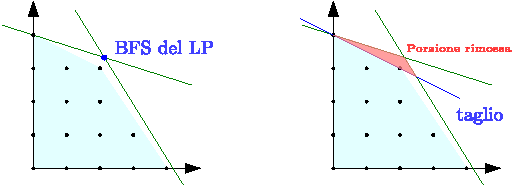
\includegraphics[width=0.7\textwidth ]{images/gomoryCut.pdf}
\end{center}
Vediamo la regola generale, quando si trova una soluzione ottimale non intera tramite il metodo del simplesso, nel tableau finale si avrà almeno un vincolo del tipo
$$ 
(a_1+f_1)x_1+(a_2+f_2)x_2+\dots+(a_n+f_n)x_n = a_0+f_0
$$
dove 
\begin{eqnarray*}
    a_i\in\Z\\ f_i \in [0,1)
\end{eqnarray*}
Considerando il vincolo 
$$ \sum_{i=1}^nf_i\ge f_0$$
Questo è detto il \textbf{taglio di Gomory} ed è soddisfatto da tutte le soluzioni intere del problema. Si può aggiungere tale vincolo (che esclude la soluzione ottimale non intera appena trovata) e ri-eseguire il metodo del simplesso.
\begin{teorema}
    Sia $P=\{\x \ : \ A\x=\bb, \ \x\ge\mathbf 0\}$ il poliedro di un LP e $\bar\x$ la BFS ottimale. Se $\bar \x$ non è un vettore di soli numeri interi, allora il taglio di Gomory applicato a $P$, definisce un nuovo poliedro $P'$ tale che \begin{itemize}
        \item $\bar\x\notin P'$ (taglia fuori la BFS)
        \item $\forall \x \in P\cap \Z^n, \ \ \x\in P'$ (preserva le soluzioni intere)
    \end{itemize}
\end{teorema}
\textit{Dimostrazione}: 
Si considera un riordinamento della matrice $A$, spostando le colonne inerenti alle variabili di base a sinistra, e le restanti a destra 
$$ A=\begin{bmatrix}
    A_{\mathcal B} \ | \ A_N
\end{bmatrix}$$
Si riordina poi anche il vettore delle variabili $\bar\x$
 $$\bar\x=\begin{bmatrix}
    \bar \x_{\mathcal B} \ | \  \bar \x_{N}
 \end{bmatrix}^T=\begin{bmatrix}
    \bar \x_{\mathcal B} \ | \  \mathbf 0
 \end{bmatrix}^T$$
 In tal modo, si può scrivere $$ \bar\x_{\mathcal B}=A^{-1}_{\mathcal B}\bb$$
 inoltre 
 \begin{eqnarray*}
    A\bar\x=\begin{bmatrix}
    A_{\mathcal B} \ | \ A_N
\end{bmatrix}\bar\x=\bb\implies \\ 
A^{-1}_{\mathcal B}A\bar\x = \begin{bmatrix}
    Id_m \ | \ A^{-1}_{\mathcal B}A_N
\end{bmatrix}\bar\x = A^{-1}_{\mathcal B}\bb \implies \\
\bar\x_{\mathcal B}+A_{\mathcal B}^{-1}A_N\bar\x_N=A^{-1}_{\mathcal B}\bb
 \end{eqnarray*}
Si riscrive come segue 
$$ 
\bar\x_{\mathcal B}+\bar A\bar\x_N=\bar\bb$$
definendo $\bar A = A_{\mathcal B}^{-1}A_N$ e $\bar\bb=A^{-1}_{\mathcal B}\bb$.
Dal momento che $\bar\x$ non è un vettore di numeri interi, questo ha almeno una componente (fra le variabili di base) che non è un numero intero
$$ \exists i \in \mathcal B, \ \ \bar x_i = \bar b_i\notin\Z$$
Essendo $N$ l'insieme delle variabili di base 
$$ \sum_{j\in N}\bar x_j = 0$$
si può riscrivere 
$$ \bar x_i + \sum_{j\in N}\bar x_j = b_i$$
questo vincolo, che si può riscrivere separando parti intere e decimali
$$ \bar x_i + \sum_{j\in N}\Big(  \lfloor\bar A_{i,j}\rfloor + (\bar A_{i,j}-\lfloor\bar A_{i,j}\rfloor) \Big)\bar x_j = \lfloor\bar b_i\rfloor + (\bar b_i-\lfloor\bar b_i\rfloor)$$
permette di definire il seguente taglio di Gomory 
$$ 
\sum_{j\in N} (\bar A_{i,j}-\lfloor\bar A_{i,j}\rfloor)x_j \ge \bar b_i-\lfloor\bar b_i\rfloor
$$
Tale nuovo vincolo, permetterà di preservare le soluzioni intere e tagliare fuori $\bar \x$. Quest'ultima affermazione è banale, dato che $\bar x_j = 0, \forall j \in N$, si ha che  
$$ 
\sum_{j\in N} (\bar A_{i,j}-\lfloor\bar A_{i,j}\rfloor)\bar x_j = 0 < \bar b_i-\lfloor\bar b_i\rfloor
$$
Si vuole ora dimostrare che ogni $\y \in P\cap \Z$ soddisfa il taglio di Gomory. L'uguaglianza 
$$ x_i=\bar b_i\implies \x+\sum_{j\in N}\bar A_{i,j}x_i=\bar b_i$$
è soddisfatta anche dal punto intero $\y$, quindi 
\begin{eqnarray*}
    y_i + \sum_{j\in N}\Big(  \lfloor\bar A_{i,j}\rfloor + (\bar A_{i,j}-\lfloor\bar A_{i,j}\rfloor) \Big)y_j = \lfloor\bar b_i\rfloor + (\bar b_i-\lfloor\bar b_i\rfloor)\implies \\
     y_i + \sum_{j\in N}  \lfloor\bar A_{i,j}\rfloor y_j + \sum_{j\in N}  (\bar A_{i,j}-\lfloor\bar A_{i,j}\rfloor)y_j = \lfloor\bar b_i\rfloor + (\bar b_i-\lfloor\bar b_i\rfloor)
\end{eqnarray*}
Spostando alcuni termini:
$$ 
 y_i +
  \sum_{j\in N}  \lfloor\bar A_{i,j}\rfloor y_j -
  \lfloor\bar b_i\rfloor 
  =  
  (\bar b_i-\lfloor\bar b_i\rfloor) - \sum_{j\in N}  (\bar A_{i,j}-\lfloor\bar A_{i,j}\rfloor)y_j 
$$
Essendo $\y$ un vettore di numeri interi con ogni componente maggiore o uguale a zero, si ha che, per qualche $k\in\Z^+$
\begin{eqnarray*}
    \sum_{j\in N}  (\bar A_{i,j}-
    \lfloor\bar A_{i,j}\rfloor)y_j = k+ 
    (\bar b_i-\lfloor\bar b_i\rfloor) \implies \\
    \sum_{j\in N}  (\bar A_{i,j}-\lfloor
    \bar A_{i,j}\rfloor)y_j \ge  \bar b_i-\lfloor\bar b_i\rfloor
\end{eqnarray*}
Il teorema è dimostrato.\hfill$\blacksquare$
\section{Il Matching Perfetto di Peso Minimo}
Questa sezione presenta un'applicazione della programmazione intera ad un noto problema sui grafi.\begin{definizione}
    Sia $G=(V,E)$ un grafo non diretto, un sotto-insieme $M\subseteq E(G)$ è detto un \textbf{matching} se tutti gli archi di $M$ non hanno vertici in comune, ossia $$\forall (u,v),(x,y)\in M, \ \  \ \begin{matrix}
        u\ne x\\
        v\ne y 
    \end{matrix} $$
    un matching è detto \textbf{perfetto} se i suoi archi toccano tutti i vertici del grafo.
\end{definizione}
Dato un grafo $G$ con pesi $w$ sugli archi, si vuole trovare il matching perfetto (da ora in poi, denominato PM) di peso minimo, ossia, la cui somma dei pesi degli archi del matching sia minimale. Il problema deve essere modellato nei termini della programmazione intera, le variabili del problema rappresentano gli archi del grafo $$ \x=[x_1,x_2\dots, x_{|E(G)|}]$$
vi è una variabile $x_e$ per ogni arco $e\in E(G)$, e $$ x_e=\begin{cases}
    1 \text{ se } e \text{ è nel PM}\\
    0 \text{ se } e \text{ non è nel PM}
\end{cases}$$
La funzione obiettivo sarà $\mathbf w^T\mathbf x$, dove $\mathbf w$ è il vettore dei pesi sugli archi. Bisogna ora formalizzare i vincoli, si consideri la funzione $\delta:V(G)\rightarrow\mathcal P(E(G))$ definita come segue 
$$ \delta(v)=\Big\{e \ \text{ tale che } \ \begin{matrix}
e=(v,x) \text{ per qualche }x\in V(G) & \lor\\
e=(x,v) \text{ per qualche }x\in V(G)&
\end{matrix} \ \Big\}$$
$\delta(v)$ è quindi l'insieme di tutti gli archi in $G$ che coinvolgono il vertice $v$. In questo modo si può modellare il problema come segue
\begin{equation}\label{PM_min}
\begin{matrix}
    \min \mathbf w^T\mathbf x\\ \displaystyle
    \sum_{e\in\delta(v)}x_e=1 \ \ \forall v\in V(G)\\ 
    x_i\in\{0,1\} \ \ \forall i
\end{matrix}
\end{equation}
Il vincolo $\sum_{e\in\delta(v)}x_e=1$ impone che il nodo $v$ deve essere toccato da un solo arco. Dato un grafo $G$, definiamo \textbf{vettore indicatore} un vettore $\x$ che descrive un matching per il grafo (le cui componenti sono quindi in $\{0,1\}$), chiaramente, i vertici del politopo del problema \ref{PM_min} sono vettori indicatori.
\begin{definizione}
    il \textbf{politopo del matching perfetto} $P_M$ è l'inviluppo convesso dei vettori indicatori.
\end{definizione}
Il seguente teorema propone un risultato che permette di risolvere il problema del PM di peso minimo tramite la risoluzione di un programma lineare, rilassando i vincoli del programma intero \ref{PM_min}, con l'assunzione che il grafo considerato sia \textit{bipartito}.
\subsection{PM per i Grafi Bipartiti}
\begin{proposizione}\label{cicli_pari}
    Un grafo è bipartito se e solo se non ha cicli di lunghezza (numero di vertici coinvolti) dispari.
\end{proposizione}
\begin{teorema}
    Sia $G$ un grafo bipartito, il politopo del matching perfetto è il seguente insieme 
    $$ P_M= \Big\{
    \mathbf x \in \R^{|E(G)|} \ : \ x_e\ge0 \  \forall e\in E(G),   \ 
    \sum_{e\in\delta(v)}x_e=1 \ \ \forall v\in V(G) 
    \Big\}$$
    Praticamente, se il grafo è bipartito, non è necessario imporre il vincolo che $x_e\in\{0,1\}$, i vertici di tale politopo saranno automaticamente vettori interi le cui componenti sono comprese in $\{0,1\}$.
\end{teorema}
\textit{Dimostrazione}: Sia $\bar\x$ un vertice di $P_M$, si pone per assurdo che, per qualche $e$, $\bar x_e\in (0,1)$. Si definisce il \textbf{grafo di supporto} il grafo $G_u$ tale per cui \begin{eqnarray*}
    V(G_u)=V(G)\\
    E(G_u)=\{e\in E(G) \ : \ 0<\bar x_e<1\} 
\end{eqnarray*}
\textbf{Claim} non esistono vertici in $G_u$ di grado uguale ad 1. La dimostrazione è omessa.\bigskip

\noindent
Quindi i vertici di $G_u$ o sono isolati, oppure hanno grado almeno 2.\begin{center}
    
\includegraphics[width=0.6\textwidth ]{images/grafo_deg_no_1.eps}
\end{center}
Si consideri una componente di $G_u$ che ha almeno un'arco, essendo che tutti i vertici di tale componente hanno grado almeno due, in tale componente vi è un ciclo $C$, e questo è di lunghezza pari per la proposizione \ref{cicli_pari}. Si consideri il seguente valore 
$$\epsilon = \min_{e\in C}(\bar x_e,1-\bar x_e) $$
Si consideri il vettore $\bar\x^1$, ottenuto da $\bar\x$, sommando e sottraendo in maniera alternata il valore $\epsilon$ dalle componenti relative agli archi del ciclo $C$.\begin{center}
    \includegraphics[width=0.25\textwidth ]{images/pm_epsilon.eps}
\end{center}
data la scelta di $\epsilon$, si avrà che ogni $\bar x_e^1>0$ per ogni $e$, inoltre, per ogni vertice $v\notin C$
$$ \sum_{e\in\delta(v)}\bar x_e^1=1$$
e per ogni vertice $v\in C$
$$ \sum_{e\in\delta(v)}\bar x_e^1= \sum_{e\in\delta(v)}\bar x_e$$
ciò è verificato dato che per ogni arco in cui si somma $\epsilon$ in $C$, ve ne è uno dalla quale si sottrae. In tal modo si è mostrato che $\bar \x^1\in P_M$. Si consideri poi un vettore $\bar \x^2$ ottenuto in maniera analoga al precedente ma sommando e sottraendo $\epsilon$ dalle componenti degli archi in $C$ in maniera opposta.\begin{center}
    \includegraphics[width=0.5\textwidth ]{images/pm_epsilon2.eps}
\end{center}
per gli analoghi motivi, $\bar \x^2\in P_M$. Si noti come 
$$\bar \x = \bar \x^1+\bar \x^2 $$
si era assunto che $\bar \x$ fosse un vertice, ciò porta ad una contraddizione e completa la dimostrazione.\hfill$\blacksquare$\bigskip 

\noindent
Tale teorema dimostra che è sufficiente risolvere un programma lineare per trovare il PM di peso minimo per un grafo bipartito.
\subsection{PM per i Grafi non Bipartiti}
Se un grafo non è bipartito è comunque possibile definire analiticamente il politopo del matching perfetto, ma con alcune restrizioni.\bigskip 

Nel corso della dimostrazione, verrà denotato $\mathcal U$ un qualsiasi sotto-insieme dei nodi del grafo, contenente un numero dispari di elementi, si definisce poi un'estensione della funzione $\delta$ precedentemente definita, se $v$ è un vertice, $\delta(v)$ è l'insieme di tutti gli archi in $G$ che coinvolgono il vertice $v$, se invece $\mathcal U$ è un'insieme di vertici, $\delta(\mathcal U)$ è l'insieme degli archi che connettono i vertici in $\mathcal U$ con i vertici in $V(G)\backslash\mathcal U$. 
\begin{center}
    \includegraphics[width=0.55\textwidth ]{images/deltaU.eps}
\end{center}
\begin{teorema}
    \textbf{(Edmonds)} Sia $G=(V,E)$ un grafo, l'insieme 
    \begin{equation}
        P^*=\Bigg\{x\in\R^{|E(G)|} \ : \ \begin{matrix}\displaystyle
        \sum_{e\in \delta(v)}x_e=1 \ \ \forall v\in V(G), \ \ x_e\ge 0,\\ \displaystyle
        \sum_{\begin{matrix}
        e\in\delta(\mathcal U) \\ \forall \mathcal U\subseteq V(G), \ |\mathcal U| \text{ dispari }
        \end{matrix}}x_e\ge 1
        \end{matrix} \Bigg\}
    \end{equation}
    è il politopo del matching perfetto di $G$.
\end{teorema}
\textit{Dimostrazione}: Si vuole dimostrare che i vertici di $P^*$ sono vettori indicatori del matching perfetto. Si assume che il teorema sia falso, sia $G$ un contro-esempio per il teorema con il minimo numero possibili di vertici, l'assunzione è che esiste un vertice $\bar\x$ di $P^*$ che ha una componente diversa da 0 o 1. Si consideri l'insieme $F$ degli archi relativi a tali componenti 
$$ F=\{e\in E(G) \ : \ 0<\bar x_e <1\}$$
Sia $G_F$ il grafo con gli stessi vertici di $G$, avente solo gli archi in $F$.\bigskip 

\noindent\textbf{Caso 1}: Per ogni sotto-insieme $\mathcal U\subseteq V(G)$ con un numero dispari di elementi, si ha che 
$$\sum_{e\in\delta(\mathcal U)}\bar x_e>1 $$
sia $n=|V(G)|$ il numero dei vertici, si considera il seguente fattore\begin{equation}
    \varepsilon=\min_{\begin{matrix}
    e\in F\\ 
    \mathcal U\subseteq V(G)\\ 
    |\mathcal U| \text{dispari}
    \end{matrix}}\Big(
        \frac{\bar x_e}{2}, (\frac{1}{n}\sum_{e\in\delta(\mathcal U)}\bar x_e)-\frac{1}{n}
    \Big)
\end{equation}
Se $v$ è un vertice in $G_F$ e non è isolato, allora il suo grado è almeno 2. $G_F$ non ha cicli di lunghezza pari (dimostrazione omessa). $G_F$ non ha cicli di lunghezza dispari tali per cui, ogni vertice del ciclo ha grado 2. \redText{TODO continuare}\bigskip

\noindent\textbf{Caso 2}: Esiste $\mathcal U\subseteq V(G)$ con un numero dispari di elementi e $|\mathcal U|\ge 3$ tale che 
$$\sum_{e\in\delta(\mathcal U)}\bar x_e=1 $$
Sia fisso tale sotto-insieme $\mathcal U$, si considera il grafo $G_1$ ottenuto comprimendo i vertici di $\mathcal U$ in un'unico vertice denotato $v_1$.\begin{center}
    \includegraphics[width=0.7\textwidth ]{images/compressione.eps}
\end{center}
Chiaramente $|V(G_1)|<|V(G)|$.
Sia $\bar \x^1$ una restrizione di $\bar \x$ sui soli archi di $G_1$. Per ogni vertice $v$ che non è stato soggetto alla compressione, in $G_1$ si ha 
$$ \sum_{e\in\delta(v)}\bar x^1_e = 1$$
Per ogni insieme $W$ contenente un numero dispari di vertici si ha che $$ \begin{matrix}
    \displaystyle \sum_{e\in\delta(W)}\bar x^1_e &=&\displaystyle   \sum_{e\in\delta(W)}\bar x_e & \ge 1\\  
    \text{ in }G_1 & & \text{ in }G
\end{matrix}$$ 
in conclusione, è chiaro che $\bar \x^1\in P^* $, ma per assunzione $G$ era il contro esempio con il minor numero di vertici, vi è quindi una contraddizione $\implies \bar \x^1$ è nel politopo del matching perfetto di $G_1$.

Indicando con $\Pi_i$ l'$i$-esimo vettore indicatore del matching perfetto di $G_1$, si ha 
$$ \bar \x^1 = \alpha_1\Pi_1+\dots + \alpha_k\Pi_k$$
con $$ \sum_{i=1}^k\alpha_i=1, \ \ \ \ \forall i \ \alpha_i\ge 0$$
Si considera adesso un nuovo grafo $G_2$, ottenuto comprimendo i vertici di $V(G)\backslash \mathcal U$ in un'unico vertice $v_2$.\begin{center}
    \includegraphics[width=0.8\textwidth ]{images/compressione2.eps}
\end{center}
Sia $\bar\x^2$ la restrizione di $\bar \x$ sui vertici di $G_2$, per le stesse osservazioni di prima $\bar\x^2\in P^*$, conseguentemente è anche nel politopo del matching perfetto di $G_2$, Indicando con $J_i$ l'$i$-esimo vettore indicatore del matching perfetto di $G_2$:
$$ \bar \x^2 = \beta_iJ_1+\dots + \beta_{k'}J_{k'}$$
Ricapitolando 
\begin{equation}\label{pm_per_G1_G2}
    \bar \x^1=\sum_{i=1}^k \alpha_i\Pi_i \ \ \ \ \ \ \bar \x^2=\sum_{i=1}^{k'} \beta_iJ_i
\end{equation}
È importante la seguente osservazione, ogni matching perfetto per $G_1$, ha un solo arco che collega il vertice $v_1$ ad uno dei restanti vertici in $V(G)\backslash\mathcal U$, analogamente, ogni matching perfetto per $G_2$, ha un solo arco che collega il vertice $v_2$ ad uno dei restanti vertici in $\mathcal U$.
\begin{center}
    \includegraphics[width=0.8\textwidth ]{images/compressione3.eps}
\end{center}
Si denota $\mu_i$ l'insieme degli archi del perfect matching di $G_1$ relativo al vettore indicatore $\Pi_i$, si denota $\eta_i$ l'insieme degli archi del perfect matching di $G_2$ relativo al vettore indicatore $J_i$. $\mu_i$ e $\eta_i$ sono insiemi di archi, mentre $\Pi_i$ e $J_i$ sono vettori.\bigskip 

\noindent\textbf{Osservazione Cruciale}: Se $\mu_i$ e $\eta_i$ usano lo stesso arco per collegare il vertice compresso ad un vertice nell'insieme restante, allora $\mu_i\cup\eta_i$ è un perfect matching per $G$. Un'esempio è riportato in figura \ref{compressione4}.

\begin{figure}[h!]
    \centering 
     \includegraphics[width=0.7\textwidth ]{images/compressione4.eps}
     \caption{Utilizzo dello stesso arco}
     \label{compressione4}
\end{figure}

In riferimento all'equazione \ref{pm_per_G1_G2}, è necessario trovare un numero $q$ tale che 
$$ \forall i, \ \ \alpha_i=\frac{p^1_i}{q} \text{ per qualche }p^1_i$$
$$ \forall i, \ \ \beta=\frac{p^2_i}{q} \text{ per qualche }p^2_i$$
\redText{TODO: finire dimostrazione}

\noindent Si ha quindi una procedura/algoritmo per trovare un perfect matching di peso minimo in un grafo non bipartito, definita dai seguenti passi\begin{enumerate}
    \item si risolve il seguente LP$$\begin{cases}
        \min \ \sum w(e)x_e\\
        \sum_{e\in\delta(v)}x_e=1 \ \ \forall v\in V(G)\\ 
        x_e\ge 1 \ \ \forall e\in E(G)
    \end{cases} $$
    \item se la soluzione è un vettore intero, è quella ottimale e si restituisce 
    \item se la soluzione $\bar\x$ contiene dei numeri frazionari, esiste un ciclo $C$ nel grafo con un numero dispari di nodi ed archi con peso $\frac{1}{2}$, si aggiunge quindi il seguente vincolo nel LP $$\sum_{e\in\delta(v)}x_e\ge1 \ \ \forall v\in V(C)\\  $$
    \item si risolve nuovamente LP ripartendo dal punto (1).
\end{enumerate}
Si noti come il vincolo aggiunto nel punto (3) non è altro che un taglio di Gomory, scelto in maniera precisa sfruttando molti concetti della teoria dei grafi, in modo da ridurre al minimo il numero totale di tagli da fare per convergere ad una soluzione. Se un PM per il grafo non esiste, ad un certo punto il programma lineare risulterà inammissibile.

\chapter{Esercizi}
In questo capitolo sono riportati alcuni esercizi che il professore ha assegnato durante il corso delle lezioni. Le soluzioni degli esercizi non sono date dal professore ma sviluppate autonomamente da me o da altri studenti, è quindi possibile che siano errate.
\begin{esercizio}
\end{esercizio}
Sia $G=(V,E,s,t,c)$ una network, di cui $s$ è il nodo source e $t$ il nodo sink e $c$ la capacità, sia $f$ un flusso di valore massimo per $G$. Dimostrare che esiste un flusso $f'$ di valore massimo tale per cui 
$$ \forall (s,u)\in E(G), \ \ f'(s,u)\ge 0$$
ossia, che non esistono archi con flusso negativo uscente da $s$.
\begin{esercizio}
\end{esercizio}
Sia $G$ una network, dimostrare se la seguente affermazione\begin{quote}
    \textit{Se le capacità sugli archi di $G$ sono tutte distinte, allora esiste un unico flusso ottimale}
\end{quote}
è vera o falsa, fornendo una dimostrazione.\bigskip 

\noindent \textg{Soluzione}:
Si consideri la seguente network, in cui tutte le capacità sono distinte, e vi sono due differenti flussi di valore massimo
\begin{center}
    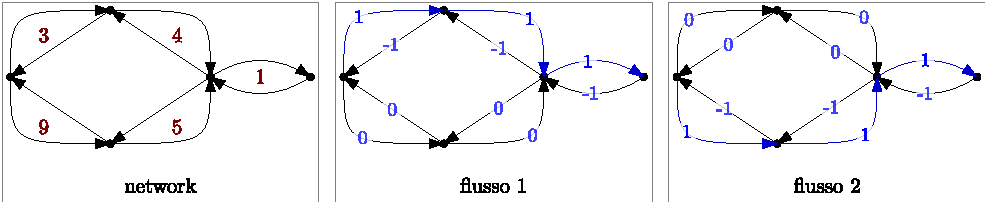
\includegraphics[width=1\textwidth ]{images/flussiCapDistinte.pdf}
\end{center}
è un contro-esempio valido per l'affermazione, quest'ultima risulta quindi falsa.
\begin{esercizio}
\end{esercizio}
Si consideri una network con source $s$ e sink $t$ in cui ogni vertice $v$ ha una \textit{lista di preferenza} sui suoi vertici adiacenti, si assume che quando si esegue una DFS su tale network, i vertici vengono visitati seguendo l'ordine di tale preferenza, ad esempio, se il vertice $v$ ha come lista $(u,x,y)$, allora quando viene visitato per la prima volta, il prossimo vertice che verrà visitato durante la DFS sarà $u$ (se non ancora visitato), altrimenti, $x$, se anche quest'ultimo è stato già visitato, si procederà con $y$. Fornire un'esempio di network in cui l'algoritmo di Ford Fulkerson, utilizzando la DFS con preferenza durante la ricerca del cammino da $s$ a $t$ nel grafo residuo, termina eseguendo un numero esponenziale di passi.
\begin{esercizio}
\end{esercizio}
Sia $P$ un politopo definito come segue 
$$P=\{\x\in\R^n \ : \ A\x\le\bb, \ \x\ge \mathbf 0\} $$
si assume che $P\ne \emptyset$. Dimostrare le seguenti affermazioni\begin{enumerate}
    \item esiste un vettore $\bc$ tale per cui il problema $$\max_{\x\in P}\bc^T\x$$ ha un'unica soluzione ottimale.
    \item assumendo che $|P|\ge 2$, esiste un vettore $\bc$ tale per cui il  problema $$\max_{\x\in P}\bc^T\x$$
    ha infinite soluzioni ottimali.
\end{enumerate}\bigskip 

\noindent \textg{Soluzione}: Il primo punto è banale, dato che si può usare la definizione di vertice, si procede quindi con il secondo.

Si può assumere che $P$ abbia almeno 2 vertici. Siano $\mathbf u,\mathbf v$ due vertici adiacenti, ossia due BFS associate alle basi $\mathcal{B},\mathcal{B}'$ tali per cui $$ |\mathcal{B}\cap \mathcal{B}'|=|\mathcal{B}|-1$$
Essendo $\mathbf u,\mathbf v$ due punti in $\R^n$, esistono infiniti iperpiani passanti per entrambi, si deve considerare un particolare iperpiano $H$ che definisce la faccia di $P$ contenente $\mathbf u,\mathbf v$. Tale iperpiano è definito come i punti $\x$ che soddisfano $$\bc^T\x=\alpha $$
per qualche $\bc\in\R^n,\alpha\in \R$. Tale $\bc$ definisce la funzione obiettivo per cui $\mathbf u,\mathbf v$  sono soluzioni ottimali. Il problema in questo caso ha due soluzioni ottimali, essendo $P$ convesso, ne ha infinite.
\begin{esercizio}
\end{esercizio}
Si consideri il seguente LP \begin{eqnarray*}
    \max \bc^T\x\\ A\x\le\bb \\ \x\ge \mathbf 0 
\end{eqnarray*}
dove la matrice $A$ ha $m$ righe ed $n$ colonne.
Assumendo che il problema non ha soluzioni degenere, dimostrare che se $\x^*$ è una soluzione ammissibile con esattamente $m$ componenti diverse da 0, allora $\x^*$ è una BFS.\bigskip 

\noindent \textg{Soluzione}: $\x^*$ è una BFS se e solo se è un vertice del poliedro delle soluzioni ammissibili. Si pone per assurdo che $\x^*$ non è un vertice, allora è una combinazione convessa dei vertici 
$$ \x^* = \sum_i \beta_i \x^i$$
dove $\x^i$ è l'$i$-esimo vertice. Per definizione di combinazione convessa, i termini $\beta_i$ sono positivi, inoltre i vertici, essendo soluzioni, hanno anche essi ogni componente maggiore o uguale di zero. Ogni vertice per assunzione non è degenere, ha quindi $m$ componenti diverse da zero, essendo che due vertici distinti hanno almeno una componente tale per cui, in un vertice è uguale a zero mentre nell'altro è positiva, si ha che, per ogni $\alpha,\alpha' >0$, il termine 
$$ \alpha\x^i+\alpha'\x^j, \ \ \ i\ne j$$
ha \textit{almeno} $m+1$ componenti diverse da zero. Essendo che $\x^*$ è somma di almeno due vertici pesati da coefficienti positivi, si ha che $\x^*$ ha almeno $m+1$ componenti diverse da zero, ma ciò va in contraddizione con l'assunzione che tali componenti siano esattamente $m$, è quindi impossibile che $\x^*$ non sia un vertice.
\begin{esercizio}
\end{esercizio}
Si risolva il seguente LP con il metodo del simplesso \begin{eqnarray*}
    \max 2x_1+x_2-x_3\\ 
    x_1+2x_2+x_3+x_4=8\\ 
    -x_1+x_2-2x_3+x_5=4\\ 
    x_1,x_2,x_3,x_4,x_5\ge 0
\end{eqnarray*}\bigskip 

\noindent\textg{Soluzione}: La base $\mathcal B=\{4,5\}$ è chiaramente ammissibile, si partirà da questa per applicare il metodo del simplesso
\begin{center}
    \begin{tabular}{|l}
$\mathcal B = \{4,5\}$ \\ \hline
$x_4=-x_1-2x_2-x_3+8$ \\
$x_5=x_1-x_2+2x_3+4$ \\ \hline
$z=2x_1+x_2-x_3$
\end{tabular}
\end{center}
\begin{center}
    \begin{tabular}{|l}
$\mathcal B = \{1,5\}$ \\ \hline
$x_1=-x_4-2x_2-x_3+8$ \\
$x_5=-x_4-3x_2+x_3+12$ \\ \hline
$z=-2x_4-3x_2-3x_3+16$
\end{tabular}
\end{center}
La base $\{1,5\}$ è ottimale, l'ottimo del problema è 16 e la soluzione ottimale è $\begin{bmatrix}
    8&0&0&0&16
\end{bmatrix}^T$. 
\begin{esercizio} 
\end{esercizio}
Siano $(P)$ e $(D)$ una coppia di problemi primario-duale.
$$\begin{matrix}
        \max \  \mathbf c^T\mathbf x\\ 
        A\mathbf x \le \mathbf b \\ 
        \mathbf x \ge 0 
    \end{matrix} \ \ \ \ \ \  \begin{matrix}
        \min \  \mathbf b^T\mathbf y\\ 
        A^T\mathbf y \ge \mathbf c \\ 
        \mathbf y \ge 0 
    \end{matrix}$$
 Se $\x$ è una soluzione per $(P)$, e $\y$ è una soluzione per $(D)$, allora 
$$ \bc^T\x\le \bb^T\y$$
Fornire un'esempio di una coppia di problemi primario-duale, insieme ad una soluzione $\x^*$ per il primario e $\y^*$ per il duale, tali per cui 
$$ \bc^T\x^*< \bb^T\y^*$$\bigskip

\noindent \textg{Soluzione}: Il problema primario è 
\begin{eqnarray*}
    \max x_1\\ x_1+x_2\le 1 \\ x_1,x_2\ge 0
\end{eqnarray*}
il duale è \begin{eqnarray*}
    \min y_1 \\ 
    y_1\ge 1 \\ 
\end{eqnarray*}
le soluzioni sono $$ \x^*=\begin{bmatrix}
    \nicefrac{1}{2}\\ \nicefrac{1}{2}
\end{bmatrix} \ \ \ \ \y^*=\begin{bmatrix}
    1\\1
\end{bmatrix}$$
\begin{center}
    \includegraphics[width=0.6\textwidth ]{images/es8.eps}
\end{center}
la disuguaglianza sulle funzioni obiettivo è stretta 
\begin{eqnarray*}
    \bc^T\x^*<\bb^T\y^*\\
    x_1^*<y_1^*\\ 
    \frac{1}{2}<1
\end{eqnarray*}
\begin{esercizio}
\end{esercizio}
Si consideri il seguente programma lineare parametrizzato da due valori reali $\gamma,\delta$
\begin{eqnarray*}
    \max  \ x_1+\gamma x_2\\ 
    2x_1+x_2\le 5\\ 
    x_1+3x_2\le \delta \\ 
    x_1,x_2\ge 0 
\end{eqnarray*}
per quali valori di $\gamma,\delta$ la soluzione $\x^*=\begin{bmatrix}
    2 & 1
\end{bmatrix}^T$ è ottimale?\bigskip

\noindent
\textg{Soluzione}: è utile un'osservazione, si noti come il secondo vincolo del programma lineare è soddisfatto da $\x^*$ se e solo se $\delta\ge 5$
$$x_1+3x_2 = 2+3 = 5 \le \delta \implies \delta \ge 5 $$
Si noti inoltre che se $\delta > 5$ il secondo vincolo è slack per $\x^*$, questo semplifica la dimostrazione. Il duale del LP è \begin{eqnarray*}
\min 5y_1+\delta y_2\\ 
2y_1+y_2\ge 1\\ 
y_1+3y_2\ge \gamma \\ 
\y>\mathbf 0
\end{eqnarray*} 
Si vuole usare il teorema degli slack complementari per dimostrare che esiste una soluzione $\y^*$ per il duale, il cui ottimo coincide con il valore della funzione obiettivo del primario valutata su $\x^*$. \begin{itemize}
    \item \textbf{caso $\delta>5$)} Si assume che $\x^*$ è ottimale, sia $\y^*$ una soluzione ottimale per il duale, essendo che $x_1^*,x_2^*>0$, i due vincoli per $\y^*$ sono binding, inoltre, $y^*_2=0$ perché il secondo vincolo del primario è slack per $\x^*$.
$$
\begin{matrix}
    2y^*_1= 1\\ 
y^*_1= \gamma \\ 
\end{matrix}\implies \y^*=\begin{bmatrix}
    0.5 & 0
\end{bmatrix}^T
$$
I valori delle funzioni obiettivo coincidono 
\begin{eqnarray*}
    5y^*_1+\delta y^*_2=x^*_1+\gamma x^*_2\\ 
    5\gamma=2+\gamma \\ 
    5\frac{1}{2}=2+\frac{1}{2}
\end{eqnarray*}
$\x^*$ è una soluzione ottimale. 
\item \textbf{caso $\delta=5$)} in questo caso non si può annullare $y^*_2$, risolvendo il sistema si ottiene il valore di $\y^*$ in funzione di $\gamma$
$$\begin{matrix}
    2y^*_1+y^*_2= 1\\ 
y^*_1+3y^*_2= \gamma \\ 
\end{matrix} \implies 
\begin{matrix}
    y_1^*=\gamma-\frac{1}{2}\\ 
    y_2^*=-2\gamma+\frac{3}{2}
\end{matrix}
$$
$\x^*$ è ottimale se le funzioni obiettivo coincidono, essendo $\delta = 5$, si deve risolvere 
$$ 5y^*_1+\delta y^*_2=x^*_1+\gamma x^*_2$$
per $\gamma$\begin{eqnarray*}
    5(\gamma-\frac{1}{2})+5 (-2\gamma+\frac{3}{2})=2+\gamma \implies 
\\ \gamma = \frac{1}{2}
\end{eqnarray*}
\end{itemize}
In definitiva, il punto $\x^*=\begin{bmatrix}
    2 & 1
\end{bmatrix}^T$ è una soluzione ottimale se $\gamma = \frac{1}{2}$ e $\delta\ge 5$.







\begin{esercizio}
\end{esercizio}
Si consideri un LP in $n$ variabili ed $m$ vincoli di cui $P$ è il poliedro delle soluzioni e $P_I$ è l'inviluppo convesso di $P\cap \Z^n$. Sia $\mathcal B$ una base ammissibile, e sia $i$ un indice fissato in $\mathcal B$. Sia $N$ l'insieme degli indici che non sono contenuti nella base 
$$N=\{1,2,\dots n\}\backslash\mathcal B $$
 Se $\x$ è la BFS associata a tale base, la seguente è soddisfatta 
$$ x_i=p_i+\sum_{j\in N}Q_{i,j}x_j$$
Si ricordi che la matrice $Q$ ed il vettore $\mathbf p$ sono univocamente definiti come nel lemma \ref{lemma_tableau}. Dimostrare che per ogni soluzione $\x^*$ in $P_I$, la seguente 
$$\sum_{j\in N}(Q_{i,j}-\lfloor Q_{i,j}\rfloor)x^*_j\ge p_i-\lfloor p_i\rfloor $$
è soddisfatta.
\end{document}